\documentclass[12pt,letterpaper]{article}
\usepackage[margin=1in]{geometry}
\usepackage[utf8]{inputenc}
\usepackage{longtable}
\usepackage{graphicx}
\usepackage{caption}
\usepackage{subcaption}
\usepackage{svg}
\usepackage{amsmath}
\usepackage{float}
\usepackage{array}
\usepackage{xr}
\usepackage[nottoc,numbib]{tocbibind}
\usepackage{csvsimple}
\usepackage{algpseudocode}
\usepackage{hyperref}
\usepackage{soul}
\usepackage{multicol}
\usepackage{acronym}  % Add this line
\usepackage[acronym,toc]{glossaries}  % Add this line
\usepackage{multirow}
\setcounter{secnumdepth}{4}
\maxdeadcycles=1000
\renewcommand{\topfraction}{.85}
\renewcommand{\textfraction}{.1}
\renewcommand{\floatpagefraction}{.85}
% Create glossaries
\makeglossaries

% Glossary entries

\newglossaryentry{wetland}{
  name=wetland,
  description={land consisting of marshes or swamps; saturated land}
}

\newglossaryentry{marsh}{
  name=marsh,
  description={a wetland that is dominated by herbaceous rather than woody plant species}
}

\newglossaryentry{bog}{
  name=bog,
  description={a wetland that accumulates peat, a deposit of dead plant material—often mosses, and in a majority of cases, sphagnum moss}
}

\newglossaryentry{fen}{
  name=fen,
  description={a type of peat-accumulating wetland that receives some drainage from surrounding mineral soils and usually supports marsh-like vegetation}
}

\newglossaryentry{swamp}{
  name=swamp,
  description={a wetland that is forested, often with standing or slow-moving water}
}





% Remove paragraphs automatic indentation
\setlength{\parindent}{0pt}

% Add an empty line after a paragraph
\usepackage{parskip}

\title{\textbf{UMoncton CCNB-Innov Project} 
\textit{Technical Report}}
\author{M-A. Blais, M. Akhloufi \\
Perception, Robotics and Intelligent Machines (PRIME), \\
Université de Moncton, \\
18 Antonine Maillet Ave. \\
Moncton, NB E1A 3E9}
\date{TBD 2024}

\externaldocument{./class_all_section/class_accuracies}
\externaldocument{./class_all_section/class_ensemble_figures}
\externaldocument{./class_all_section/class_reduction_figures}
\externaldocument{./class_all_section/class_reduction_ensemble_figures}
\externaldocument{./class_all_section/class_features_acc}


\externaldocument{./reg_section_all/dimred_results}
\externaldocument{./general/features}
\externaldocument{./general/res_analysis}


\externaldocument{./reg_section_all/reg_mse}
\externaldocument{./reg_section_all/reg_training_figures}
\externaldocument{./reg_section_all/reg_ensemble}
\externaldocument{./reg_section_all/reg_featred_mse}
\externaldocument{./reg_section_all/class_grouping}

\externaldocument{./reg_section_all/reg_featred_graphs}
\externaldocument{./reg_section_all/reg_featred_ensemble_graphs}
\externaldocument{./reg_section_all/reg_featred_ensemble_tables}

\externaldocument{./reg_section_all/regression_models}
\externaldocument{./reg_section_specific/training_mse}
\externaldocument{./reg_section_specific/reg_training_figures}
\externaldocument{./reg_section_specific/reg_featred_mse}
\externaldocument{./reg_section_specific/reg_featred_ensemble_graphs}
\externaldocument{./reg_section_specific/reg_featred_ensemble_tables}
\externaldocument{./reg_section_specific/class_grouping}

\externaldocument{./reg_section_xtra/training_mse}


\externaldocument{./reg_section_specxtra/training_mse}
\externaldocument{./reg_section_specxtra/reg_training_figures}
\externaldocument{./reg_section_specxtra/reg_featred_mse}
\externaldocument{./reg_section_specxtra/reg_featred_ensemble_graphs}
\externaldocument{./reg_section_specxtra/reg_featred_ensemble_tables}
\externaldocument{./reg_section_specxtra/class_grouping}



\externaldocument{./causalml_section/tables}
\externaldocument{./causalml_section/graphs}

\externaldocument{./class_specific_section/training_accuracy}
\externaldocument{./class_specific_section/class_ensemble_figures}
\externaldocument{./class_xtra_section/class_feature_acc}

\externaldocument{./class_specificxtra_section/class_ensemble_figures}
\externaldocument{./class_specificxtra_section/class_feature_acc}


\externaldocument{./analysis/res1}
\externaldocument{./analysis/res2}

\externaldocument{./analysis/res1_reg}
\externaldocument{./analysis/res2_reg}



\begin{document}

\maketitle
\thispagestyle{empty}



\clearpage 
\thispagestyle{plain}
\tableofcontents % This will create the Table of Contents

\section*{Abstract}

\clearpage
\printglossaries

\clearpage
\section*{List of Acronyms}
\begin{acronym}
\acro{ML}[ML]{Machine Learning}
\acro{WESP-AC}[WESP-AC]{Wetland Ecosystem Services Protocol for Atlantic Canada}
\acro{PCA}[PCA]{Principal Component Analysis}
\acro{CNN}[CNN]{Convolutional Neural Network}
\acro{CI}[CI]{Causal Inference}
\acro{EF}[EF]{\ac{EF}}
\acro{NB}[NB]{New-Brunswick}
\acro{NRNB}[NRNB]{Natural ressources NB}
\acro{WS}[WS]{Water Storage \& Delay}
\acro{PR}[PR]{Phosphorus Retention}
\acro{SR}[SR]{Sediment Retention \& Stabilization}
\acro{NR}[NR]{Nitratre Remove \& Retention}
\acro{SFST}[SFST]{Stream Flow Support}
\acro{VT}[VT]{Variance Threshold}


% Add more acronyms here
\end{acronym}



\section{Introduction}
This document should be served as supplementary file for the report.
It contains various results not included in the main document.


\section{Classification}\label{sec:class}
First, in section \ref{sec:class_all}, we train our algorithms using our D1 dataset.
Section \ref{sec:class_spec}, \ref{sec:class_xtra} and \ref{sec:class_allxtra} use the respective D2, D3 and D4 datasets.


\subsection{All Features (D1)}\label{sec:class_all}
This section trains our algorithms using all features provided by the WESP-AC 3.4, with the exception of the unnecessary features.
We compare our results using multiple data filling methods, however we only present the best performing methods.
First, we present the training results and the ensemble learning approach using all features in section \ref{sec:class_all_results}.
Our ensemble learning algorithm consists of combining the top five best performing algorithms and average out the predictions.
Section \ref{sec:class_all_featred} presents a feature reduction approach using the results from section \ref{sec:class_all_results}.

\subsubsection{Training Results}\label{sec:class_all_results}
Table \ref{tab_class_all:model_accuracies_best} provides an overview of some of the best performing algorithms with specific filling methods.


\begin{table}[H]
\centering
\begin{tabular}{|c|c|c|c|}
\hline
\textbf{Function} & \textbf{Model} & \textbf{Data} & \textbf{Accuracy} \\
\hline
\multirow{2}{*}{PR} & GradientBoosting & BFill, FFill, Interpolated, Mean, Mode & 95.0\% \\
 & RandomForest & BFill, FFill, Interpolated, Mean, Median & 95.0\% \\
\hline
NR    & LogisticReg. & BFill, Custom, FFill, Interpolated, KNN, Mean & 81.0\% \\
\hline
SR    & GradientBoosting & Iterative, Median, Mode & 90.0\% \\
\hline
WS    & GradientBoosting & BFill, Interpolated, Mode, KNN, Mean, Median & 95.0\% \\
\hline
SFST  & DecisionTree & Iterative, Mode & 100.0\% \\
\hline
\multirow{2}{*}{PR Ben.} & LinearDiscriminant & BFill, Custom, Iterative & 95.0\% \\
 & GradientBoosting & BFill, FFill, Interpolated, Mean, Mode & 95.0\% \\
\hline
NR Ben. & GradientBoosting & BFill, Custom, FFill & 95.0\% \\
\hline
SR Ben.& Ridge& All Data & 100.0\% \\
\hline
WS Ben. & GradientBoosting & BFill, Interpolated, Mode & 95.0\% \\
\hline
\multirow{2}{*}{SFST Ben.} & DecisionTree & Mode & 95.0\% \\
 & GradientBoosting & BFill & 81.0\% \\
\hline
\end{tabular}
\caption{Best Model Accuracies}
\label{tab_class_all:model_accuracies_best}
\end{table}

In this table, each \ac{EF} is shown with the accuracy of the best performing model and data filling method.


To increase the validity of using \ac{ML} for this task, we propose ensemble learning.
The results from ensemble learning are shown in section \ref{sec:class_ensemble}.
We also propose feature selection which consists of using a limited amount of features to achieved similar.
Feature selection would enable us to use less features (E.g 10) to achieve similar results.
Feature selection is presented in section \ref{sec:class_all_featred}.


\paragraph{Ensemble Learning}\label{sec:class_all_ensemble}
To increase the performance of our algorithms, we propose using ensemble learning to combine multiple models.
Overall, the ensemble learning did not increase the performance of our algorithms, as shown in table \ref{tab_class_all:class_ensemble}.
\begin{table}[H]
\centering
\begin{tabular}{|c|c|c|}
\hline
\textbf{Function} & \textbf{Accuracy} & \textbf{Ensemble Accuracy} \\
\hline
PR      & 95.24\% & 95.24\% \\
\hline
NR      & 80.59\% & 80.59\%\\
\hline
SR      & 90.48\% & 85.71\%\\
\hline
WS      & 95.24\% & 95.24\%\\
\hline
SFST    & 100.0\% & 95.24\%\\
\hline
PR Ben. & 95.24\% & 90.48\%\\
\hline
NR Ben. & 95.24\% & 95.24\%\\
\hline
SR Ben. & 100.0\% & 100.0\%\\
\hline
WS Ben. & 95.24\% & 95.24\%\\
\hline
SFST Ben. & 95.24\% & 95.24\%\\
\hline
\end{tabular}
\caption{Ensemble Model Accuracies}
\label{tab_class_all:class_ensemble}
\end{table}

Figures \ref{fig:ensemble_pr}, \ref{fig:ensemble_nr}, \ref{fig:ensemble_sr}, \ref{fig:ensemble_ws}, \ref{fig:ensemble_sfst}, \ref{fig:ensemble_pr_benefit}, \ref{fig:ensemble_nr_benefit}, \ref{fig:ensemble_sr_benefit}, \ref{fig:ensemble_ws_benefit} and \ref{fig:ensemble_sfst_benefit} show the confusion matrices for each EFs using ensemble learning.



\subsubsection{Feature Selection}\label{sec:class_all_featred}
Feature selection consists of using techniques to reduce the number of features required to train the algorithms while achieving similar results.
In this section we explore the three feature reduction techniques, presented in section \ref{sec:PA}.

Using the accuracy as metric, we compare the algorithms for each ecosystem function trained with reduced features.
The best performing algorithm for each function was selected based on accuracy from table \ref{tab_class_all:class_ensemble}.
Each algorithm was trained with the three reduction techniques with features ranging from all features to only tow features.
Figures \ref{fig:nr_class} to \ref{fig:sfst_ben_class} show the results for each \ac{EF} with the three reduction techniques.

Interesting behavior can be observed when analyzing the results from these figures.
Tables \ref{tab_class_all:ensemble_class_acc} and \ref{tab_class_all:ensemble_prop_class_acc} respectively show the best overall accuracies and the best using two features.
The overall accuracy consists of the method that achieved the best accuracy regardless of the number of features.
The best two features takes the best accuracy from the three method which only used two feature to predict the class.





\paragraph{Ensemble Learning}
To increase the performance of our feature reduction approach, we propose using ensemble learning.
This is proposed to average out errors to increase the performance without retraining or the need for complex algorithms.
Our ensemble model, for each \ac{EF}, is based on the top five models achieved from the feature reduction with no more than 10 features per model.
Table \ref{tab_class_all:ensemble_reduction_class} show the performance for each function before and after the ensemble learning.

% Table for proportionate accuracy
\begin{longtable}{|p{2cm}|p{2cm}|p{2cm}|p{2cm}|p{6cm}|}
\hline
\textbf{Function} & \textbf{Best Acc.} & \textbf{2nd Best Acc.} & \textbf{Ensemble Learning Acc.} & \textbf{Features Used} \\ \hline
PR & 95.24\% & 95.24\% & 95.24\% & F1, F14, F21, F23, F24, F28, F29, F30, F41, F43, F44, F45, F46 \\ \hline
NR & 76.19\% & 76.19\% & 76.19\% & F43, F44, F45, F46 \\ \hline
SR & 90.48\% & 80.95\% & 85.71\% & F1, F14, F24, F25, F28, F29, F30, F31, F3e, F43, F44, F45, F46, OF22 \\ \hline
WS & 90.48\% & 90.48\% & 90.48\% & F1, F29, F31, F43, F44, F45, F46, F65 \\ \hline
SFST & 95.24\% & 95.24\% & 95.24\% & F43, F44, F45, F46 \\ \hline
PR Benefit & 85.71\% & 85.71\% & 85.71\% & F14, F41, F43, F44, F46, F47, F55 \\ \hline
NR Benefit & 90.48\% & 90.48\% & 90.48\% & F1, F14, F31, F3d, F41, F43, F46, OF10, OF19, OF9 \\ \hline
SR Benefit & 100.00\% & 100.00\% & 100.00\% & F1, F14, F23, F25, F28, F29, F3e, F41, F43, F44, F45, F46, OF19, OF21 \\ \hline
WS Benefit & 95.24\% & 95.24\% & 95.24\% & F3c, F3e, F49, F50, F51, F52, F54, OF17, OF23, OF38, OF5, OF7, OF9 \\ \hline
SFST Benefit & 90.48\% & 85.71\% & 90.48\% & F1, F14, F23, F30, F3e, F43, F44, F45, F46 \\ \hline
\caption{Ensemble Learning Accuracy}
\label{tab_class_all:ensemble_reduction_class}
\end{longtable}
In this table, the first column represents the \ac{EF}, while the second and third represent the best and second best accuracy from section \ref{sec:class_all_featred} with a maximum of 10 features.
The fourth column represent the accuracy of the ensemble learning model while the last column consists of the features of all five models used for ensemble learning.


\subsection{Specific Features (D2)}\label{sec:class_spec}
In this section we train the same algorithms as the previous section.
However, the algorithms are trained only and their respective specific features using the D2 dataset.
Our goal for this section is to reduce possible noise that can be caused by using all features.
Similarly to the previous section, we compare using all features versus using feature reduction techniques and ensemble learning.


\subsubsection{Training Results}
In terms of training results, we present an overview of the best performing algorithms and filling method.
Our training results are more exploratory and are used to pinpoint specific algorithms and data filling methods for each \ac{EF}.
Table \ref{tab_class:spec_model_accuracies_best} provides an overview of some of the best performing algorithms and data.


\begin{table}[H]
\centering
\begin{tabular}{|c|c|c|c|}
\hline
\textbf{Function} & \textbf{Model} & \textbf{Data} & \textbf{Accuracy} \\
\hline

PR & RidgeClassifier & All Data & 95.2\% \\
\hline
NR & RidgeClassifier & All Data & 85.7\% \\
\hline
SR & SGDClassifier & BFill, Mean & 95.2\% \\
\hline
WS & GradientBoostingClassifier & All Data & 100.0\% \\
\hline
SFST & DecisionTreeClassifier & All Data & 95.2\% \\
\hline
PR Ben. & DecisionTreeClassifier & BFill & 100.0\% \\
\hline
NR Ben. & SVC & All Data & 100.0\% \\
\hline
SR Ben. & RidgeClassifier & All Data & 100.0\% \\
\hline
WS Ben. & RandomForestClassifier & Custom, FFill, Interpolated, Iterative & 95.24\% \\
\hline
SFST Ben. & MLPClassifier & Interpolated & 71.43\% \\
\hline

\end{tabular}
\caption{Best Model Accuracies}
\label{tab_class:spec_model_accuracies_best}
\end{table}

In this table, we present which model and data filling method achieved the best accuracy for each \ac{EF}.



\subsubsection{Ensemble Learning}
We also combine the best performing algorithms using ensemble learning.
Overall, the ensemble learning did not increase the performance of our algorithms, as shown in table \ref{tab_spec:class_ensemble}.
\begin{table}[H]
\centering
\begin{tabular}{|c|c|c|}
\hline
\textbf{Function} & \textbf{Accuracy} & \textbf{Ensemble Accuracy} \\
\hline
PR      & 95.24\% & 95.24\% \\
\hline
NR      & 85.71\% & 85.71\%\\
\hline
SR      & 95.24\% & 95.24\%\\
\hline
WS      & 100.0\% & 100.0\%\\
\hline
SFST    & 95.24\% & 95.24\%\\
\hline
PR Ben. & 100.0\% & 100.0\%\\
\hline
NR Ben. & 100.0\% & 100.0\%\\
\hline
SR Ben. & 100.0\% & 100.0\%\\
\hline
WS Ben. & 95.24\% & 95.24\%\\
\hline
SFST Ben. & 71.43\% & 71.43\%\\
\hline
\end{tabular}
\caption{Ensemble Model Accuracies}
\label{tab_spec:class_ensemble}
\end{table}

Figures \ref{fig_class:spec_ensemble_pr}, \ref{fig_class:spec_ensemble_nr}, \ref{fig_class:spec_ensemble_sr}, \ref{fig_class:spec_ensemble_ws}, \ref{fig_class:spec_ensemble_sfst}, \ref{fig_class:spec_ensemble_pr_benefit}, \ref{fig_class:spec_ensemble_nr_benefit}, \ref{fig_class:spec_ensemble_sr_benefit}, \ref{fig_class:spec_ensemble_ws_benefit} and \ref{fig_class:spec_ensemble_sfst_benefit} show the confusion matrices for each EFs using ensemble learning.

\subsubsection{Feature Selection}
We also use the three feature reduction techniques to reduce the features used while trying to achieve similar results.
We compare both the overall accuracy and the best accuracy using only two features.
Tables \ref{tab_class_spec:ensemble_class_acc} and \ref{tab_class_spec:ensemble_prop_class_acc} respectively show the best overall accuracies and the best using two features.

\paragraph{Ensemble Learning}
Table \ref{tab_class_spec:ensemble_reduction} show the performance for each \ac{EF} before and after ensemble learning.

% Table for proportionate accuracy
\begin{longtable}{|p{2cm}|p{2cm}|p{2cm}|p{2cm}|p{6cm}|}
\hline
\textbf{Function} & \textbf{Best Acc.} & \textbf{2nd Best Acc.} & \textbf{Ensemble Learning Acc.} & \textbf{Features Used} \\ \hline
PR & 90.48\% & 90.48\% & 90.48\% & F17, F20, F21, F23, F24, F28, F29, F31, F33, F34, F35, F36, F43, F44, F45, F49, OF22, OF26, OF27 \\ \hline
NR & 76.19\% & 76.19\% & 76.19\% & F1, F24, F28, F31, F3c, F43, F44, F45 \\ \hline
SR & 80.95\% & 80.95\% & 80.95\% & F17, F28, F29, F31, F33, F34, F35, F36, F43, F44, F45, F49, F9, OF22 \\ \hline
WS & 100.00\% & 100.00\% & 95.24\% & F20, F28, F31, F3c, F3d, F3e, F43, F44, F45, F49, OF22, OF26 \\ \hline
SFST & 95.24\% & 95.24\% & 95.24\% & F1, F14, F24, F31, F43 \\ \hline
PR Benefit & 95.24\% & 95.24\% & 90.48\% & F41, F48, F50, F52, OF19, OF20, OF21, OF22, OF23, OF24 \\ \hline
NR Benefit & 90.48\% & 90.48\% & 85.71\% & F13, F41, F50, F51, F52, OF10, OF19, OF20, OF21, OF22, OF24, OF9 \\ \hline
SR Benefit & 100.00\% & 100.00\% & 100.00\% & F24, F28, F41, OF19, OF20, OF21, OF24 \\ \hline
WS Benefit & 95.24\% & 95.24\% & 95.24\% & F51, OF17, OF18, OF23, OF24, OF8 \\ \hline
SFST Benefit & 57.14\% & 57.14\% & 57.14\% & F50, OF18, OF22, OF25, OF28 \\ \hline
\caption{Ensemble Learning Accuracy}
\label{tab_class_spec:ensemble_reduction}
\end{longtable}


\subsection{Extra(D3)}\label{sec:class_xtra}
This section is used to train our various classification algorithms on D3, which consists of extra features collected outside the WESP-AC.

\subsubsection{Training Results}
In this section, we present an overview of the best performing algorithms and filling method.
Table \ref{tab_class:xtra_model_accuracies_best} provides an overview of some of the best performing algorithms and data.


\begin{table}[H]
\centering
\begin{tabular}{|c|c|c|c|}
\hline
\textbf{Function} & \textbf{Model} & \textbf{Data} & \textbf{Accuracy} \\
\hline

PR & SVC & Iterative & 95.24\% \\
\hline
NR & SVC & FFil & 71.43\% \\
\hline
SR & DecisionTreeClassifier & Mean & 61.90\% \\
\hline
WS & GradientBoostingClassifier & FFill & 71.43\% \\
\hline
SFST & DecisionTreeClassifier & Mode, KNN & 71.43\% \\
\hline
PR Ben. & SGDClassifier & Interpolated & 85.71\% \\
\hline
NR Ben. & KNeighborsClassifier & KNN & 66.67\% \\
\hline
SR Ben. & SVC & Mean & 76.19\% \\
\hline
WS Ben. & DecisionTreeClassifier & Custom, BFill & 71.43\% \\
\hline
SFST Ben. & MLPClassifier, GaussinNB & FFil & 71.43\% \\
\hline

\end{tabular}
\caption{Best Model Accuracies}
\label{tab_class:xtra_model_accuracies_best}
\end{table}




\subsubsection{Ensemble Learning}
We also use the best performing five algorithms with their respective filling method and combined them.
Overall, the ensemble learning did not increase the performance of our algorithms, as shown in table \ref{tab_xtra:class_ensemble}.
\begin{table}[H]
\centering
\begin{tabular}{|c|c|c|}
\hline
\textbf{Function} & \textbf{Accuracy} & \textbf{Ensemble Accuracy} \\
\hline
PR      & 95.23\% & 90.48\% \\
\hline
NR      & 71.42\% & 61.90\%\\
\hline
SR      & 61.90\% & 61.90\%\\
\hline
WS      & 71.42\% & 66.66\%\\
\hline
SFST    & 71.42\% & 66.66\%\\
\hline
PR Ben. & 85.71\% & 76.19\%\\
\hline
NR Ben. & 66.66\% & 66.66\%\\
\hline
SR Ben. & 76.19\% & 76.19\%\\
\hline
WS Ben. & 71.42\% & 66.66\%\\
\hline
SFST Ben. & 71.42\% & 66.66\%\\
\hline
\end{tabular}
\caption{Ensemble Model Accuracies}
\label{tab_xtra:class_ensemble}
\end{table}

\subsubsection{Feature Selection}
Similar to previous section, we perform feature reduction using our three techniques on this data.
We present both the best overall accuracies using any number of features and the best accuracy fr each \ac{EF} using only two features.
Tables \ref{tab_class_xtra:ensemble_class_acc} and \ref{tab_class_xtra:ensemble_prop_class_acc} respectively show the best overall accuracies and the best using two features.


\paragraph{Ensemble Learning}
Using a maximum of 10 features per model, we combine the top five for ensemble learning to increase the performance.
Table \ref{tab_class_xtra:ensemble_reduction}, in the annexe, show the performance for each function before and after ensemble learning.



\subsection{Specific Features and Extra (D5)}\label{sec:class_allxtra}
In this section, we train our algorithms and compare them using our D4 dataset which consists of the specific and extra \textbf{features}.
\subsubsection{Training Results}
In terms of training results ,table \ref{tab_class:specxtra_model_accuracies_best} provides the overview of some of the best performing models.


\begin{table}[H]
\centering
\begin{tabular}{|c|c|c|c|}
\hline
\textbf{Function} & \textbf{Model} & \textbf{Data} & \textbf{Accuracy} \\
\hline

PR & RidgeClassifier & All Data & 95.4\% \\
\hline
NR & MLPClassifier & Interpolated, Itterative & 85.71\% \\
\hline
SR & SVCClassifier & BFill, Mean & 90.48\% \\
\hline
WS & GradientBoostingClassifier & BFill & 100.0\% \\
\hline
SFST & GradientBoostingClassifier & All Data & 95.24\% \\
\hline
PR Ben. & RidgeClassifier
 & All Data & 100.0\% \\
\hline
NR Ben. & AdaBoostClassifier & All Data & 95.24\% \\
\hline
SR Ben. & RidgeClassifier, 
 & All Data & 100.0\% \\ 
 \hline
WS Ben. & AdaBoostClassifier & Median, Mean, Interpolated, Iterative & 95.24\% \\
\hline
SFST Ben. & DecisionTreeClassifier & Median & 80.95\% \\
\hline

\end{tabular}
\caption{Best Model Accuracies}
\label{tab_class:specxtra_model_accuracies_best}
\end{table}

In this table, each \ac{EF} is shown with their best accuracy achieved with a specific model and data filling methods.



\subsubsection{Ensemble Learning}
The ensemble learning approach using the top five algorithms is shown in table \ref{tab_specxtra:class_ensemble}.
\begin{table}[H]
\centering
\begin{tabular}{|c|c|c|}
\hline
\textbf{Function} & \textbf{Accuracy} & \textbf{Ensemble Accuracy} \\
\hline
PR      & 95.24\% & 95.24\% \\
\hline
NR      & 85.71\% & 80.95\%\\
\hline
SR      & 90.47\% & 95.24\%\\
\hline
WS      & 100.0\% & 95.24\%\\
\hline
SFST    & 95.24\% & 95.24\%\\
\hline
PR Ben. & 100.0\% & 95.24\%\\
\hline
NR Ben. & 95.24\% & 95.24\%\\
\hline
SR Ben. & 100.0\% & 100.0\%\\
\hline
WS Ben. & 95.24\% & 95.24\%\\
\hline
SFST Ben. & 80.95\% & 76.19\%\\
\hline
\end{tabular}
\caption{Ensemble Model Accuracies}
\label{tab_specxtra:class_ensemble}
\end{table}
In this table, each \ac{EF} is shown with the best training accuracy and the ensemble learning results.

Figures \ref{fig_class:specxtra_ensemble_pr}, \ref{fig_class:specxtra_ensemble_nr}, \ref{fig_class:specxtra_ensemble_sr}, \ref{fig_class:specxtra_ensemble_ws}, \ref{fig_class:specxtra_ensemble_sfst}, \ref{fig_class:specxtra_ensemble_pr_benefit}, \ref{fig_class:specxtra_ensemble_nr_benefit}, \ref{fig_class:specxtra_ensemble_sr_benefit}, \ref{fig_class:specxtra_ensemble_ws_benefit} and \ref{fig_class:specxtra_ensemble_sfst_benefit} show the confusion matrices for each \ac{EF} using ensemble learning.

\subsubsection{Feature Selection}
We also perform our three feature reduction techniques on this dataset.
Tables \ref{tab_class_specxtra:ensemble_class_acc} and \ref{tab_class_specxtra:ensemble_prop_class_acc} respectively show the best overall accuracies and the best using two features.


\paragraph{Ensemble Learning}
Table \ref{tab_class_specxtra:ensemble_reduction} show the performance for each function before and after the ensemble learning and the features used.

% Table for proportionate accuracy
% Table for proportionate accuracy
\begin{longtable}{|p{2cm}|p{2cm}|p{2cm}|p{2cm}|p{6cm}|}
\hline
\textbf{Function} & \textbf{Best Acc.} & \textbf{2nd Best Acc.} & \textbf{Ensemble Learning Acc.} & \textbf{Features Used} \\ \hline
PR & 90.48\% & 85.71\% & 85.71\% & F28, F29, F31, F43, F44, F45 \\ \hline
NR & 80.95\% & 76.19\% & 76.19\% & F24, F43, F44, F45 \\ \hline
SR & 80.95\% & 80.95\% & 85.71\% & F28, F31, F34, F35, F43, F44, F45, Federal Class, OF22, Provincial Class \\ \hline
WS & 95.24\% & 90.48\% & 90.48\% & F28, F31, F3e, F43, F44, F45, Federal Class, Hydrogeomorphic, Moss Cover, OF22, Provincial Class, Regime \\ \hline
SFST & 95.24\% & 95.24\% & 95.24\% & F1, F14, F24, F31, F43, Federal Class \\ \hline
PR Benefit & 90.48\% & 90.48\% & 90.48\% & F41, F48, F50, Hydrogeomorphic Class, Living Moss Depth, Moss Cover, OF20, OF21, OF22, OF24, Phragmites, Provincial Class, Regime \\ \hline
NR Benefit & 80.95\% & 80.95\% & 80.95\% & F41, Federal Class, Living Moss Depth, Moss Cover, OF10, OF19, OF21, OF9, Organic Depth, Provincial Class \\ \hline
SR Benefit & 100.00\% & 100.00\% & 100.00\% & F24, F28, F41, Hydrogeomorphic, Moss Cover, OF19, OF20, OF21, Provincial Class, Regime, Surface Water Present \\ \hline
WS Benefit & 95.24\% & 95.24\% & 95.24\% & F51, Living Moss Depth, OF17, OF18, OF23, OF24, OF8, Organic Depth, Soil Type, Vegetation Cover, Woody Canopy Cover \\ \hline
SFST Benefit & 66.67\% & 61.90\% & 71.43\% & Federal Class, Hydrogeomorphic, Living Moss Depth, Moss Cover, OF18, OF22, OF25, OF28, Provincial Class, Regime, Soil Type, Surface Water \\ \hline
\caption{Ensemble Learning Accuracy}
\label{tab_class_specxtra:ensemble_reduction}
\end{longtable}


\newpage


\section{Regression}\label{sec:regression}
Regression is a common type of algorithm often used in \ac{ML} with a key difference to classification.
Classification predicts a class, such as 0 or 1, while regression predicts a continuous value.
In our case, the continuous value would be the score for the function or benefit of an \ac{EF}.
The classification results from \ref{sec:class} have shown great promise and is interesting for the project.
However, the algorithms trained for classification used the normalized scores both for the function and benefit.
In turn, the algorithms are specific to regions, such as for NB, and depend on the calibration wetlands.
If different calibration wetlands are used or the region modified, the algorithms could underperform significantly.
For this reason, we propose using regression to predict the non-normalized scores of the various \ac{EF}.
We use the non-normalize score such that it does our approach does not depend on calibration sites or region.
The data was collected, modified and generated using simple pre-processing techniques as seen from section \ref{sec:data}.
We present our results using all features, specific features, extra features and a combination of both.
We use the Mean Squared Error (MSE) which averages the squares of the errors and is defined in equation \ref{eq:mse}.
\begin{equation}
\text{MSE} = \frac{1}{n} \sum_{i=1}^n (y_i - \hat{y}_i)^2
\label{eq:mse}
\end{equation}

\subsection{All Features(D1)}
Similar to our classification code, we perform a grid search of various regression algorithms.
We trained our algorithms and techniques for the\ac{NR},\ac{PR},\ac{SR},\ac{WS} and \ac{SFST} for both the function and the benefit.
More information about the training procedure can be found within the github under the regression folder.
The algorithms used for regression are explained in table \ref{tab:all_algorithms}.
Similar to classification, we propose comparing the regression algorithms using all features for the \ac{EF}.
We first train our algorithms using all features, implement dimension reduction, features selection and ensemble learning.
\clearpage
\subsubsection{Training Results}
Table \ref{tab:model_reg_all_best} presents the training results using the best algorithm and filling method for each EF.
\begin{table}
\centering
\begin{tabular}{|c|c|c|c|}
\hline
\textbf{Function} & \textbf{Model} & \textbf{Data} & \textbf{RMSE} \\
\hline
PR    & AdaBoostRegressor & mean & 0.12 \\
\hline
NR    & AdaBoostRegressor  & median & 0.15 \\
\hline
SR    & AdaBoostRegressor & median & 0.34 \\
\hline
WS    & AdaBoostRegressor & bfill & 0.25\\
\hline
SFST  & AdaBoostRegressor & ffill & 0.21 \\
\hline
PR Benefit & MLPRegressor &  mean & 1.30 \\
\hline
NR Benefit  & MLPRegressor & iterative & 0.38 \\
\hline
SR Benefit &  RANSACRegressor &  ffill & 0.91 \\
\hline
WS Benefit & AdaBoostRegressor & BFill & 1.25 \\
\hline
SFST Benefit & AdaBoostRegressor & Iterative & 0.49 \\
\hline
\end{tabular}
\caption{Model MSE}
\label{tab:model_reg_all_best}
\end{table}
Figures \ref{fig:pr_reg_training} to \ref{fig:sfst_ben_reg_training} show the best algorithm using various fill methods.


\paragraph{Ensemble Learning}
Ensemble learning consists of combining multiple models to increase the results by averaging out the predictions.
Figures \ref{fig:pr_ensemble} to \ref{fig:sfst_ben_ensemble} show the graphical results of the ensemble learning approach while table \ref{tab:ensmeble} show the MSE.


\begin{longtable}{|p{3cm}|p{4cm}|p{4cm}|}
\hline
\textbf{Function} & \textbf{best} & \textbf{Ensemble}  \\ \hline


PR & 0.12 & 0.4621 \\ \hline
NR & 0.15 & 0.4978\\\hline
SR & 0.34 & 0.4796  \\ \hline
WS & 0.25 & 0.4280  \\ \hline
SFST & 0.21 & 0.5130  \\ \hline

PR Benefit & 1.30 & 1.2220 \\ \hline
NR Benefit & 0.38 & 0.8190 \\ \hline
SR Benefit & 0.91 & 0.9797  \\ \hline
WS Benefit & 0.98 & 0.9945  \\ \hline
SFST Benefit & 0.57 & 0.6444  \\ \hline
\caption{Ensemble Learning Results}
\label{tab:ensmeble}
\end{longtable}
In this table, each \ac{EF} has the overall best accuracy and the ensemble learning which combines the top five models.


\paragraph{Class Grouping}
Similar to classification, our goal for this section is to predict the ratings for a specific site.
We use the regression predictions to classify if a site is lower, moderate or higher.
We first normalized the prediction results using the NB minimum and maximum of each function which are presented in table \ref{tab:norm}.
We also collected the boundaries for each \ac{EF} in NB, which are presented in table \ref{tab:boundaries}

\begin{longtable}{|p{3cm}|p{4cm}|p{4cm}|}
\hline
\textbf{Function} & \textbf{Minimum} & \textbf{Maximum}  \\ \hline

WS & 1.58 & 8.61 \\ \hline
PR & 2.07 & 10.0\\ \hline
NR & 4.10 & 10.0 \\\hline
SR & 2.29 & 10.0 \\ \hline
SFST & 0.0 & 7.71 \\ \hline

WS Benefit & 0.08 & 10.0 \\ \hline
PR Benefit & 0.49 & 10.0\\ \hline
NR Benefit & 0.71 & 10.0 \\ \hline
SR Benefit & 0.49 & 8.79 \\ \hline
SFST Benefit & 0.0 & 7.19 \\ \hline
\caption{Minimum and Maximum}
\label{tab:norm}
\end{longtable}


\begin{longtable}{|p{3cm}|p{4cm}|p{4cm}|}
\hline
\textbf{Function} & \textbf{Lower Boundary} & \textbf{Higher Boundary}  \\ \hline

WS & 3.07 & 6.17\\ \hline
PR & 3.66 & 6.11 \\ \hline
NR &  2.06 & 4.42 \\\hline
SR & 3.02 & 6.67 \\ \hline
SFST & 1.05 &  6.51 \\ \hline

WS Benefit & 2.65 & 6.50\\ \hline
PR Benefit& 3.29 & 6.68\\ \hline
NR Benefit& 4.10& 7.76\\ \hline
SR Benefit & 2.94 & 6.19 \\ \hline
SFST Benefit &1.86 & 5.30 \\ \hline
\caption{Ecosystemic Boundaries}
\label{tab:boundaries}
\end{longtable}

First, we provide the grouping using the best performing model for each \ac{EF}.
We also provide an ensemble learning approach that combines the top five model.
Table \ref{tab:grouping_1} and \ref{tab:grouping_2} respectively represent these results while \ref{tab:grouping_3} is a voting method.

\begin{longtable}{|p{3cm}|p{3cm}|p{3cm}|p{3cm}|p{3cm}|}
\hline
\textbf{Function} & \textbf{Lower Acc.} & \textbf{Moderate Acc.} & \textbf{Higher Acc.} & \textbf{Total Acc.}  \\ \hline
\endfirsthead
\hline
\textbf{Function} & \textbf{Lower Acc.} & \textbf{Moderate Acc.} & \textbf{Higher Acc.} & \textbf{Total Acc.}  \\ \hline
\endhead

WS & 100.00\% & 83.33\% & 100.00\% & 95.24\% \\ \hline
PR & 75.00\% & 88.89\% & 87.50\% & 85.71\% \\ \hline
NR & 85.71\% & 85.71\% & 100.00\% & 90.48\% \\ \hline
SR & 100.00\% & 100.00\% & 100.00\% & 100.00\% \\ \hline
SFST & 100.00\% & 57.14\% & 100.00\% & 85.71\% \\ \hline

WS Benefit & 100.00\% & 100.00\% & 100.00\% & 100.00\% \\ \hline
PR Benefit & 100.00\% & 85.71\% & 100.00\% & 95.24\% \\ \hline
NR Benefit & 90.00\% & 100.00\% & 100.00\% & 95.24\% \\ \hline
SR Benefit & 100.00\% & 88.89\% & 100.00\% & 95.24\% \\ \hline
SFST Benefit & 87.50\% & 83.33\% & 100.00\% & 90.48\% \\ \hline

\caption{Best Models Accuracies}
\label{tab:grouping_1}
\end{longtable}

\begin{longtable}{|p{3cm}|p{2.5cm}|p{2.5cm}|p{2.5cm}|p{2.5cm}|}
\hline
\textbf{Function} & \textbf{Lower Acc.} & \textbf{Moderate Acc.} & \textbf{Higher Acc.} & \textbf{Overall Acc.} \\ \hline
\endfirsthead
\hline
\textbf{Function} & \textbf{Lower Acc.} & \textbf{Moderate Acc.} & \textbf{Higher Acc.} & \textbf{Overall Acc.} \\ \hline
\endhead

WS & 100.00\% & 83.33\% & 100.00\% & 95.24\% \\ \hline
PR & 75.00\% & 88.89\% & 87.50\% & 85.71\% \\ \hline
NR & 85.71\% & 85.71\% & 100.00\% & 90.48\% \\ \hline
SR & 100.00\% & 100.00\% & 100.00\% & 100.00\% \\ \hline
SFST & 100.00\% & 57.14\% & 100.00\% & 85.71\% \\ \hline
WS Benefit & 100.00\% & 100.00\% & 100.00\% & 100.00\% \\ \hline
PR Benefit & 100.00\% & 85.71\% & 75.00\% & 90.48\% \\ \hline
NR Benefit & 90.00\% & 100.00\% & 100.00\% & 95.24\% \\ \hline
SR Benefit & 100.00\% & 88.89\% & 100.00\% & 95.24\% \\ \hline
SFST Benefit & 87.50\% & 83.33\% & 100.00\% & 90.48\% \\ \hline

\caption{Accuracies of Ensemble Models}
\label{tab:grouping_2}
\end{longtable}

\begin{longtable}{|p{3cm}|p{2.5cm}|p{2.5cm}|p{2.5cm}|p{2.5cm}|}
\hline
\textbf{Function} & \textbf{Lower Acc.} & \textbf{Moderate Acc.} & \textbf{Higher Acc.} & \textbf{Overall Acc.} \\ \hline
\endfirsthead
\hline
\textbf{Function} & \textbf{Lower Acc.} & \textbf{Moderate Acc.} & \textbf{Higher Acc.} & \textbf{Overall Acc.} \\ \hline
\endhead

WS & 100.00\% & 16.67\% & 75.00\% & 71.43\% \\ \hline
PR & 100.00\% & 0.00\% & 62.50\% & 42.86\% \\ \hline
NR & 100.00\% & 0.00\% & 28.57\% & 42.86\% \\ \hline
SR & 100.00\% & 80.00\% & 0.00\% & 66.67\% \\ \hline
SFST & 100.00\% & 85.71\% & 0.00\% & 57.14\% \\ \hline
WS Benefit & 100.00\% & 0.00\% & 0.00\% & 52.38\% \\ \hline
PR Benefit & 90.00\% & 0.00\% & 100.00\% & 61.90\% \\ \hline
NR Benefit & 10.00\% & 0.00\% & 100.00\% & 23.81\% \\ \hline
SR Benefit & 10.00\% & 0.00\% & 100.00\% & 14.29\% \\ \hline
SFST Benefit & 0.00\% & 0.00\% & 100.00\% & 33.33\% \\ \hline

\caption{Accuracies of Voting Systems}
\label{tab:grouping_3}
\end{longtable}

\subsubsection{Dimension Reduction}
Due to the large quantity of features, the models could struggle to learn valuable information.
We decided to implement dimension reduction techniques to reduce the input vector during training.
We compare various methods such as Primary Component Analysis (PCA) against non-reduced results.
The various techniques and their descriptions are shown below:

Dimension reduction does not aim to remove features, rather it uses all features and produces a smaller input vector.
The model still requires all features, the dimension reduction algorithm compresses the features in a vector.
Graphical results for the best algorithm and fill method can be found in figures \ref{fig:pr_reg_dimred_training} to \ref{fig:sfst_ben_reg_dimred_training}.



\subsubsection{Feature Reduction}
Similar to classification, we propose using feature reduction as our main contribution to this project.
It consists of reducing the number of features used to train our algorithms while achieving similar results.
Compared to dimension reduction, this technique does not create a new input vector.
Rather, it finds the features which are most important to achieve similar results and trains the algorithms on those features.
Feature reduction is interesting to our project since it would enable research to obtain the scores and ratings of \ac{EF}s with fewer features.
By using less feature, on-site technicians would have less information to capture.
This in turn would enable more sites to be analyzed to provide more sites to the WESP-AC.

Similar to our classification section, we explore two SelectKBest algorithms and a variance threshold.
Since most fill methods achieved similar results, we only present the results using the median fill method.
Tables \ref{tab:lowest_rmse_feat} and \ref{tab:lowest_rmse_prop_feat} respectively present the lowest MSE using any amount of features and with a limit of two features.
\begin{longtable}{|p{3cm}|p{2cm}|p{2cm}|p{8cm}|}
\hline
\textbf{Function} & \textbf{RMSE} & \textbf{\# Feat.} & \textbf{Selected Features} \\ \hline
\endfirsthead
\hline
\textbf{Function} & \textbf{RMSE} & \textbf{\# Feat.} & \textbf{Selected Features} \\ \hline
\endhead

WS & 0.4287 & 52 & OF17, OF22, OF24, OF25, OF26, OF28, OF33, F1, F3\_c, F3\_d, F3\_e, F3\_f, F3\_g, F4, F5, F7, F8, F9, F10, F12, F13, F14, F17, F19, F22, F23, F24, F25, F28, F29, F30, F32, F33, F34, F35, F36, F37, F39, F40, F41, F43, F44, F45, F46, F47, F48, F49, F56, F59, F64, F65, S1 \\ \hline
NR & 0.3461 & 79 & OF27, OF18, F5, OF34, F65, S4, S5, OF5, F31, F35, F45, F25, F33, F54, OF13, F24, F34, F3\_g, F43, F2, OF15, F3\_d, OF16, F14, OF9, OF14, F3\_a, F62, F68, OF2, OF11, F7, F3\_f, OF6, F13, F3\_c, F8, OF26, F6, OF38, OF4, F9, OF17, F23, F58, F22, F1, F17, S2, F3\_e, F52, F36, F29, OF28, F40, F4, F30, F28, F47, F44, F15, OF7, F20, OF3, OF25, F51, F21, F3\_b, OF22, F53, F64, F10, OF8, OF10, F56, F50, OF23, F19, F48 \\ \hline
PR & 0.2392 & 71 & OF2, OF6, OF10, OF11, OF16, OF17, OF20, OF21, OF22, OF24, OF25, OF26, OF28, OF30, F1, F3\_a, F3\_b, F3\_c, F3\_d, F3\_e, F3\_f, F3\_g, F4, F5, F6, F7, F8, F9, F10, F12, F13, F14, F15, F16, F17, F18, F19, F20, F22, F23, F24, F25, F28, F29, F30, F32, F33, F34, F35, F36, F37, F38, F39, F40, F41, F43, F44, F45, F46, F47, F49, F50, F51, F52, F53, F56, F63, F64, F65, F67, S1 \\ \hline
SR & 0.5871 & 40 & OF22, OF26, F1, F3\_d, F3\_e, F3\_g, F4, F5, F7, F9, F13, F14, F15, F17, F22, F23, F24, F25, F28, F29, F30, F31, F32, F33, F34, F35, F36, F37, F39, F40, F41, F43, F44, F45, F46, F47, F49, F64, F65, S1 \\ \hline
SFST & 0.4257 & 29 & OF25, OF28, F1, F3\_c, F3\_e, F5, F9, F13, F14, F16, F21, F23, F24, F25, F28, F29, F30, F31, F32, F35, F36, F40, F41, F43, F44, F45, F46, F47, F68 \\ \hline
WS Benefit & 0.9116 & 70 & OF2, OF4, OF5, OF6, OF7, OF14, OF15, OF16, OF17, OF18, OF19, OF21, OF22, OF23, OF24, OF25, OF28, OF31, OF33, OF34, OF37, OF38, F1, F2, F3\_a, F3\_c, F3\_d, F3\_e, F4, F5, F8, F9, F12, F13, F17, F18, F20, F21, F22, F23, F24, F28, F29, F30, F31, F32, F36, F38, F40, F43, F44, F45, F46, F47, F49, F50, F51, F52, F54, F55, F56, F58, F62, F64, F65, F67, F68, S1, S4, S5 \\ \hline
NR Benefit & 1.3035 & 15 & OF5, OF9, OF10, OF15, OF19, OF21, OF23, F1, F3\_c, F14, F31, F41, F43, F46, F47 \\ \hline
PR Benefit & 1.1653 & 7 & OF19, F14, F24, F41, F43, F46, F47 \\ \hline
SR Benefit & 0.7250 & 82 & OF2, OF3, OF4, OF6, OF7, OF8, OF9, OF10, OF11, OF13, OF14, OF16, OF17, OF18, OF19, OF21, OF23, OF24, OF25, OF27, OF28, OF30, OF33, OF34, OF38, F2, F3\_a, F3\_b, F3\_c, F3\_d, F3\_e, F4, F5, F6, F7, F8, F12, F13, F14, F15, F16, F18, F19, F21, F22, F23, F24, F25, F28, F29, F30, F31, F32, F33, F34, F35, F36, F37, F39, F40, F41, F43, F44, F45, F46, F47, F48, F49, F50, F51, F52, F53, F54, F56, F57, F58, F64, F65, F67, F68, S1, S4 \\ \hline
SFST Benefit & 0.6321 & 28 & OF5, OF9, OF18, OF22, OF25, OF28, F1, F2, F3\_e, F3\_g, F5, F9, F13, F14, F20, F23, F24, F25, F28, F29, F30, F31, F41, F43, F44, F45, F46, F47 \\ \hline
\caption{Method with the Lowest RMSE and Number of Features}
\label{tab:lowest_rmse_feat}
\end{longtable}


\begin{longtable}{|p{3cm}|p{2cm}|p{2cm}|p{8cm}|}
\hline
\textbf{Function} & \textbf{RMSE} & \textbf{\# Feat.} & \textbf{Selected Features} \\ \hline
\endfirsthead
\hline
\textbf{Function} & \textbf{RMSE} & \textbf{\# Feat.} & \textbf{Selected Features} \\ \hline
\endhead

WS & 0.8058 & 2 & F31, F43 \\ \hline
NR & 2.4040 & 2 & OF18, S4 \\ \hline
PR & 0.6298 & 2 & F43, F44 \\ \hline
SR & 1.4341 & 2 & F43, F44 \\ \hline
SFST & 0.5892 & 2 & F43, F44 \\ \hline
WS Benefit & 1.5053 & 2 & OF17, OF18 \\ \hline
NR Benefit & 2.2781 & 2 & OF10, OF22 \\ \hline
PR Benefit & 1.3365 & 2 & F41, F44 \\ \hline
SR Benefit & 2.0066 & 2 & OF18, F41 \\ \hline
SFST Benefit & 1.9459 & 2 & OF18, F12 \\ \hline
\caption{Models With Two Features}
\label{tab:lowest_rmse_prop_feat}
\end{longtable}

Using the best model for each \ac{EF}, we also present graphical results in the annexe using figures \ref{fig:pr_reg_featred} to \ref{fig:sfst_ben_reg_featred}.

These figure show the results for the three reduction techniques ranging from using two features to all features.
It enables us to better understand how the number of features affect the overall performance.


\paragraph{Ensemble Learning}
We also performed ensemble learning on the feature reduction results.
In the annexe, figures \ref{fig:pr_reg_featred_best_ensemble} to \ref{fig:sfst_ben_reg_featred_best_ensemble} show results for the top five models for each \ac{EF} regardeless of the number of features.

Smilarly, figures \ref{fig:pr_reg_featred_smallest_ensemble} to \ref{fig:sfst_ben_reg_featred_smallest_ensemble} show graphs but with a limit of 10 features and results proportionate to the MSE.


Table \ref{lowest_best_rmse_featred} show the results of the former while table \ref{lowest_smallest_rmse_featred} show the ladder.

\paragraph{Class Grouping}
We also propose class grouping with a limit of 10 features for each ecosystem function.
We also present the class grouping results of ensemble learning and a voting system for the top five models.
These results are presented respectively in table \ref{tab:grouping_1b}, \ref{tab:grouping_2b} and \ref{tab:grouping_3b}.





\subsection{Specific Features(D2)}
In this section, we perform regression on the \ac{EF}s using only their specific features.
We use our D2 dataset using various algorithms and filling methods.

\subsubsection{Results}
Table \ref{tab:model_reg_specific_best} presents the training results using the best algorithm and filling method for each \ac{EF}.
\begin{table}[H]
\centering
\begin{tabular}{|c|c|c|c|c|}
\hline
\textbf{Feature} & \textbf{NNorm MSE} & \textbf{Norm MSE} & \textbf{Model} & \textbf{Dataset} \\
\hline
NR & 0.17 & 0.48 & AdaBoostRegressor & Interpolated \\
\hline
PR & 0.12 & 0.19 & AdaBoostRegressor & custom \\
\hline
SR & 0.37 & 0.62 & AdaBoostRegressor & bfill \\
\hline
SFST & 0.20 & 0.33 & AdaBoostRegressor & ffill \\
\hline
WS & 0.25 & 0.49 & AdaBoostRegressor & knn \\
\hline
NR Benefit & 0.39 & 0.45 & MLPRegressor & ffill \\
\hline
PR Benefit & 0.22 & 0.23 & SGDRegressor & iterative \\
\hline
SR Benefit & 0.17 & 0.22 & AdaBoostRegressor & bfill \\
\hline
SFST Benefit & 0.51 & 0.98 & AdaBoostRegressor & custom \\
\hline
WS Benefit & 1.19 & 1.21 & AdaBoostRegressor & bfill \\
\hline
\end{tabular}
\caption{Best MSE for Non-Normalized and Normalized Data with Algorithm and Dataset}
\label{reg_all_tab:norm_mse}
\end{table}


\begin{table}[H]
\centering
\begin{tabular}{|c|c|c|c|}
\hline
\textbf{Feature} & \textbf{PNorm MSE} & \textbf{Model} & \textbf{Dataset}  \\
\hline
NR & 0.31& AdaBoostRegressor & knn  \\
\hline
PR  & 0.21 & AdaBoostRegressor & iterative\\
\hline
SR & 0.46 & AdaBoostRegressor & knn \\
\hline
SFST & 0.26& AdaBoostRegressor & custom  \\
\hline
WS & 0.60 & AdaBoostRegressor & custom \\
\hline
NR Benefit & 0.28& MLPRegressor & knn  \\
\hline
PR Benefit  & 0.49 \& MLPRegressor & ffill \\
\hline
SR Benefit & 0.07& SGDRegressor & mode  \\
\hline
SFST Benefit & 0.71& AdaBoostRegressor & iterative  \\
\hline
WS Benefit & 0.63& AdaBoostRegressor & mean  \\
\hline
\end{tabular}
\caption{Best MSE for Pre-Normalized Data}
\label{reg_all_tab:pre_norm_mse}
\end{table}


In the annexe, figures \ref{fig_reg_spec:pr_reg_training} to \ref{fig_reg_spec:sfst_ben_reg_training} show the best algorithm using various fill methods.


\paragraph{Ensemble Learning}
Figures \ref{fig:pr_ensemble} to \ref{fig:sfst_ben_ensemble} show the graphical results of the ensemble learning approach while table \ref{tab:ensmeble} show the MSE.


\begin{longtable}{|p{3cm}|p{4cm}|p{4cm}|}
\hline
\textbf{Function} & \textbf{best} & \textbf{Ensemble}  \\ \hline


PR & 0.10 & 0.4872 \\ \hline
NR & 0.14 & 0.3103\\\hline
SR & 0.09 & 0.3293  \\ \hline
WS & 0.06 & 0.2399  \\ \hline
SFST & 0.17 & 0.3002  \\ \hline

PR Benefit & 0.21 & 1.011 \\ \hline
NR Benefit & 0.07 & 0.3548 \\ \hline
SR Benefit & 0.10 & 0.7878  \\ \hline
WS Benefit & 0.36 & 0.7338  \\ \hline
SFST Benefit & 1.59 & 1.2543  \\ \hline
\caption{Ensemble Learning Results}
\label{tab:ensmeble}
\end{longtable}


\paragraph{Class Grouping}
Table \ref{tab:grouping_1_reg_spec} and \ref{tab:grouping_2_reg_spec} respectively represent these results while \ref{tab:grouping_3_reg_spec} is a voting method.

\begin{longtable}{|p{3cm}|p{3cm}|p{3cm}|p{3cm}|p{3cm}|}
\hline
\textbf{Function} & \textbf{Lower Acc.} & \textbf{Moderate Acc.} & \textbf{Higher Acc.} & \textbf{Total Acc.}  \\ \hline
\endfirsthead
\hline
\textbf{Function} & \textbf{Lower Acc.} & \textbf{Moderate Acc.} & \textbf{Higher Acc.} & \textbf{Total Acc.}  \\ \hline
\endhead

WS & 100.00\% & 100.00\% & 100.00\% & 100.00\% \\ \hline
PR & 75.00\% & 88.89\% & 100.00\% & 90.48\% \\ \hline
NR & 85.71\% & 71.43\% & 100.00\% & 85.71\% \\ \hline
SR & 90.00\% & 100.00\% & 100.00\% & 95.24\% \\ \hline
SFST & 83.33\% & 71.43\% & 100.00\% & 85.71\% \\ \hline

WS Benefit & 100.00\% & 85.71\% & 100.00\% & 95.24\% \\ \hline
PR Benefit & 100.00\% & 85.71\% & 100.00\% & 95.24\% \\ \hline
NR Benefit & 90.00\% & 100.00\% & 100.00\% & 95.24\% \\ \hline
SR Benefit & 100.00\% & 88.89\% & 100.00\% & 95.24\% \\ \hline
SFST Benefit & 50.00\% & 66.67\% & 71.43\% & 61.90\% \\ \hline

\caption{Best Models Accuracies}
\label{tab:grouping_1_reg_spec}
\end{longtable}

\begin{longtable}{|p{3cm}|p{2.5cm}|p{2.5cm}|p{2.5cm}|p{2.5cm}|}
\hline
\textbf{Function} & \textbf{Lower Acc.} & \textbf{Moderate Acc.} & \textbf{Higher Acc.} & \textbf{Overall Acc.} \\ \hline
\endfirsthead
\hline
\textbf{Function} & \textbf{Lower Acc.} & \textbf{Moderate Acc.} & \textbf{Higher Acc.} & \textbf{Overall Acc.} \\ \hline
\endhead

WS & 100.00\% & 100.00\% & 100.00\% & 100.00\% \\ \hline
PR & 50.00\% & 88.89\% & 100.00\% & 85.71\% \\ \hline
NR & 71.43\% & 85.71\% & 100.00\% & 85.71\% \\ \hline
SR & 90.00\% & 100.00\% & 100.00\% & 95.24\% \\ \hline
SFST & 83.33\% & 71.43\% & 100.00\% & 85.71\% \\ \hline

WS Benefit & 100.00\% & 85.71\% & 100.00\% & 95.24\% \\ \hline
PR Benefit & 100.00\% & 85.71\% & 100.00\% & 95.24\% \\ \hline
NR Benefit & 80.00\% & 100.00\% & 100.00\% & 90.48\% \\ \hline
SR Benefit & 100.00\% & 88.89\% & 100.00\% & 95.24\% \\ \hline
SFST Benefit & 50.00\% & 66.67\% & 71.43\% & 61.90\% \\ \hline

\caption{Accuracies of Ensemble Models}
\label{tab:grouping_2_reg_spec}
\end{longtable}
\begin{longtable}{|p{3cm}|p{2.5cm}|p{2.5cm}|p{2.5cm}|p{2.5cm}|}
\hline
\textbf{Function} & \textbf{Lower Acc.} & \textbf{Moderate Acc.} & \textbf{Higher Acc.} & \textbf{Overall Acc.} \\ \hline
\endfirsthead
\hline
\textbf{Function} & \textbf{Lower Acc.} & \textbf{Moderate Acc.} & \textbf{Higher Acc.} & \textbf{Overall Acc.} \\ \hline
\endhead

WS & 100.00\% & 0.00\% & 0.00\% & 52.38\% \\ \hline
PR & 100.00\% & 0.00\% & 75.00\% & 47.62\% \\ \hline
NR & 14.29\% & 28.57\% & 100.00\% & 47.62\% \\ \hline
SR & 100.00\% & 60.00\% & 0.00\% & 61.90\% \\ \hline
SFST & 0.00\% & 0.00\% & 100.00\% & 38.10\% \\ \hline

WS Benefit & 9.09\% & 28.57\% & 100.00\% & 28.57\% \\ \hline
PR Benefit & 0.00\% & 0.00\% & 100.00\% & 19.05\% \\ \hline
NR Benefit & 0.00\% & 0.00\% & 100.00\% & 19.05\% \\ \hline
SR Benefit & 0.00\% & 0.00\% & 100.00\% & 9.52\% \\ \hline
SFST Benefit & 0.00\% & 0.00\% & 100.00\% & 33.33\% \\ \hline

\caption{Accuracies of Voting Systems}
\label{tab:grouping_3_reg_spec}
\end{longtable}





\subsubsection{Feature Reduction}
Similar to classification, we propose using feature reduction as our main contribution to this project.
It consists of removing or reducing the number of features used to train our algorithms while achieving similar results.
Compared to dimension reduction, this technique does not create a new input vector.
Rather, it finds the features which are most important to achieve similar results and trains the algorithms on those features.
Feature reduction is interesting to our project since it would enable research to obtain the scores of functions with fewer features.
By using less feature, on-site technicians would have less information to capture.
This in turn would enable more sites to be analyzed to provide more sites to the WESP-AC.

Similar to our classification section, we explore the two SelectKBest methods and a variance threshold.
Since most fill methods achieved similar results, we only present the results using the median fill method.
Tables \ref{fig_reg_spec:lowest_rmse_feat} and \ref{fig_reg_spec:lowest_rmse_prop_feat} present the lowest MSE using any amount of features and with a limit of two features.
Table \ref{fig_reg_spec:all_rmse_feat} show a comparaison of our training MSE and our reduced feature MSE.


\paragraph{Ensemble Learning}
We also performed ensemble learning on the feature reduction results.
In the annexe, figures \ref{fig_reg_spec:pr_reg_featred_best_ensemble} to \ref{fig_reg_spec:sfst_ben_reg_featred_best_ensemble} show ensemble learning for the top five models for each \ac{EF} regardeless of the number of features.


Similarly, figures \ref{fig_reg_spec:pr_reg_featred_smallest_ensemble} to \ref{fig_reg_spec:sfst_ben_reg_featred_smallest_ensemble} show graphs but with a limit of 10 features and proportionate to the RMSE.


Table \ref{fig_mse_spec:lowest_best_rmse_featred} show the results of the former while table \ref{fig_mse_spec:lowest_smallest_rmse_featred} show the ladder.


\paragraph{Class Grouping}
We also propose class grouping with a limit of 10 features for each ecosystem function.
We present the results of ensemble learning and a voting system for the top five models.
These results are presented respectively in table \ref{tab:grouping_1c}, \ref{tab:grouping_2c} and \ref{tab:grouping_3c}.




\subsection{Extra Features(D3)}
In this section, we perform regression on the EFs using extra features, known as our D3 dataset.

\subsubsection{Results}
Table \ref{tab_xtra:model_reg_specific_best} presents the training results using the best algorithm and filling method for each EF.
This approach achieve poor performance throughout our experiment, for this reason it was not further explored.


\clearpage
\subsection{Specific and Extra Features(D5)}
In this section, we perform regression on the \ac{EF}s using specific and extras features using our D4 dataset.

\subsubsection{Results}
Table \ref{tab_specxtra:model_reg_specific_best} presents the training results using the best algorithm and filling method for each \ac{EF}.

Figures \ref{fig_reg_specxtra:pr_reg_training} to \ref{fig_reg_specxtra:sfst_ben_reg_training} show the best algorithm using various fill methods.

\paragraph{Ensemble Learning}
Figures \ref{fig:pr_ensemble} to \ref{fig:sfst_ben_ensemble} show the graphical results of the ensemble learning approach while table \ref{tab:ensmeble} show the MSE.


\begin{longtable}{|p{3cm}|p{4cm}|p{4cm}|}
\hline
\textbf{Function} & \textbf{best} & \textbf{Ensemble}  \\ \hline


PR & 0.12 & 0.5722 \\ \hline
NR & 0.18 & 0.3344\\\hline
SR & 0.21 & 0.3497  \\ \hline
2692SFST & 0.18 & 0.3827  \\ \hline

PR Benefit & 0.63 & 1.003 \\ \hline
NR Benefit & 0.4377 & 0.3548 \\ \hline
SR Benefit & 0.52 & 0.8806  \\ \hline
WS Benefit & 1.08 & 2.5478  \\ \hline
SFST Benefit & 2.29 & 1.5508  \\ \hline
\caption{Ensemble Learning Results}
\label{tab:ensmeble}
\end{longtable}





\subsubsection{Feature Reduction}
We also propose using feature reduction on this dataset in the aim to find information about features.

Tables \ref{fig_reg_specxtra:lowest_rmse_feat} and \ref{fig_reg_specxtra:lowest_rmse_prop_feat} respectively present the lowest MSE using any amount of features and with a limit of two features.
Table \ref{fig_reg_specxtra:all_rmse_feat} show a comparaison of our training MSE and our reduced feature MSE.


\paragraph{Ensemble Learning}
We also performed ensemble learning on the feature reduction results.
Figures \ref{fig_reg_specxtra:pr_reg_featred_best_ensemble} to \ref{fig_reg_specxtra:sfst_ben_reg_featred_best_ensemble} show ensemble learning for the top five models for each \ac{EF} regardeless of the number of features.


Figures \ref{fig_reg_specxtra:pr_reg_featred_smallest_ensemble} to \ref{fig_reg_specxtra:sfst_ben_reg_featred_smallest_ensemble} show the same but with a limit of 10 features and proportionate to the RMSE.




Table \ref{fig_mse_spec:lowest_best_rmse_featred} show the results of the former while table \ref{fig_mse_spec:lowest_smallest_rmse_featred} show the ladder.


\paragraph{Class Grouping}
We also propose class grouping with a limit of 10 features for each ecosystem function.
We also present the class grouping results of ensemble learning and a voting system for the top five models.
These results are presented respectively in table \ref{tab:grouping_1c}, \ref{tab:grouping_2c} and \ref{tab:grouping_3c}.


\clearpage
\section{Best Results ML}

\begin{table}[htbp]
\centering
\begin{tabular}{|p{2.5 cm}|p{2cm}|p{3.5cm}|p{2cm}|p{3.5cm}|}
\hline
\textbf{Function} & \multicolumn{2}{c|}{\textbf{Classification}} & \multicolumn{2}{c|}{\textbf{Regression}} \\
\hline
\textbf{} & \textbf{Accuracy} & \textbf{Features} & \textbf{Accuracy} & \textbf{Features} \\
\hline
PR & \textbf{85.71\%} & \textbf{F43, F45} & 76.19\% & F43, F44, F45, F5, OF18, OF27, OF34, S4 \\ \hline
NR & \textbf{80.95\%} & \textbf{F24, F43, F44, F45} & 80.95\% & F43, F44, F45, F5, OF18, OF27, OF34, S4 \\ \hline
SR & 80.95\% & OF22, F35, F43, F44, F45, F49  & \textbf{90.48\%} & \textbf{F24, F28, F31, F43, F44, F45, F5,OF18, OF28}  \\ \hline
WS & \textbf{90.48\% }&\textbf{ F43, F46} & 85.71\% & f22, F31, F43, F44, F46, F5, OF18, OF27 \\ \hline
SFST & \textbf{95.24\%} & \textbf{F43, F44} &  80.95\% & F43, F44, F45, F46, OF18, OF27 \\ \hline
PR Benefit & \textbf{90.48\% }& \textbf{OF24, F41} & 80.95\% & F14, F3c, F41, F44, OF18, OF19, OF27 \\ \hline
NR Benefit & \textbf{100.00\% }& \textbf{OF9, OF10, OF19, OF21, 'F41} &  85.71\% & F41, F5, OF10, OF18, OF22, OF27, OF30\\ \hline
SR Benefit & \textbf{100.00\%} & \textbf{OF19, OF21, F41} & 85.71\% & F12, F41, OF18, OF22, OF27, OF30 \\ \hline
WS Benefit & \textbf{95.24\%} & \textbf{OF17, OF23} & 90.48\% & F5, OF17, OF18, OF23, OF27, OF34, S4 \\ \hline
SFST Benefit &\textbf{ 80.95\%} & \textbf{F43, F44} & 80.95\% & F12, F43, F44, F45, F5, OF18, OF27, OF30 \\ \hline

\end{tabular}
\caption{Function Features Comparison}
\label{tab:function_features_comparison}
\end{table}
\clearpage

\subsection{Feature Pertubation}
The models are trained using real datasets, and the best model for each configuration is selected based on its performance on a validation dataset. The configurations include different features and model hyperparameters. After identifying the best models, we perform a detailed analysis to evaluate how perturbations in individual features impact the model's predictions. The perturbations involve changing each feature to its possible values and observing the results.

For each feature, we measure the change in model accuracy when the feature is perturbed. First, we calculate the original accuracy of the model on the test dataset. Then, we perturb the feature to each of its possible values, one at a time, and measure the accuracy of the model on the perturbed dataset. The difference between the perturbed accuracy and the original accuracy is computed to understand how sensitive the model's accuracy is to changes in each feature.

We also measure the impact on the predicted class labels for each feature. We obtain the original predictions of the model on the test dataset and perturb the feature to each of its possible values. For each perturbation, we measure the percentage of samples where the perturbed predictions are lower or higher than the original predictions. The net class change impact is calculated as the difference between the higher and lower percentages. This analysis reveals how changes in each feature influence the predicted class labels, indicating whether perturbations tend to make the predictions higher or lower.

The results of the feature perturbation analysis are visualized in plots showing the change in accuracy for each feature perturbation and the net impact on class predictions. Positive values in the net class change impact plots indicate more samples with higher predicted classes, while negative values indicate more samples with lower predicted classes. These visualizations provide a comprehensive understanding of how feature perturbations affect model performance and predictions.

The possible class options for each feature are as follows:
\begin{multicols}{2}
\begin{enumerate}
    \item OF17: 4
    \item OF19: 2
    \item OF21: 4
    \item OF22: 4
    \item OF23: 3
    \item F24: 6
    \item F31: 5
    \item F35: 5
    \item F41: 2
    \item F43: 3
    \item F44: 3
    \item F45: 5
    \item F49: 4
\end{enumerate}
\end{multicols}

For classification, figures \ref{fig:pr_accuracy_analysis} to \ref{fig:sfst_ben_accuracy_analysis} show the change in accuracy.
Figures \ref{fig:pr_class_analysis} to \ref{fig:sfst_ben_class_analysis} show the net change in class.


For regression, figures \ref{fig:pr_mse_analysis} to \ref{fig:sfst_ben_mse_analysis} show the net change in MSE while \ref{fig:pr_class_analysis_reg} to 
\ref{fig:sfst_ben_class_analysis_reg} show the average change in class.



\clearpage

\subsection{Feature Values}
We also compare the results by analyzing the values of the features for our predictions.
Tables \ref{tab_analysis:PR_results} to \ref{tab_analysis:SFST_Benefit_results} show the prediction results using our classification models.
Each table represents their unique \ac{EF} with the features used to generate predictions.
We also show the actual values and the occurrence of this permutation.
These results enables us to better understand how the algorithms react to change in features.



\bibliography{References}


\clearpage
\section{Annexes}
\subsection{Datasets}
\begin{table}[h]
    \centering
    \begin{tabular}{|m{3cm}|c|m{11cm}|}
        \hline
        \textbf{Feature Name} & \textbf{Type} & \textbf{Description} \\
        \hline
        Provincial Class & Class (6) & This classification divides wetlands into six distinct types based on their ecological characteristics. It aids in the management and conservation of wetland resources. \\
        \hline
        Provincial Class & Class (10) & This extended classification categorizes wetlands into ten types, providing a more detailed understanding of wetland diversity for conservation strategies. \\
        \hline
        Water Regime & Class (4) & This indicator classifies water regimes into four types, describing the hydrological conditions of a wetland. It is essential for wetland management. \\
        \hline
        Vegetation Type & Class (7) & This classification identifies seven types of specific vegetation present in wetlands. It helps in assessing the ecological status of wetland areas. \\
        \hline
        Veg. Cover & Class (5) & This classification indicates the percentage cover of specific vegetation types, divided into five classes. It provides insights into vegetation distribution. \\
        \hline
        Woody Canopy & Class (4) & This classification describes the percentage cover of high woody canopy (over 5 meters), divided into four classes. It is useful for understanding forest structure in wetlands. \\
        \hline
        \% Moss Cover & Class (5) & This classification specifies the percentage cover of moss in wetlands, divided into five classes. It is important for ecological assessments. \\
        \hline
        Phragmites  & Class (3) & This feature indicates the presence of Phragmites (an invasive plant species) in a wetland, classified as yes or no. It is crucial for invasive species management. \\
        \hline
        Soil Type & Class (3) & This classification identifies the soil types in wetlands, divided into three classes. It helps in understanding soil characteristics and their impact on wetland ecology. \\
        \hline
        Surface Water & Class (7) & This classification indicates the percentage of surface water present in a wetland, divided into seven classes. It is important for hydrological studies. \\
        \hline
        Depth Sat. & Class (4) & This feature measures the depth of water saturation in soil, divided into four classes. It helps in understanding soil moisture conditions. \\
        \hline
        Depth Moss & Float & This feature measures the average depth of living moss in centimeters. It provides insights into the health and growth of moss in wetlands. \\
        \hline
        Organic Depth & Float & This feature measures the average depth of organic material in soil in centimeters. It is crucial for understanding soil composition and fertility. \\
        \hline
        Hydrogeomorphic & Class (11) & This classification divides wetlands into eleven hydrogeomorphic classes, based on their geomorphology and hydrology. It is essential for wetland characterization and management. \\
        \hline
    \end{tabular}
    \caption{Feature Descriptions for Various Wetland Attributes}
    \label{tab:data_xtra_features}
\end{table}
\clearpage
\subsection{Features}

\begin{longtable}{|l|p{3cm}|p{10cm}|}
    \hline
    \textbf{Name} & \textbf{Title} & \textbf{Description} \\ \hline
    \endfirsthead
    \multicolumn{3}{c}%
    {{\bfseries \tablename\ \thetable{} -- continued from previous page}} \\
    \hline
    \textbf{Name} & \textbf{Title} & \textbf{Description} \\ \hline
    \endhead
    \hline \multicolumn{3}{r}{{Continued on next page}} \\ \hline
    \endfoot
    \hline
    \endlastfoot
    OF1 & Province & Always New Brunswick in the case of the project. \\ \hline
    OF2 & Accumulated water area within 1 km & Recent orthoimagery (ESRI Hybrid), mosaic of very high spatial resolution aerial photographs, 1 km buffer layer, and area measurement tool. \\ \hline
    OF3 & Accumulated water and wetlands within 1 km & Recent orthoimagery (ESRI Hybrid), mosaic of very high spatial resolution aerial photographs, regulated wetlands layers – 2010 and 2020, 1 km buffer layer, and area measurement tool. \\ \hline
    OF4 & Size of the largest area or corridor of vegetation & Recent orthoimagery (ESRI Hybrid), mosaic of very high spatial resolution aerial photographs, Forest layer (location of plantations), and area measurement tool. Always > 1000 hectares for this project. \\ \hline
    OF5 & Distance from a large expanse of vegetation & Recent orthoimagery (ESRI Hybrid), mosaic of very high spatial resolution aerial photographs, Forest layer (location of plantations), and area and distance measurement tool. 1 – Is there a massif of more than 375 ha of unmanaged vegetation nearby? Yes. 2 – What is the minimum distance between the edge of the evaluation area and the edge of the nearest massif of more than 375 ha of unmanaged vegetation? 3 – Is there a physical separation between the edge of the evaluation area and the edge of the massif of more than 375 ha of unmanaged vegetation? \\ \hline
    OF6 & Uniqueness of herbaceous plants & Recent orthoimagery (ESRI Hybrid), mosaic of very high spatial resolution aerial photographs, and circular buffer layers of 100 m, 1 km, and 5 km radius centered on a point chosen in the evaluation area based on its proximity to a road or main forest path and its accessibility. In our context, the vegetation cover of the evaluation area is usually composed of less than 10\% herbaceous plants (including mosses). In this case, put 0 (P. Adamus, personal communication, 30/06/2020). \\ \hline
    OF7 & Uniqueness of woody cover & Recent orthoimagery (ESRI Hybrid), mosaic of very high spatial resolution aerial photographs, circular buffer layers of 100 m, 1 km, and 5 km radius centered on a point chosen in the evaluation area based on its proximity to a road or main forest path and its accessibility, and Forest layer (location of plantations). In our context, the terrestrial environment within a radius of 5 km, 1 km, and 100 m from the edge of the wetland is composed of more than 10\% woody cover. In this case, put 0 (P. Adamus, personal communication, 04/08/2021). \\ \hline
    OF8 & Percentage of local vegetation cover & Recent orthoimagery (ESRI Hybrid), mosaic of very high spatial resolution aerial photographs, circular buffer layer of 5 km radius centered on a point chosen in the evaluation area based on its proximity to a road or main forest path and its accessibility, and Forest layer (location of plantations). \\ \hline
    OF9 & Type of soil degradation & Recent orthoimagery (ESRI Hybrid), mosaic of very high spatial resolution aerial photographs, circular buffer layer of 5 km radius centered on a point chosen in the evaluation area based on its proximity to a road or main forest path and its accessibility, and Forest layer (location of plantations). \\ \hline
    OF10 & Road distance to the nearest population center & Recent orthoimagery (ESRI Hybrid), mosaic of very high spatial resolution aerial photographs, road network and forest path layers, and linear measurement tool. \\ \hline
    OF11 & Distance to the nearest maintained road & Recent orthoimagery (ESRI Hybrid), mosaic of very high spatial resolution aerial photographs, road network and forest path layers, and linear measurement tool. \\ \hline
    OF12 & Wildlife access & Recent orthoimagery (ESRI Hybrid), mosaic of very high spatial resolution aerial photographs, and circular buffer layer of 5 km radius centered on a point chosen in the evaluation area based on its proximity to a road or main forest path and its accessibility. \\ \hline
    OF13 & Distance from an accumulated water body & Recent orthoimagery (ESRI Hybrid), mosaic of very high spatial resolution aerial photographs, and linear measurement tool. \\ \hline
    OF14 & Distance from a large accumulated water body & Recent orthoimagery (ESRI Hybrid), mosaic of very high spatial resolution aerial photographs, and linear and area measurement tool. Always more than 10 km in the context of the project. \\ \hline
    OF15 & Proximity to tides & Always more than 40 km in the context of the project. \\ \hline
    OF16 & Contact with the terrestrial environment & Recent orthoimagery (ESRI Hybrid), mosaic of very high spatial resolution aerial photographs, and very high spatial resolution digital elevation model. Visual estimation. \\ \hline
    OF17 & Damage caused by non-tidal waters & Use of the layer from the atlas of 2 countries one forest (2C1Forest) called Active river area for the Northern Appalachian-Acadian Region. Add a 5 km buffer around the layer. \\ \hline
    OF18 & Relative elevation in the watershed & Very high spatial resolution digital elevation model. \\ \hline
    OF19 & Watershed sensitive to water quality & Always 1 in the context of this project (designated watersheds). \\ \hline
    OF20 & Degraded water quality upstream & Visual observations, recent orthoimagery (ESRI Hybrid), and mosaic of very high spatial resolution aerial photographs (0.1 m; GéoNB 2018). \\ \hline
    OF21 & Degraded water quality downstream & Visual observations, recent orthoimagery (ESRI Hybrid), and mosaic of very high spatial resolution aerial photographs. \\ \hline
    OF22 & Wetland percentage of the contribution area & New Brunswick wetland layers (2010 and 2020), contribution area layer, and area measurement tool. Reference wetland: local wetland/not the wetland complex. Excel file created for calculations. \\ \hline
    OF23 & Non-vegetated surface in the contribution area & Contribution area layer and area measurement tool. Negligible; significant; important or very important. \\ \hline
    OF24 & Surface from an ascending slope & Recent orthoimagery (ESRI Hybrid), mosaic of very high spatial resolution aerial photographs, hydrographic network layer, very high spatial resolution digital elevation model, and very high spatial resolution slope layer. Soil depth: see Madawaska County soil study (1980). \\ \hline
    OF25 & Orientation & Orientation of the current direction. \\ \hline
    OF26 & Internal flow distance (Flow path length) & Hydrographic network layer + Linear measurement tool to measure the distance between the inlet and outlet of water flowing in the wetland. \\ \hline
    OF27 & Growing degree days & Growing degree days layer. \\ \hline
    OF28 & Fish access or use & No data. \\ \hline
    OF29 & Species conservation concern & See with ACCDC data, eBirds, Ornitho Club, available rare plant data. No data. \\ \hline
    OF30 & Important Bird Area (IBA) & Always 0 in the context of this project (important bird areas layer). \\ \hline
    OF31 & Black duck nesting area & No data. \\ \hline
    OF32 & Concentration areas for wintering deer or moose & On public lands, deer wintering area layer, only for W16 and W17. \\ \hline
    OF33 & Other conservation designation & Natural protected areas layers, provincially significant wetlands, and Nature Conservancy Canada. \\ \hline
    OF34 & Conservation effort & Always 0 in the context of the project. \\ \hline
    OF35 & Mitigation measure & Always 0 in the context of the project. \\ \hline
    OF36 & Sustained scientific use & Always 0 in the context of the project. \\ \hline
    OF37 & Limestone region & Bedrock geology and forest soils layers of NB. \\ \hline
    OF38 & Property type & Crown land layer. Public lands: Activities permitted according to status; 2nd condition = general case. Private lands: 4th condition. \\ \hline
    F1 & Wetland Type & Focus on vegetation type. \\ \hline
    F2 & Adjacent or secondary wetland type & \\ \hline
    F3 & Diversity - Height (vertical stratification of the canopy) and nature of the cover & \\ \hline
    F4 & Dominance of the most abundant shrub species & \\ \hline
    F5 & Diameter classes of woody species & \\ \hline
    F6 & Intermingling of height classes & \\ \hline
    F7 & Large snags (Standing dead trees) & \\ \hline
    F8 & Downed wood & \\ \hline
    F9 & Nitrogen fixer & \\ \hline
    F10 & Extent of Sphagnum Moss & \\ \hline
    F11 & \% of bare soil and thatch/litter & \\ \hline
    F12 & Soil irregularity & Use of the DEM + Shading layer to see topographic variation. \\ \hline
    F13 & Terrestrial inclusion & Area of terrestrial inclusions in the evaluation area. The high-resolution spatial DEM could be used. \\ \hline
    F14 & Soil texture & Use the document “Soils of New Brunswick: The second approximation” (Fahmy et al. 2010) + Soil layer + Excel table to draw a conclusion on soil types and their granulometry. \\ \hline
    F15 & Shorebird feeding habitats & \\ \hline
    F16 & \% Herbaceous part of the wetland vegetation & The mosaic of very high-resolution spatial aerial photographs could be used. \\ \hline
    F17 & Forb cover & \\ \hline
    F18 & Carex cover & \\ \hline
    F19 & Dominance of the most abundant herbaceous species & \\ \hline
    F20 & Cover of invasive plants & \\ \hline
    F21 & Invasive cover in the terrestrial environment & \\ \hline
    F22 & Fringing wetlands & \\ \hline
    F23 & Lacustrine wetlands & \\ \hline
    F24 & \% of the EA without surface water & \\ \hline
    F25 & \% of the EA with persistent surface water & \\ \hline
    F26 & \% of shaded water in summer & \\ \hline
    F27 & \% of the EA that is seasonally flooded only & \\ \hline
    F28 & Annual water fluctuation & \\ \hline
    F29 & Predominant depth class & \\ \hline
    F30 & Depth class – Uniformity of proportions & \\ \hline
    F31 & \% of stagnant water (non-flowing) & \\ \hline
    F32 & Minimum size – Stagnant open water & \\ \hline
    F33 & \% of accumulated water that is open & \\ \hline
    F34 & Width of the vegetation zone in the wetland & The mosaic of very high-resolution spatial aerial photographs could be used. \\ \hline
    F35 & Extent of flat shoreline & Mosaic of very high-resolution spatial aerial photographs and high-resolution slope layer. Classification of slope percentage (0-5\%; > 5\%). \\ \hline
    F36 & Robust emergent vegetation & \\ \hline
    F37 & Intersection of emergent vegetation with open waters & \\ \hline
    F38 & Extent of persistent deep water & \\ \hline
    F39 & Non-vegetated aquatic cover & \\ \hline
    F40 & Isolated island & \\ \hline
    F41 & Floating algae and duckweed & \\ \hline
    F42 & Connection to the canal and duration of outgoing flow & The “Wet Areas Mapping” layer could be used. Since we were able to conduct tests with the multiprobe during the driest period in most wetlands, the conclusion to this question was that the water was persistent for the majority of the wetlands, except for W18, where the stream was dry. \\ \hline
    F43 & Outflow confinement & The very high spatial resolution DEM could be used. \\ \hline
    F44 & Tributary channels & The “Wet Areas Mapping” layer could be used. \\ \hline
    F45 & Inflow water temperature & Use of the multiprobe. \\ \hline
    F46 & Flow resistance & \\ \hline
    F47 & pH measurement & Use of the multiprobe (use a comma instead of a dot to record the response). \\ \hline
    F48 & TDS and/or conductivity & Use of the multiprobe (use a comma instead of a dot to record the response). \\ \hline
    F49 & Beaver probability & \\ \hline
    F50 & Evidence of groundwater & High-resolution slope layers and “Wet Areas Mapping” layers could be used. \\ \hline
    F51 & Internal gradient & Use of precise contour lines, level of the inlet minus the level of the outlet divided by the distance traveled by the stream, expressed as a percentage (all in an Excel file). \\ \hline
    F52 & \% of the perimeter's vegetative buffer & The mosaic of very high-resolution spatial aerial photographs and the Forest layer (location of plantations) could be used, with a 30m buffer for precision. \\ \hline
    F53 & Buffer zone cover type & The mosaic of very high-resolution spatial aerial photographs could be used. \\ \hline
    F54 & Buffer zone slope & The mosaic of very high-resolution spatial aerial photographs and the high-resolution slope layer is used. The slope layer is divided into three classes, based on the type of slope. \\ \hline
    F55 & Steep cliffs or banks & 1 – Mosaic of very high-resolution spatial aerial photographs: Absence of vegetation? 2 – Very high spatial resolution DEM: classification with 2 m elevation classes (max. elevation = 515 m - min. elevation = 151 m). 3 – Validation with the topographic profile: 2 m elevation change? \\ \hline
    F56 & New or extended wetland & Road and forest path layers and the chronosequence of aerial photograph mosaics could be used. \\ \hline
    F57 & Fire history & National Burned Area Composite. \\ \hline
    F58 & Visibility & \\ \hline
    F59 & Non-consumptive uses - actual or potential & \\ \hline
    F60 & Central zone not visited & \\ \hline
    F61 & Frequently visited area & \\ \hline
    F62 & BMP - Soils & Always 0 in the context of this project. \\ \hline
    F63 & BMP - Wildlife protection & Always 0 in the context of this project. \\ \hline
    F64 & Consumptive uses (provisioning services) & \\ \hline
    F65 & Drinking water & Since the designated watershed provides drinking water, all wetlands have drinking water within 100 m of the EA. \\ \hline
    F66 & Calcareous minerotrophic peatland & Always 0 in the context of this project. The characteristics of this ecosystem should be better studied. Forest soil layers, bedrock geology, and “Wet Areas Mapping” layers should be considered. \\ \hline
    S1 & Abnormal inflow patterns & The mosaic of very high-resolution spatial aerial photographs could be used, and the chronosequence of aerial photograph mosaics could be used. \\ \hline
    S2 & Accelerated input of contaminants and/or salts into the wetland or its contribution area & \\ \hline
    S3 & Accelerated nutrient input into the wetland or its contribution area & \\ \hline
    S4 & Excessive sediment load from the contribution area & The mosaic of very high-resolution spatial aerial photographs could be used, and the chronosequence of aerial photograph mosaics could be used. \\ \hline
    S5 & Soil or sediment degradation within the evaluation area & The mosaic of very high-resolution spatial aerial photographs could be used, and the chronosequence of aerial photograph mosaics could be used. \\ \hline
\end{longtable}
\clearpage
\subsection{Machine Learning Algorithms}\label{sec:algorithms}
\begin{longtable}{|>{\raggedright}p{2cm}|>{\raggedright}p{3cm}|>{\raggedright\arraybackslash}p{8cm}|}
\hline
\textbf{Algorithm} & \textbf{Type} & \textbf{Parameters} \\
\hline
Ridge & Class./Reg. & 
\begin{itemize}
    \item \texttt{alpha}: [0.1, 0.5, 1.0]
    \item \texttt{solver}: ['auto', 'svd', 'cholesky', 'lsqr', 'sparse\_cg', 'sag', 'saga', 'lbfgs']
\end{itemize} \\
\hline
Decision Tree & Class./Reg. & 
\begin{itemize}
    \item \texttt{criterion}: ['gini', 'entropy', 'log\_loss'] (Class.), ['squared\_error', 'friedman\_mse', 'absolute\_error', 'poisson'] (Reg.)
    \item \texttt{splitter}: ['best', 'random']
    \item \texttt{min\_samples\_split}: [2, 3, 4, 5]
    \item \texttt{max\_features}: [None, 'sqrt', 'log2']
\end{itemize} \\
\hline
Random Forest & Class./Reg. & 
\begin{itemize}
    \item \texttt{n\_estimators}: [50, 100, 200]
    \item \texttt{criterion}: ['gini', 'entropy', 'log\_loss'] (Class.), ['squared\_error', 'friedman\_mse', 'absolute\_error', 'poisson'] (Reg.)
    \item \texttt{min\_samples\_split}: [2, 5]
    \item \texttt{max\_features}: ['sqrt', 'log2']
\end{itemize} \\
\hline
Gradient Boosting & Class./Reg. & 
\begin{itemize}
    \item \texttt{loss}: ['log\_loss', 'deviance', 'exponential'] (Class.), ['squared\_error', 'absolute\_error', 'huber', 'quantile'] (Reg.)
    \item \texttt{learning\_rate}: [0.001, 0.01, 0.1]
    \item \texttt{n\_estimators}: [50, 100, 200]
    \item \texttt{warm\_start}: [True, False]
\end{itemize} \\
\hline
AdaBoost & Class./Reg. & 
\begin{itemize}
    \item \texttt{n\_estimators}: [50, 100, 200]
    \item \texttt{learning\_rate}: [0.001, 0.01, 0.1, 1.0]
    \item \texttt{algorithm}: ['SAMME', 'SAMME.R'] (Class.), \texttt{loss}: ['linear', 'square', 'exponential'] (Reg.)
\end{itemize} \\
\hline
K-Neighbors & Class./Reg. & 
\begin{itemize}
    \item \texttt{n\_neighbors}: [5, 10, 15, 20]
    \item \texttt{weights}: ['uniform', 'distance']
    \item \texttt{algorithm}: ['auto', 'ball\_tree', 'kd\_tree', 'brute']
    \item \texttt{leaf\_size}: [30, 50, 70]
    \item \texttt{metric}: ['euclidean', 'manhattan', 'minkowski']
\end{itemize} \\
\hline
MLP (Neural Network) & Class./Reg. & 
\begin{itemize}
    \item \texttt{hidden\_layer\_sizes}: [(50, 50, 50), (100, 100, 100), (100, 100, 100, 100)]
    \item \texttt{activation}: ['identity', 'logistic', 'tanh', 'relu']
    \item \texttt{solver}: ['lbfgs', 'sgd', 'adam']
    \item \texttt{learning\_rate}: ['constant', 'invscaling', 'adaptive']
\end{itemize} \\
\hline
Logistic Regression & Classifier & 
\begin{itemize}
    \item \texttt{penalty}: ['l1', 'l2', 'elasticnet', 'none']
    \item \texttt{C}: [0.1, 0.5, 1.0, 5.0, 10.0]
    \item \texttt{solver}: ['newton-cg', 'lbfgs', 'liblinear', 'sag', 'saga']
    \item \texttt{max\_iter}: [100, 200, 300]
\end{itemize} \\
\hline
SGD & Class./Reg. & 
\begin{itemize}
    \item \texttt{loss}: ['hinge', 'log', 'modified\_huber', 'squared\_hinge', 'perceptron'] (Class.), ['squared\_error', 'huber', 'epsilon\_insensitive', 'squared\_epsilon\_insensitive'] (Reg.)
    \item \texttt{penalty}: ['l2', 'l1', 'elasticnet']
    \item \texttt{learning\_rate}: ['constant', 'optimal', 'invscaling', 'adaptive']
    \item \texttt{warm\_start}: [True, False]
\end{itemize} \\
\hline
Support Vector Machines (SVM) & Class./Reg. & 
\begin{itemize}
    \item \texttt{C}: [0.1, 1.0, 10.0]
    \item \texttt{kernel}: ['linear', 'poly', 'rbf', 'sigmoid']
    \item \texttt{degree}: [1, 3, 5]
    \item \texttt{gamma}: ['scale', 'auto']
\end{itemize} \\
\hline
Gaussian Naive Bayes & Classifier & 
\begin{itemize}
    \item \texttt{var\_smoothing}: [1e-9, 1e-8, 1e-7]
\end{itemize} \\
\hline
Linear Discriminant Analysis & Classifier & 
\begin{itemize}
    \item \texttt{solver}: ['svd', 'lsqr', 'eigen']
    \item \texttt{shrinkage}: [None, 'auto', 0.1, 0.5, 1.0]
\end{itemize} \\
\hline
ElasticNet & Regressor & 
\begin{itemize}
    \item \texttt{l1\_ratio}: [0.25, 0.5, 0.75]
    \item \texttt{fit\_intercept}: [True, False]
    \item \texttt{precompute}: [True, False]
    \item \texttt{copy\_X}: [True, False]
    \item \texttt{warm\_start}: [True, False]
    \item \texttt{positive}: [True, False]
    \item \texttt{selection}: ['cyclic', 'random']
\end{itemize} \\
\hline
Bayesian Ridge & Regressor & 
\begin{itemize}
    \item \texttt{alpha\_1}: [1e-7, 1e-6, 1e-5]
    \item \texttt{alpha\_2}: [1e-7, 1e-6, 1e-5]
    \item \texttt{lambda\_1}: [1e-7, 1e-6, 1e-5]
    \item \texttt{lambda\_2}: [1e-7, 1e-6, 1e-5]
\end{itemize} \\
\hline
Kernel Ridge & Regressor & 
\begin{itemize}
    \item \texttt{alpha}: [0.00001, 0.0001, 0.001, 0.01]
    \item \texttt{kernel}: ['linear', 'poly', 'rbf', 'sigmoid', 'precomputed']
    \item \texttt{degree}: [1, 2, 3, 5, 10]
    \item \texttt{coef0}: [0.0, 0.5, 1.0]
\end{itemize} \\
\hline
Linear Regression & Regressor & 
\begin{itemize}
    \item \texttt{fit\_intercept}: [True, False]
    \item \texttt{copy\_X}: [True, False]
    \item \texttt{positive}: [True, False]
\end{itemize} \\
\hline
RANSAC Regressor & Regressor & 
\begin{itemize}
    \item \texttt{min\_samples}: [None, 1, 2, 5, 10]
    \item \texttt{max\_trials}: [1, 10, 50, 100, 150]
    \item \texttt{loss}: ['absolute\_error', 'squared\_error']
\end{itemize} \\
\hline
Theil-Sen Regressor & Regressor & 
\begin{itemize}
    \item \texttt{max\_subpopulation}: [1, 10, 100, 500]
    \item \texttt{n\_subsamples}: [None, 1, 5, 10, 25]
\end{itemize} \\
\hline

\caption{Machine Learning Algorithms}
\label{tab:all_algorithms}
\end{longtable}

\subsection{Classification}\label{sec:class_annex}
\subsubsection{All Features}
\begin{figure}[H]
    \centering
    \begin{minipage}[b]{0.45\textwidth}
        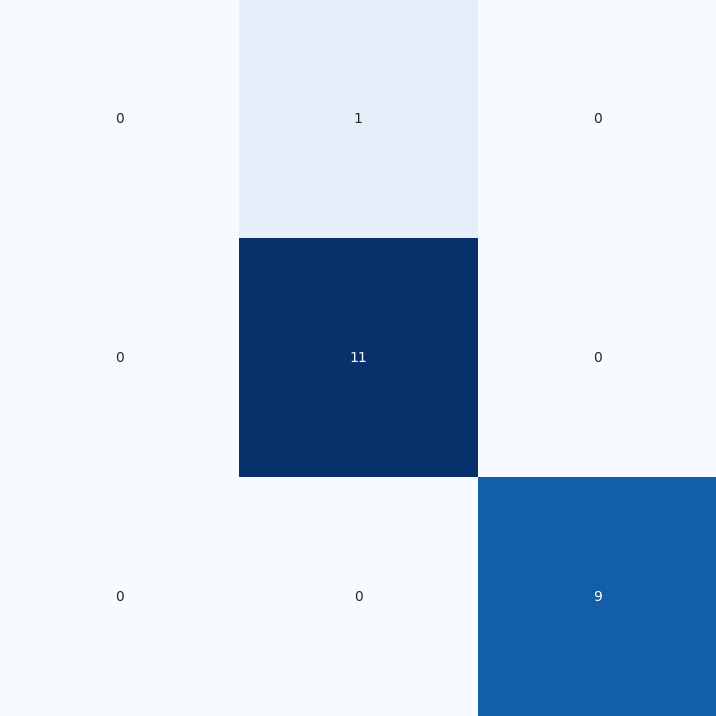
\includegraphics[width=\textwidth]{./class_specific_section/ensemble_plots/ensemble_confusion_matrix_PR.png}
        \caption{Ensemble for PR}
        \label{fig_class:spec_ensemble_pr}
    \end{minipage}
    \hfill
    \begin{minipage}[b]{0.45\textwidth}
        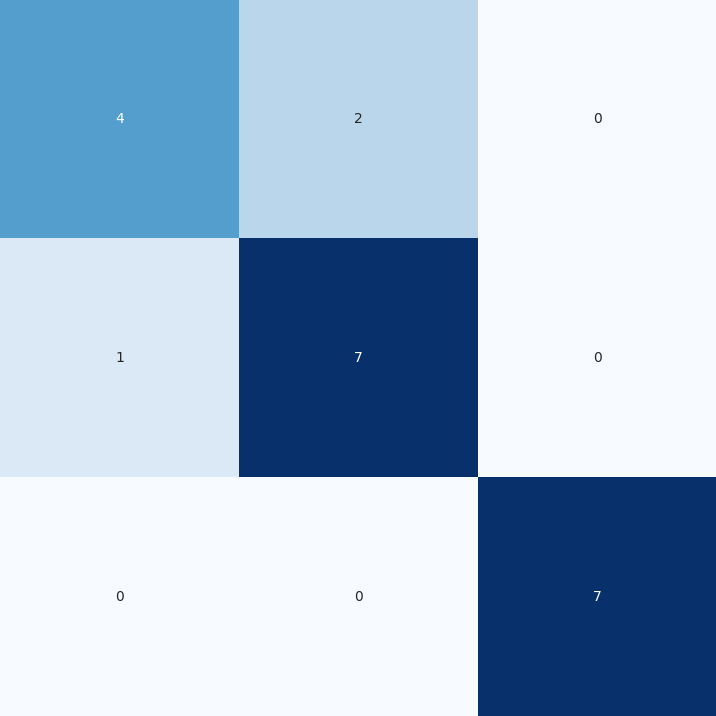
\includegraphics[width=\textwidth]{./class_specific_section/ensemble_plots/ensemble_confusion_matrix_NR.png}
        \caption{Ensemble for NR}
        \label{fig_class:spec_ensemble_nr}
    \end{minipage}
\end{figure}

\begin{figure}[H]
    \centering
    \begin{minipage}[b]{0.45\textwidth}
        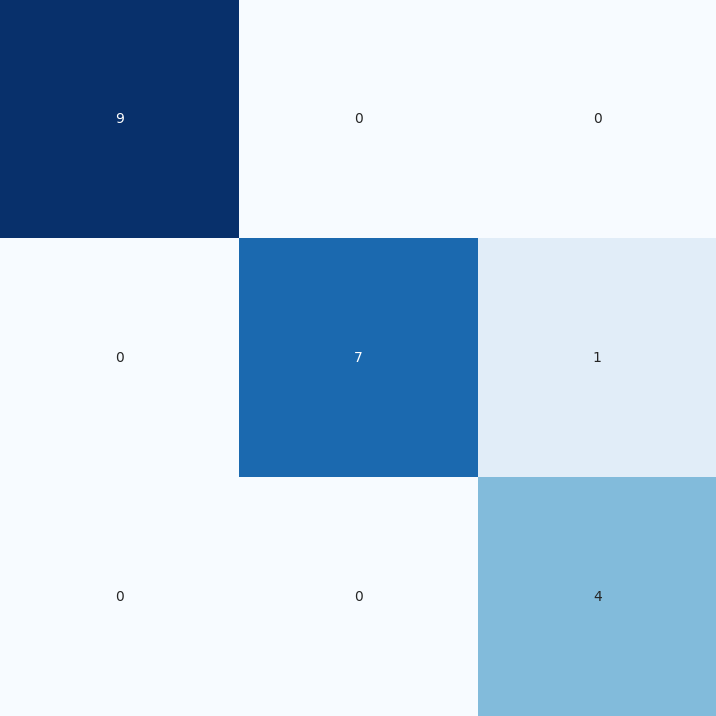
\includegraphics[width=\textwidth]{./class_specific_section/ensemble_plots/ensemble_confusion_matrix_SR.png}
        \caption{Ensemble for SR}
        \label{fig_class:spec_ensemble_sr}
    \end{minipage}
    \hfill
    \begin{minipage}[b]{0.45\textwidth}
        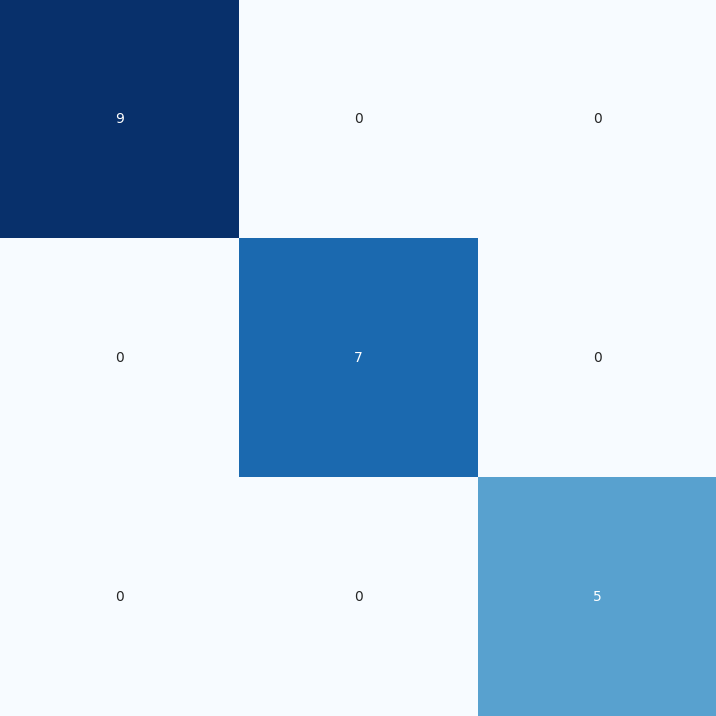
\includegraphics[width=\textwidth]{./class_specific_section/ensemble_plots/ensemble_confusion_matrix_WS.png}
        \caption{Ensemble for WS}
        \label{fig_class:spec_ensemble_ws}
    \end{minipage}
\end{figure}

\begin{figure}[H]
    \centering
    \begin{minipage}[b]{0.45\textwidth}
        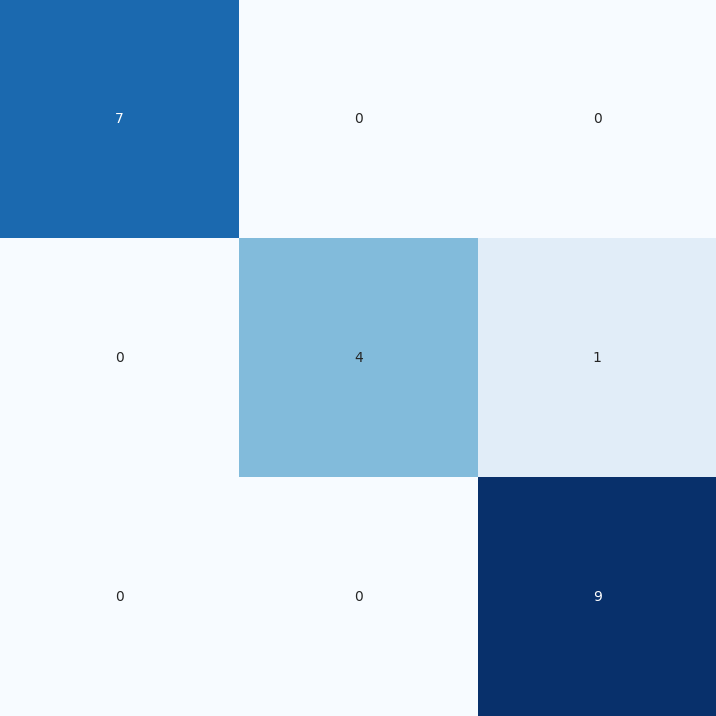
\includegraphics[width=\textwidth]{./class_specific_section/ensemble_plots/ensemble_confusion_matrix_SFST.png}
        \caption{Ensemble for SFST}
        \label{fig_class:spec_ensemble_sfst}
    \end{minipage}
    \hfill
    \begin{minipage}[b]{0.45\textwidth}
        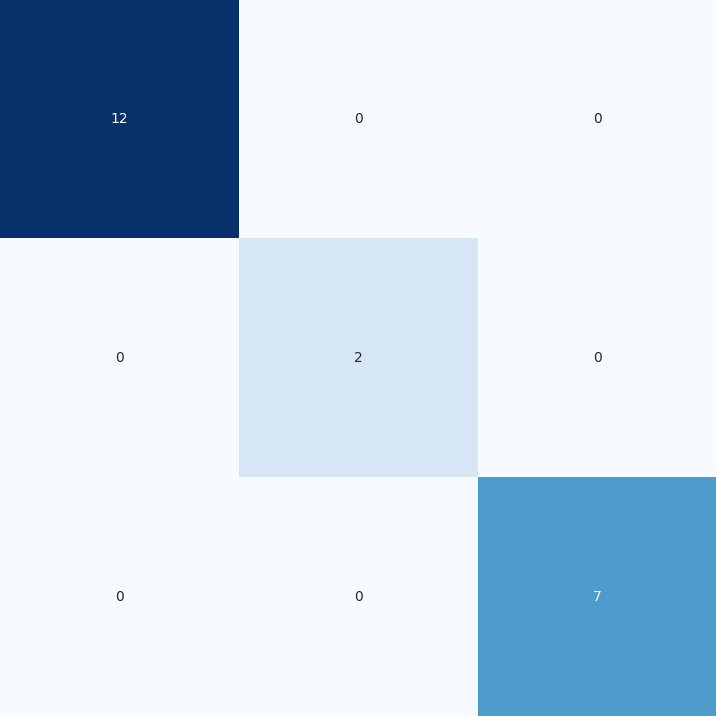
\includegraphics[width=\textwidth]{./class_specific_section/ensemble_plots/ensemble_confusion_matrix_PR_Benefit.png}
        \caption{Ensemble for PR Benefit}
        \label{fig_class:spec_ensemble_pr_benefit}
    \end{minipage}
\end{figure}

\begin{figure}[H]
    \centering
    \begin{minipage}[b]{0.45\textwidth}
        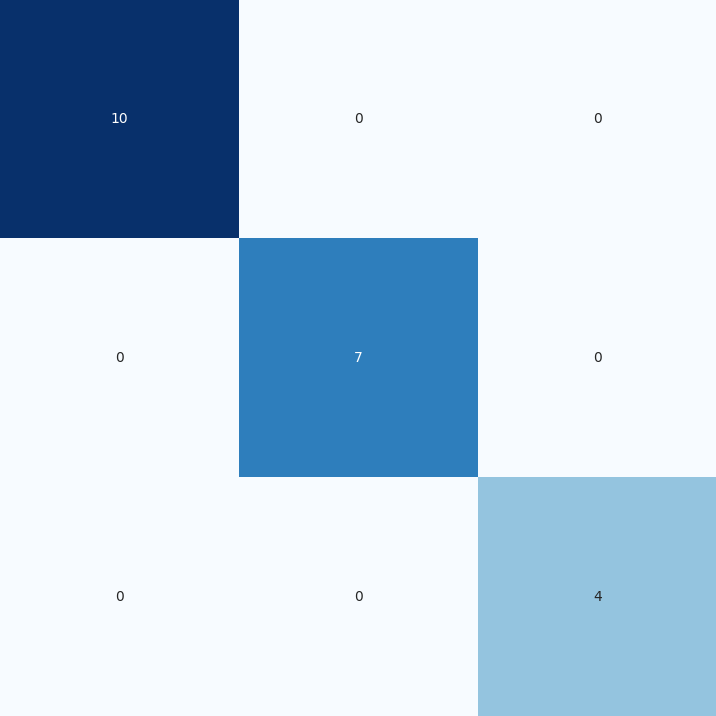
\includegraphics[width=\textwidth]{./class_specific_section/ensemble_plots/ensemble_confusion_matrix_NR_Benefit.png}
        \caption{Ensemble for NR Benefit}
        \label{fig_class:spec_ensemble_nr_benefit}
    \end{minipage}
    \hfill
    \begin{minipage}[b]{0.45\textwidth}
        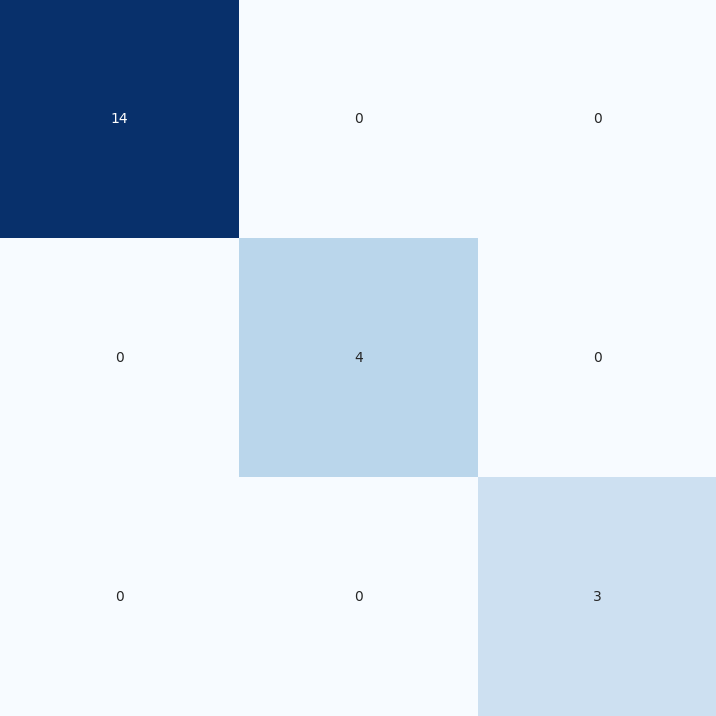
\includegraphics[width=\textwidth]{./class_specific_section/ensemble_plots/ensemble_confusion_matrix_SR_Benefit.png}
        \caption{Ensemble for SR Benefit}
        \label{fig_class:spec_ensemble_sr_benefit}
    \end{minipage}
\end{figure}

\begin{figure}[H]
    \centering
    \begin{minipage}[b]{0.45\textwidth}
        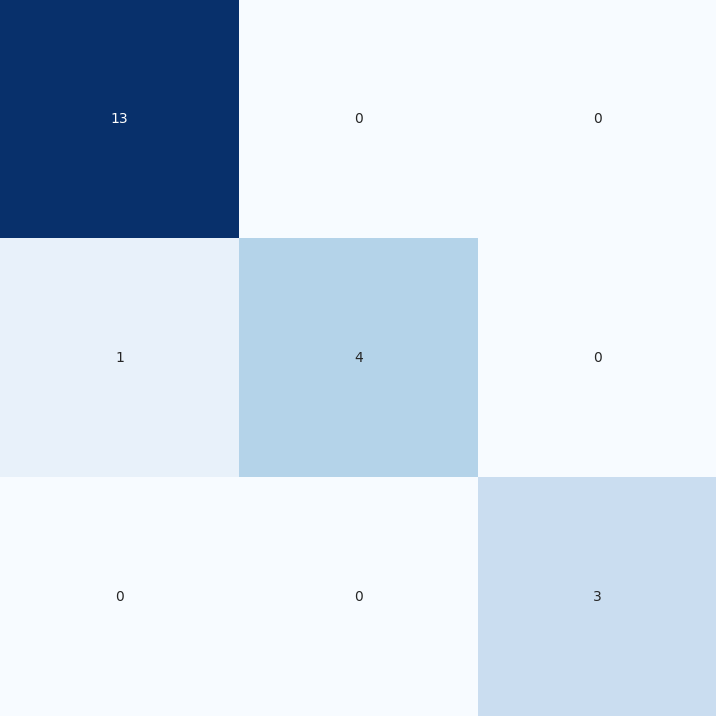
\includegraphics[width=\textwidth]{./class_specific_section/ensemble_plots/ensemble_confusion_matrix_WS_Benefit.png}
        \caption{Ensemble for WS Benefit}
        \label{fig_class:spec_ensemble_ws_benefit}
    \end{minipage}
    \hfill
    \begin{minipage}[b]{0.45\textwidth}
        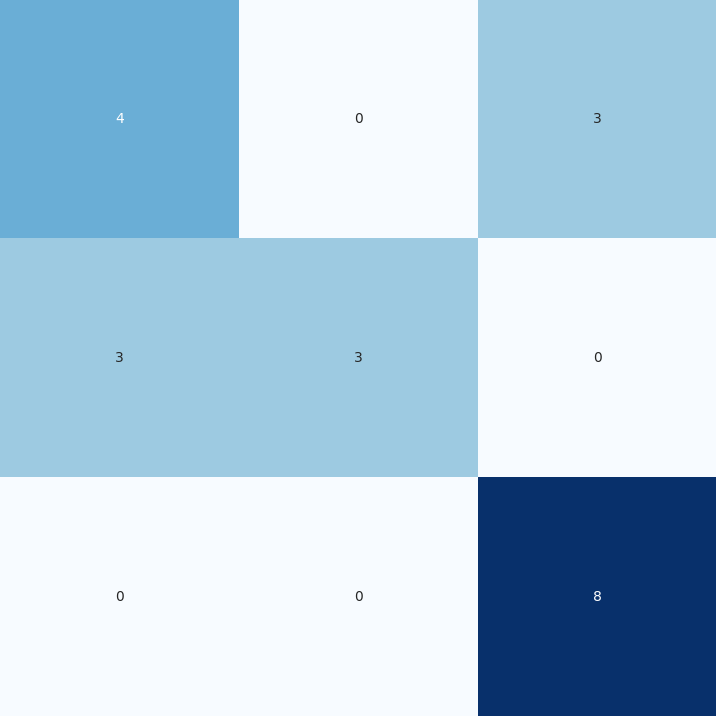
\includegraphics[width=\textwidth]{./class_specific_section/ensemble_plots/ensemble_confusion_matrix_SFST_Benefit.png}
        \caption{Ensemble for SFST Benefit}
        \label{fig_class:spec_ensemble_sfst_benefit}
    \end{minipage}
\end{figure}
\clearpage
\begin{longtable}{|p{2cm}|p{2cm}|p{2cm}|p{8cm}|}
\hline
\textbf{Function} & \textbf{Accuracy} & \textbf{\# Feat.} & \textbf{Selected Features} \\ \hline
\endfirsthead
\hline
\textbf{Function} & \textbf{Accuracy} & \textbf{\# Feat.} & \textbf{Selected Features} \\ \hline
\endhead

PR & 0.9524 & 14 & OF26, F17, F21, F23, F24, F28, F29, F31, F34, F35, F43, F44, F45, F63 \\ \hline
NR & 0.8571 & 23 & OF16, OF22, OF25, OF27, F1, F3b, F3c, F3d, F3e, F3g, F17, F22, F23, F24, F28, F31, F33, F34, F36, F43, F44, F45, F49 \\ \hline
SR & 0.8095 & 6 & OF22, F35, F43, F44, F45, F49 \\ \hline
WS & 1.0000 & 9 & OF22, F3c, F3d, F3e, F28, F43, F44, F45, F49 \\ \hline
SFST & 0.9524 & 2 & F1, F43 \\ \hline
PR Benefit & 0.9524 & 7 & OF19, OF22, OF24, F41, F48, F50, F52 \\ \hline
NR Benefit & 0.9524 & 12 & OF9, OF10, OF19, OF20, OF21, OF22, OF23, OF24, F41, F50, F51, F52 \\ \hline
SR Benefit & 1.0000 & 3 & OF19, OF21, F41 \\ \hline
WS Benefit & 0.9524 & 2 & OF17, OF23 \\ \hline
SFST Benefit & 0.5714 & 2 & OF22, OF28 \\ \hline
\caption{Maximum Accuracy}
\label{tab_class_spec:ensemble_class_acc}
\end{longtable}

% Table for proportionate accuracy
\begin{longtable}{|p{3cm}|p{2cm}|p{2cm}|p{8cm}|}
\hline
\textbf{Function} & \textbf{Accuracy} & \textbf{\# Feat.} & \textbf{Selected Features} \\ \hline
\endfirsthead
\hline
\textbf{Function} & \textbf{Accuracy} & \textbf{\# Feat.} & \textbf{Selected Features} \\ \hline
\endhead

PR & 0.8571 & 2 & F43, F45 \\ \hline
NR & 0.7619 & 2 & F43, F44 \\ \hline
SR & 0.6190 & 2 & F43, F44 \\ \hline
WS & 0.8571 & 2 & F43, F44 \\ \hline
SFST & 0.9524 & 2 & F1, F43 \\ \hline
PR Benefit & 0.9048 & 2 & OF24, F41 \\ \hline
NR Benefit & 0.7619 & 2 & OF10, F41 \\ \hline
SR Benefit & 0.9524 & 2 & OF19, F41 \\ \hline
WS Benefit & 0.9524 & 2 & OF17, OF23 \\ \hline
SFST Benefit & 0.5714 & 2 & OF22, OF28 \\ \hline
\caption{Maximum Proportionate Accuracy}
\label{tab_class_spec:ensemble_prop_class_acc}
\end{longtable}

\clearpage
\begin{figure}[H]
    \centering
    \begin{minipage}[b]{0.45\textwidth}
        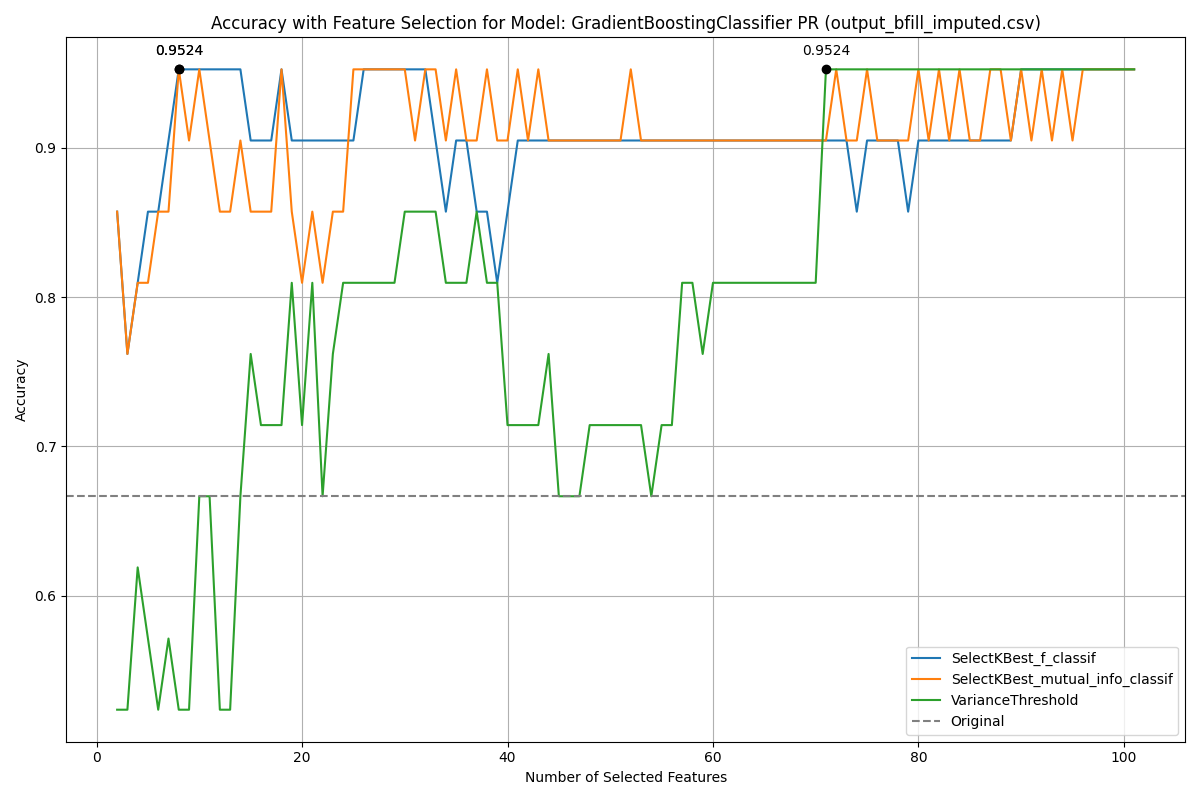
\includegraphics[width=\textwidth]{class_all_section/images/feature_selection_accuracy_plot_output_bfill_imputedcsv_GradientBoostingClassifier_PR.png}
        \caption{PR}
        \label{fig:pr_class}
    \end{minipage}
    \hfill
    \begin{minipage}[b]{0.45\textwidth}
        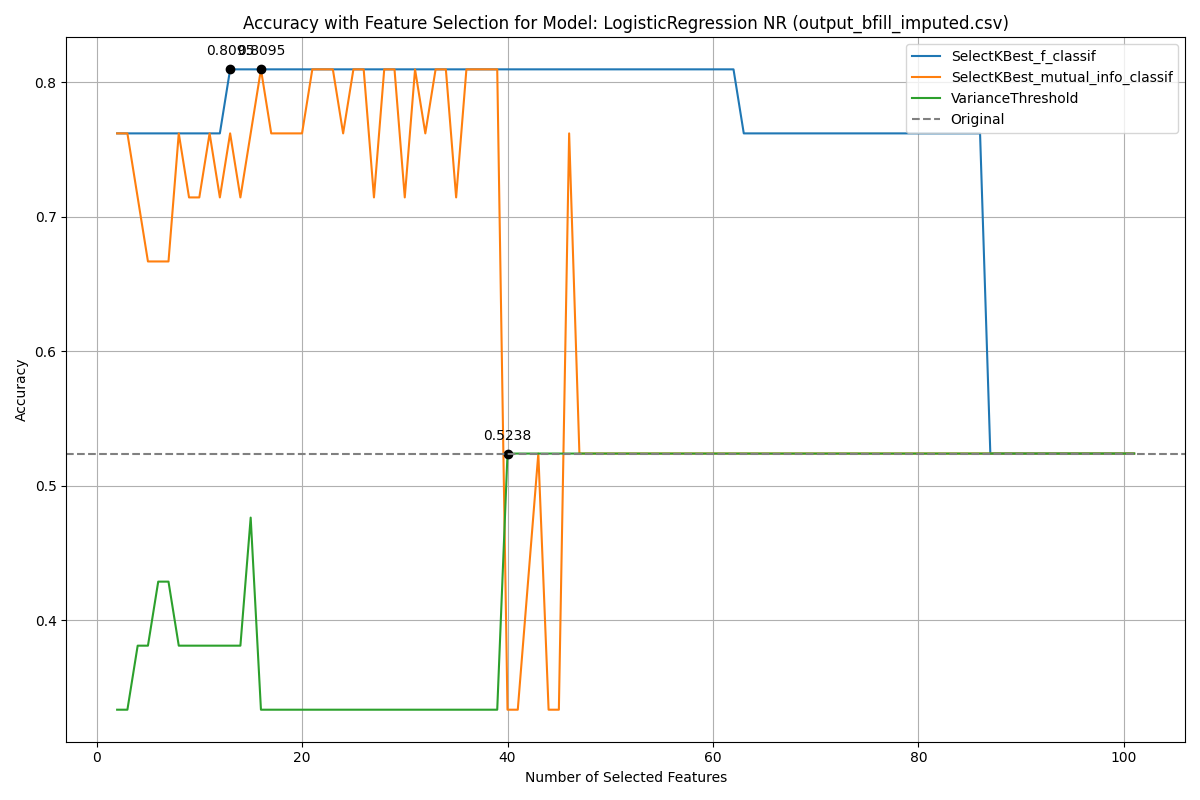
\includegraphics[width=\textwidth]{class_all_section/images/feature_selection_accuracy_plot_output_bfill_imputedcsv_LogisticRegression_NR.png}
        \caption{NR}
        \label{fig:nr_class}
    \end{minipage}
\end{figure}

\begin{figure}[H]
    \centering
    \begin{minipage}[b]{0.45\textwidth}
        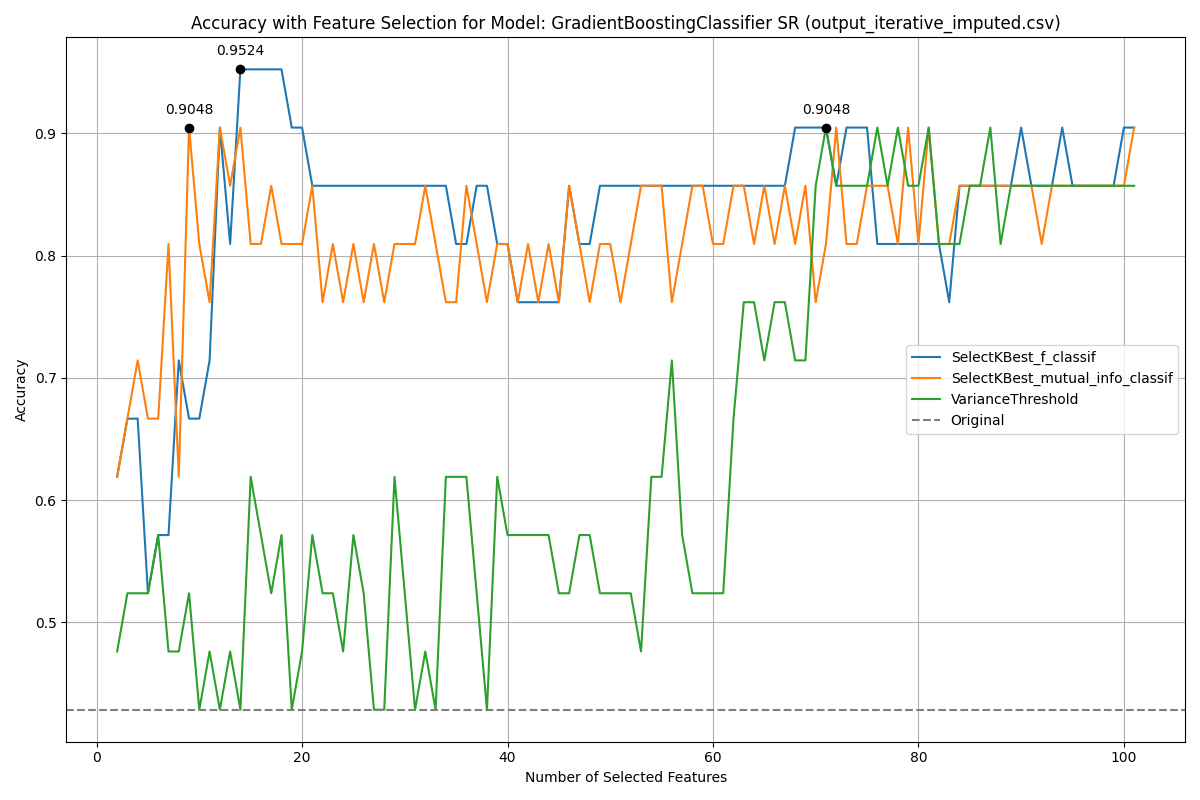
\includegraphics[width=\textwidth]{class_all_section/images/feature_selection_accuracy_plot_output_iterative_imputedcsv_GradientBoostingClassifier_SR.png}
        \caption{SR}
        \label{fig:sr_class}
    \end{minipage}
    \hfill
    \begin{minipage}[b]{0.45\textwidth}
        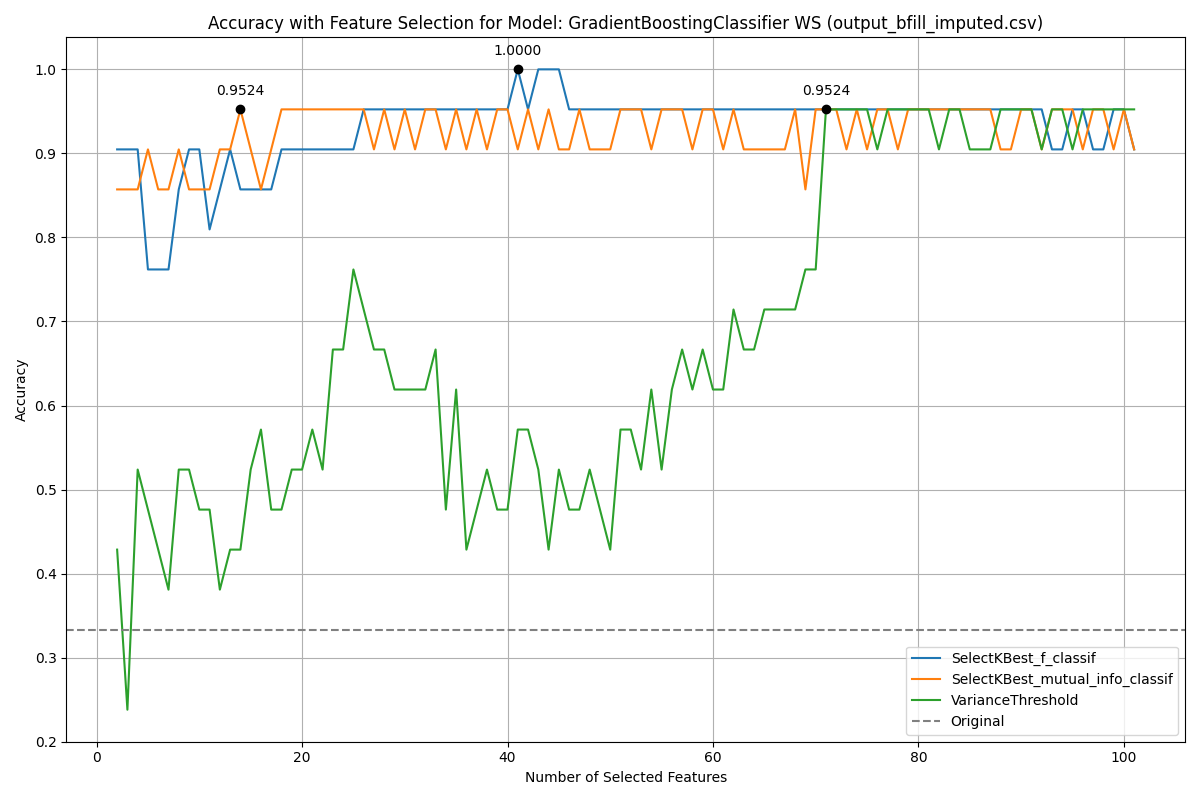
\includegraphics[width=\textwidth]{class_all_section/images/feature_selection_accuracy_plot_output_bfill_imputedcsv_GradientBoostingClassifier_WS.png}
        \caption{WS}
        \label{fig:ws_class}
    \end{minipage}
\end{figure}

\begin{figure}[H]
    \centering
    \begin{minipage}[b]{0.45\textwidth}
        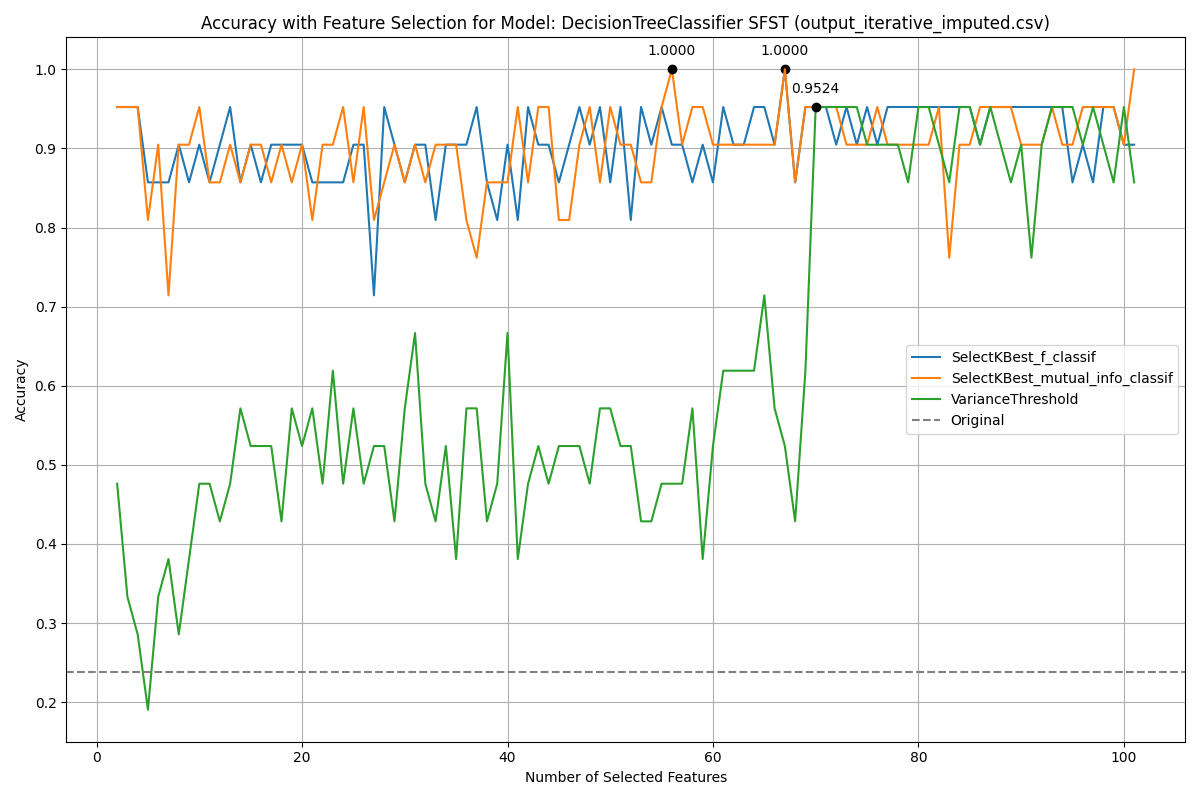
\includegraphics[width=\textwidth]{class_all_section/images/feature_selection_accuracy_plot_output_iterative_imputedcsv_DecisionTreeClassifier_SFST.png}
        \caption{SFST}
        \label{fig:sfst_class}
    \end{minipage}
    \hfill
    \begin{minipage}[b]{0.45\textwidth}
        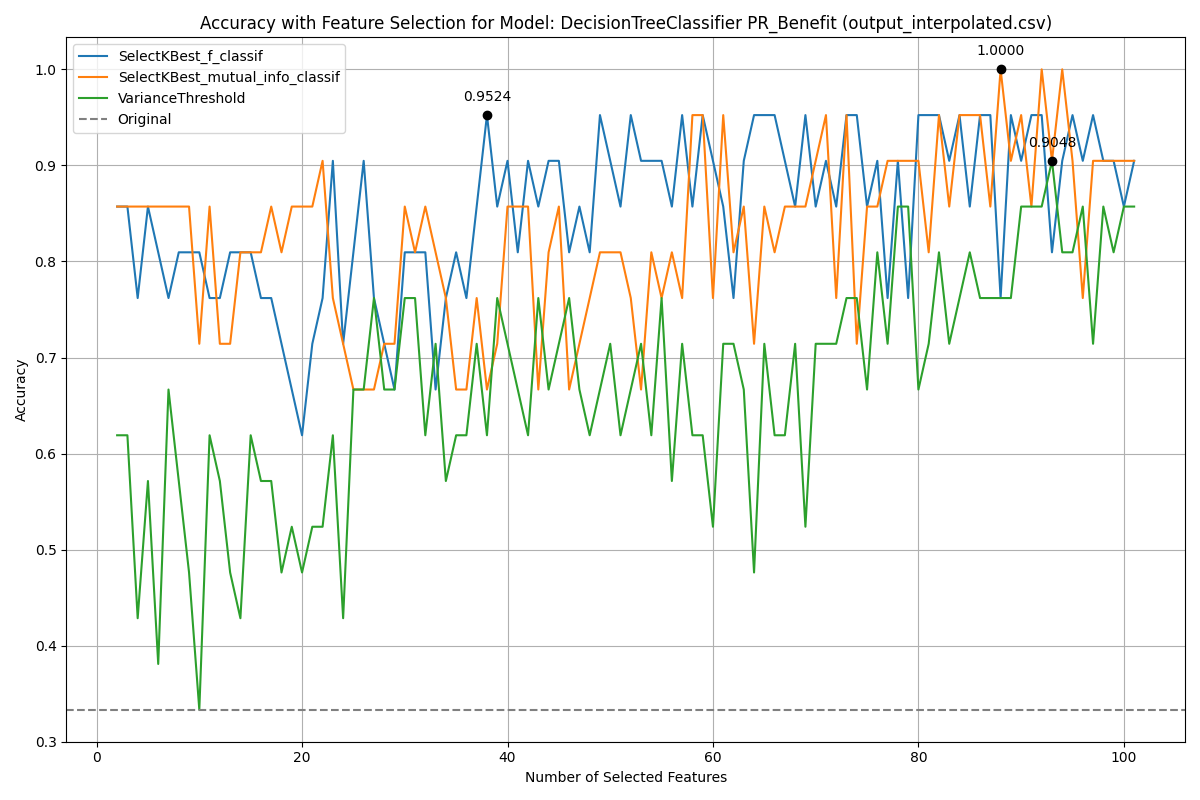
\includegraphics[width=\textwidth]{class_all_section/images/feature_selection_accuracy_plot_output_interpolatedcsv_DecisionTreeClassifier_PR_Benefit.png}
        \caption{PR Benefit}
        \label{fig:pr_ben_class}
    \end{minipage}
\end{figure}

\begin{figure}[H]
    \centering
    \begin{minipage}[b]{0.45\textwidth}
        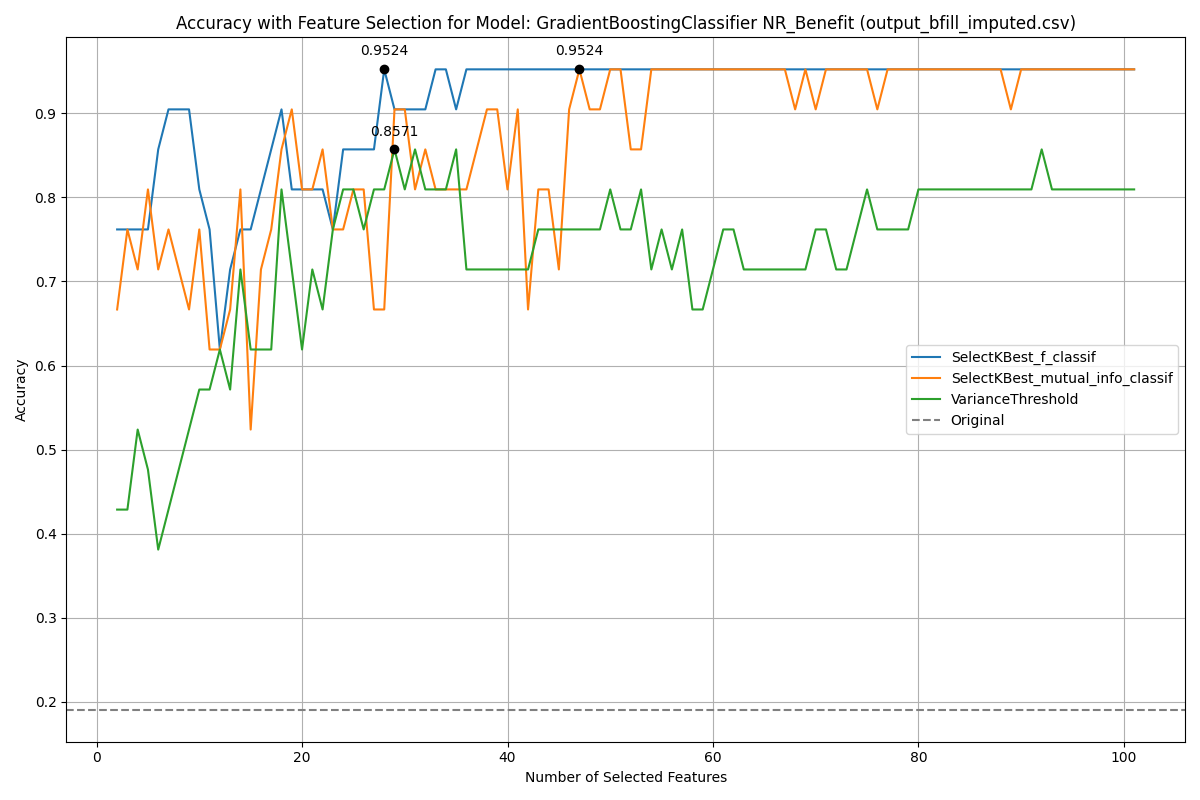
\includegraphics[width=\textwidth]{class_all_section/images/feature_selection_accuracy_plot_output_bfill_imputedcsv_GradientBoostingClassifier_NR_Benefit.png}
        \caption{NR Benefit}
        \label{fig:nr_ben_class}
    \end{minipage}
    \hfill
    \begin{minipage}[b]{0.45\textwidth}
        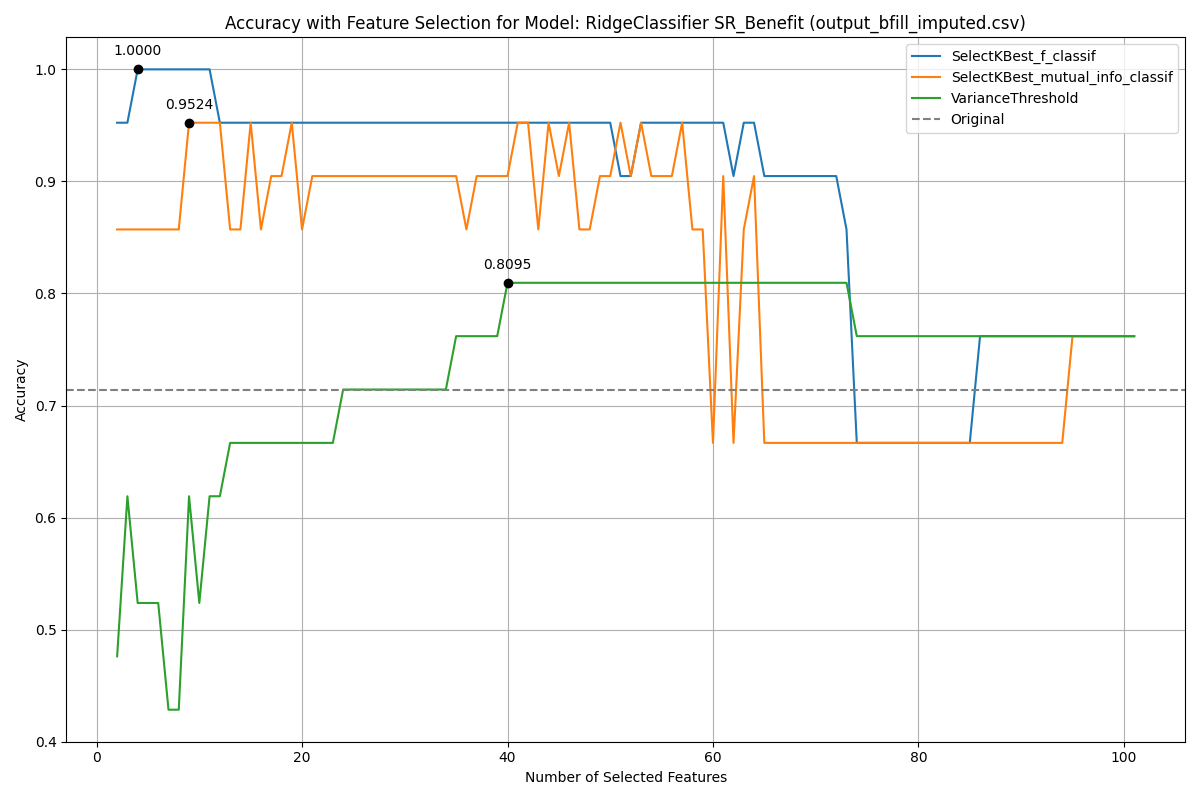
\includegraphics[width=\textwidth]{class_all_section/images/feature_selection_accuracy_plot_output_bfill_imputedcsv_RidgeClassifier_SR_Benefit.png}
        \caption{SR Benefit}
        \label{fig:sr_ben_class}
    \end{minipage}
\end{figure}

\begin{figure}[H]
    \centering
    \begin{minipage}[b]{0.45\textwidth}
        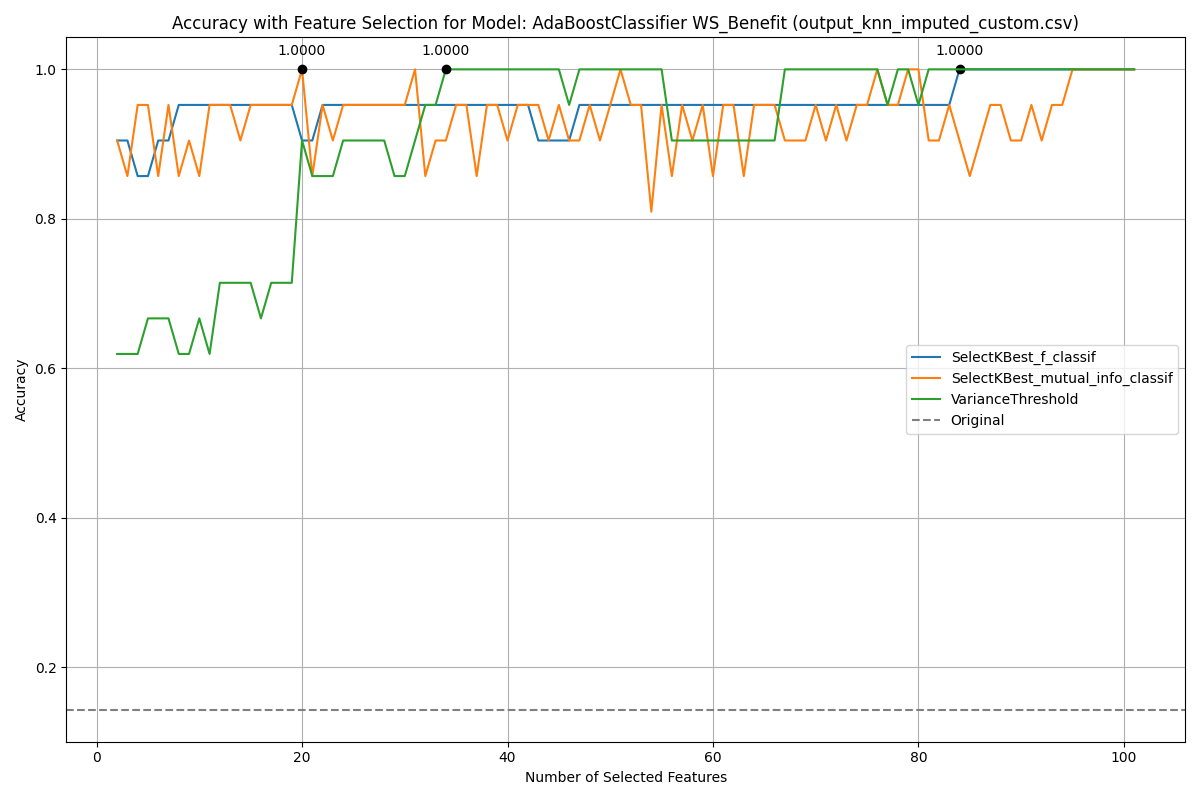
\includegraphics[width=\textwidth]{class_all_section/images/feature_selection_accuracy_plot_output_knn_imputed_customcsv_AdaBoostClassifier_WS_Benefit.png}
        \caption{WS Benefit}
        \label{fig:ws_ben_class}
    \end{minipage}
    \hfill
    \begin{minipage}[b]{0.45\textwidth}
        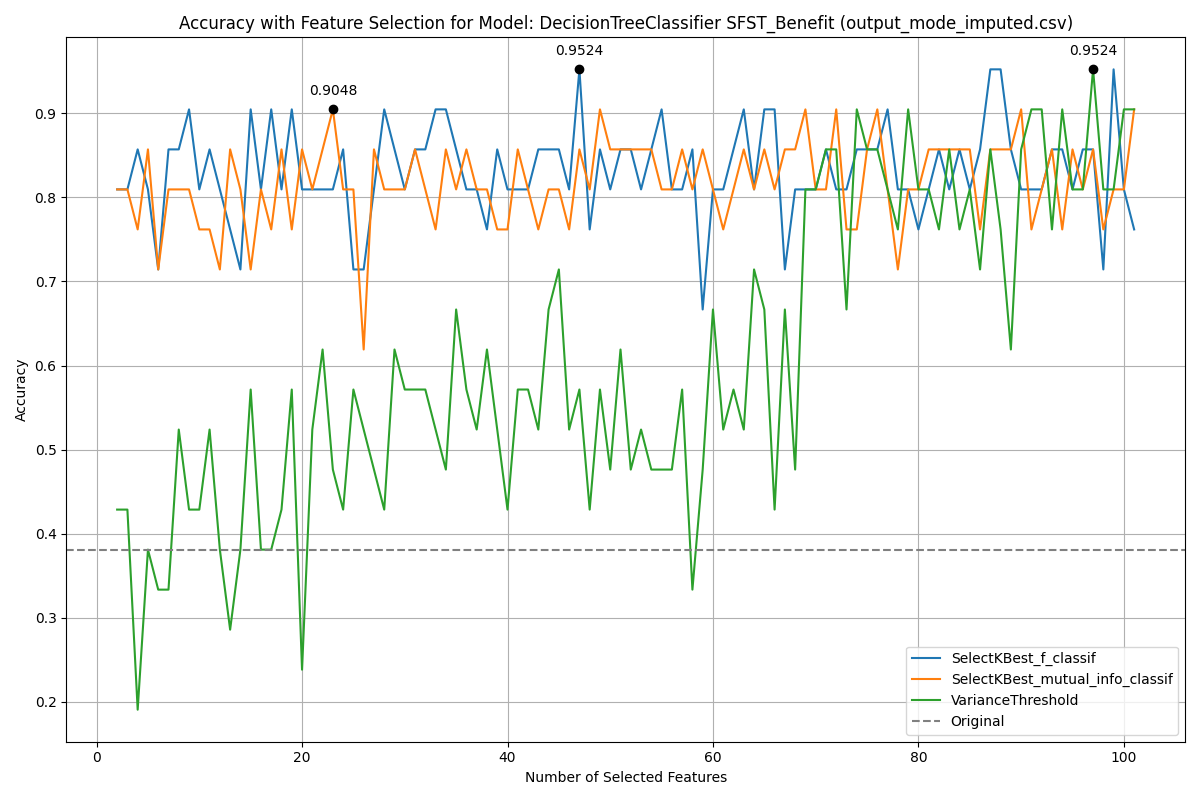
\includegraphics[width=\textwidth]{class_all_section/images/feature_selection_accuracy_plot_output_mode_imputedcsv_DecisionTreeClassifier_SFST_Benefit.png}
        \caption{SFST Benefit}
        \label{fig:sfst_ben_class}
    \end{minipage}
\end{figure}

\clearpage

\subsubsection{Specific Features}
\begin{longtable}{|p{2cm}|p{2cm}|p{2cm}|p{8cm}|}
\hline
\textbf{Function} & \textbf{Accuracy} & \textbf{\# Feat.} & \textbf{Selected Features} \\ \hline
\endfirsthead
\hline
\textbf{Function} & \textbf{Accuracy} & \textbf{\# Feat.} & \textbf{Selected Features} \\ \hline
\endhead

PR & 0.9524 & 14 & OF26, F17, F21, F23, F24, F28, F29, F31, F34, F35, F43, F44, F45, F63 \\ \hline
NR & 0.8571 & 23 & OF16, OF22, OF25, OF27, F1, F3b, F3c, F3d, F3e, F3g, F17, F22, F23, F24, F28, F31, F33, F34, F36, F43, F44, F45, F49 \\ \hline
SR & 0.8095 & 6 & OF22, F35, F43, F44, F45, F49 \\ \hline
WS & 1.0000 & 9 & OF22, F3c, F3d, F3e, F28, F43, F44, F45, F49 \\ \hline
SFST & 0.9524 & 2 & F1, F43 \\ \hline
PR Benefit & 0.9524 & 7 & OF19, OF22, OF24, F41, F48, F50, F52 \\ \hline
NR Benefit & 0.9524 & 12 & OF9, OF10, OF19, OF20, OF21, OF22, OF23, OF24, F41, F50, F51, F52 \\ \hline
SR Benefit & 1.0000 & 3 & OF19, OF21, F41 \\ \hline
WS Benefit & 0.9524 & 2 & OF17, OF23 \\ \hline
SFST Benefit & 0.5714 & 2 & OF22, OF28 \\ \hline
\caption{Maximum Accuracy}
\label{tab_class_spec:ensemble_class_acc}
\end{longtable}

% Table for proportionate accuracy
\begin{longtable}{|p{3cm}|p{2cm}|p{2cm}|p{8cm}|}
\hline
\textbf{Function} & \textbf{Accuracy} & \textbf{\# Feat.} & \textbf{Selected Features} \\ \hline
\endfirsthead
\hline
\textbf{Function} & \textbf{Accuracy} & \textbf{\# Feat.} & \textbf{Selected Features} \\ \hline
\endhead

PR & 0.8571 & 2 & F43, F45 \\ \hline
NR & 0.7619 & 2 & F43, F44 \\ \hline
SR & 0.6190 & 2 & F43, F44 \\ \hline
WS & 0.8571 & 2 & F43, F44 \\ \hline
SFST & 0.9524 & 2 & F1, F43 \\ \hline
PR Benefit & 0.9048 & 2 & OF24, F41 \\ \hline
NR Benefit & 0.7619 & 2 & OF10, F41 \\ \hline
SR Benefit & 0.9524 & 2 & OF19, F41 \\ \hline
WS Benefit & 0.9524 & 2 & OF17, OF23 \\ \hline
SFST Benefit & 0.5714 & 2 & OF22, OF28 \\ \hline
\caption{Maximum Proportionate Accuracy}
\label{tab_class_spec:ensemble_prop_class_acc}
\end{longtable}

\begin{figure}[H]
    \centering
    \begin{minipage}[b]{0.45\textwidth}
        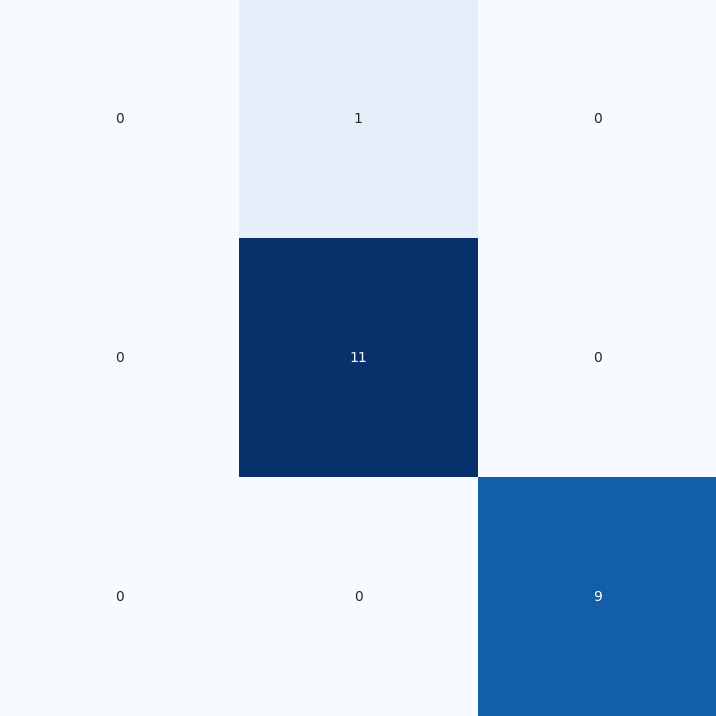
\includegraphics[width=\textwidth]{./class_specific_section/ensemble_plots/ensemble_confusion_matrix_PR.png}
        \caption{Ensemble for PR}
        \label{fig_class:spec_ensemble_pr}
    \end{minipage}
    \hfill
    \begin{minipage}[b]{0.45\textwidth}
        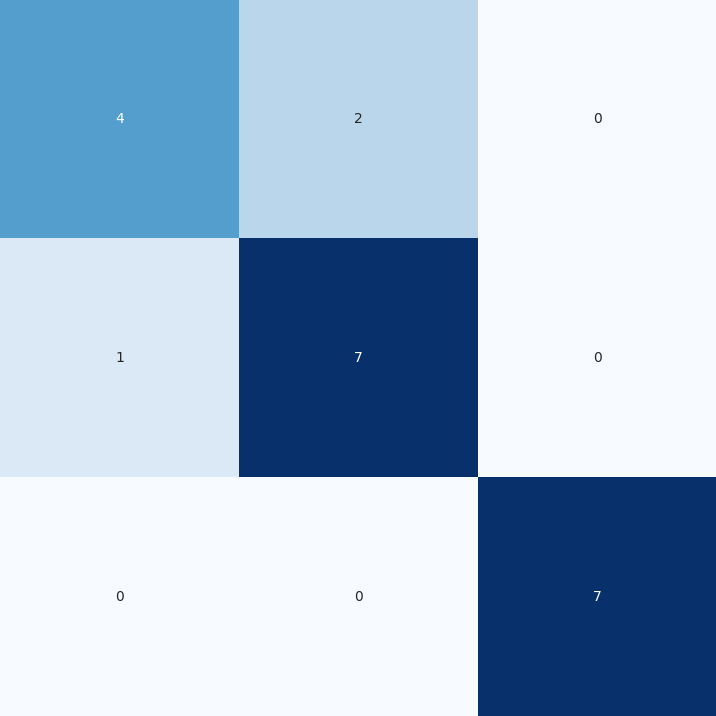
\includegraphics[width=\textwidth]{./class_specific_section/ensemble_plots/ensemble_confusion_matrix_NR.png}
        \caption{Ensemble for NR}
        \label{fig_class:spec_ensemble_nr}
    \end{minipage}
\end{figure}

\begin{figure}[H]
    \centering
    \begin{minipage}[b]{0.45\textwidth}
        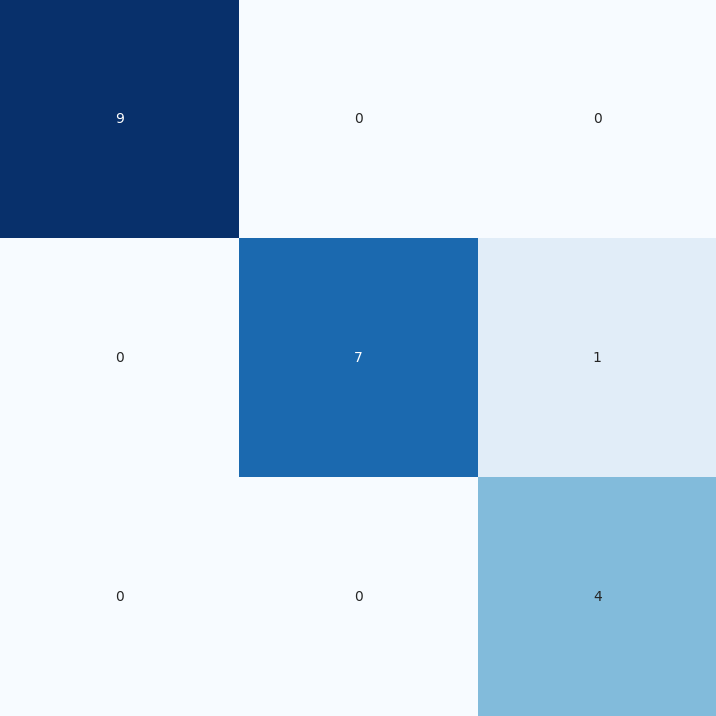
\includegraphics[width=\textwidth]{./class_specific_section/ensemble_plots/ensemble_confusion_matrix_SR.png}
        \caption{Ensemble for SR}
        \label{fig_class:spec_ensemble_sr}
    \end{minipage}
    \hfill
    \begin{minipage}[b]{0.45\textwidth}
        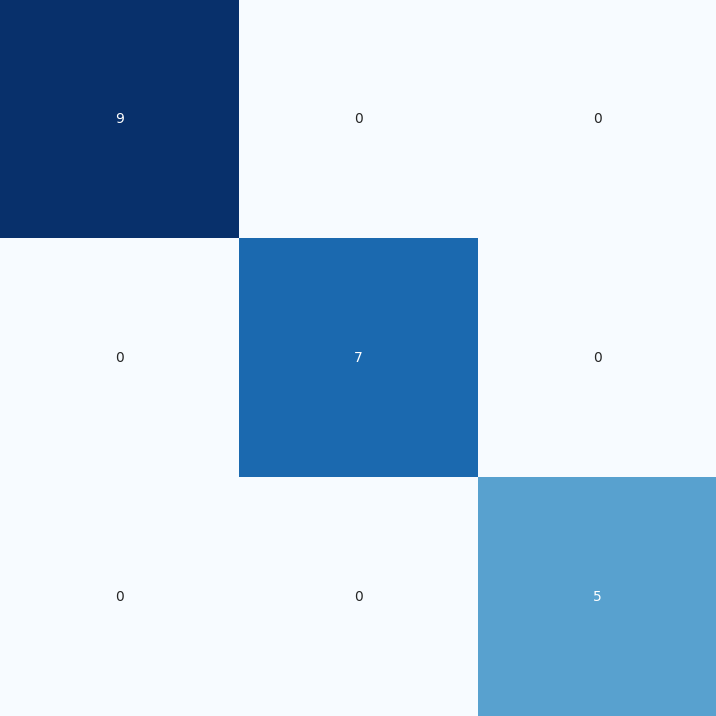
\includegraphics[width=\textwidth]{./class_specific_section/ensemble_plots/ensemble_confusion_matrix_WS.png}
        \caption{Ensemble for WS}
        \label{fig_class:spec_ensemble_ws}
    \end{minipage}
\end{figure}

\begin{figure}[H]
    \centering
    \begin{minipage}[b]{0.45\textwidth}
        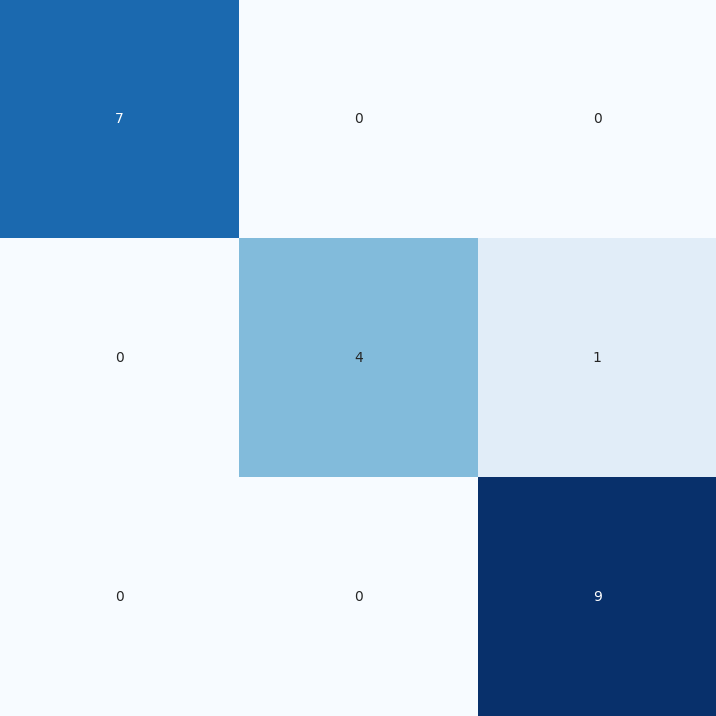
\includegraphics[width=\textwidth]{./class_specific_section/ensemble_plots/ensemble_confusion_matrix_SFST.png}
        \caption{Ensemble for SFST}
        \label{fig_class:spec_ensemble_sfst}
    \end{minipage}
    \hfill
    \begin{minipage}[b]{0.45\textwidth}
        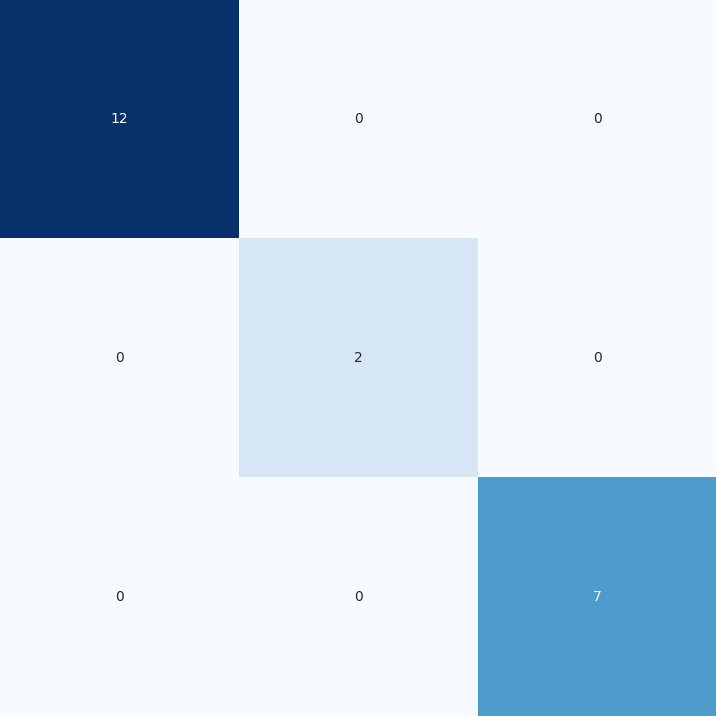
\includegraphics[width=\textwidth]{./class_specific_section/ensemble_plots/ensemble_confusion_matrix_PR_Benefit.png}
        \caption{Ensemble for PR Benefit}
        \label{fig_class:spec_ensemble_pr_benefit}
    \end{minipage}
\end{figure}

\begin{figure}[H]
    \centering
    \begin{minipage}[b]{0.45\textwidth}
        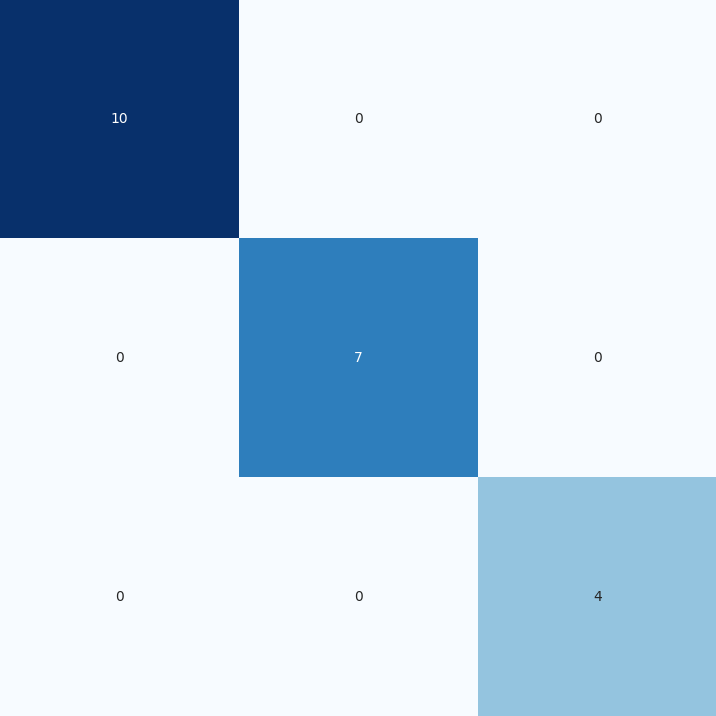
\includegraphics[width=\textwidth]{./class_specific_section/ensemble_plots/ensemble_confusion_matrix_NR_Benefit.png}
        \caption{Ensemble for NR Benefit}
        \label{fig_class:spec_ensemble_nr_benefit}
    \end{minipage}
    \hfill
    \begin{minipage}[b]{0.45\textwidth}
        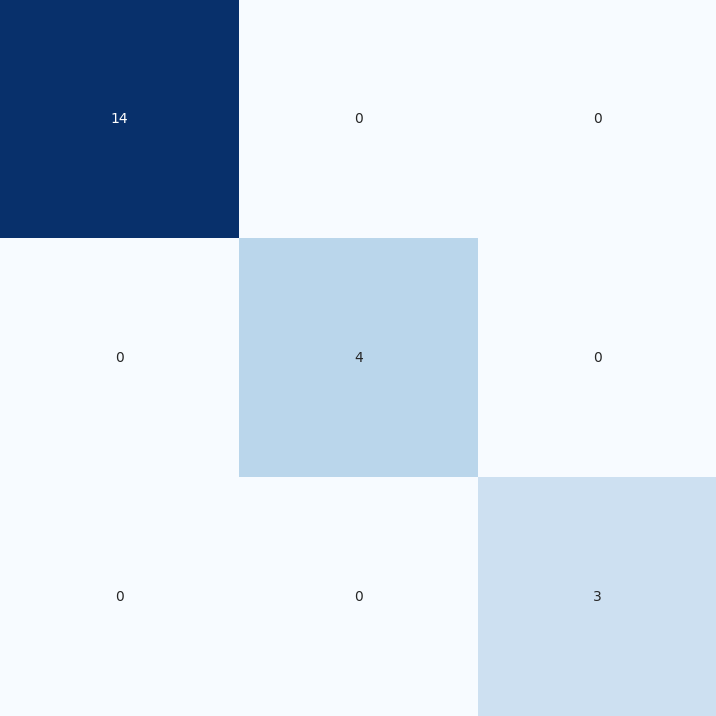
\includegraphics[width=\textwidth]{./class_specific_section/ensemble_plots/ensemble_confusion_matrix_SR_Benefit.png}
        \caption{Ensemble for SR Benefit}
        \label{fig_class:spec_ensemble_sr_benefit}
    \end{minipage}
\end{figure}

\begin{figure}[H]
    \centering
    \begin{minipage}[b]{0.45\textwidth}
        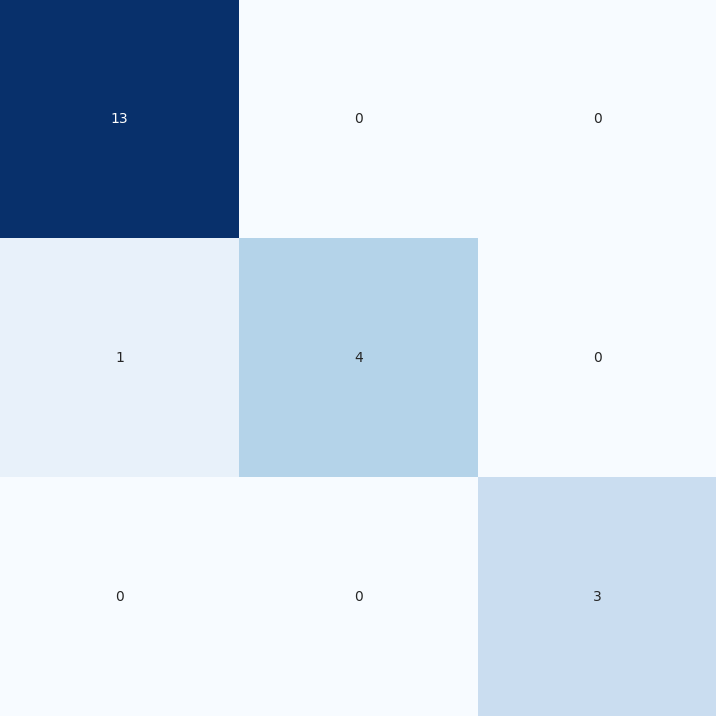
\includegraphics[width=\textwidth]{./class_specific_section/ensemble_plots/ensemble_confusion_matrix_WS_Benefit.png}
        \caption{Ensemble for WS Benefit}
        \label{fig_class:spec_ensemble_ws_benefit}
    \end{minipage}
    \hfill
    \begin{minipage}[b]{0.45\textwidth}
        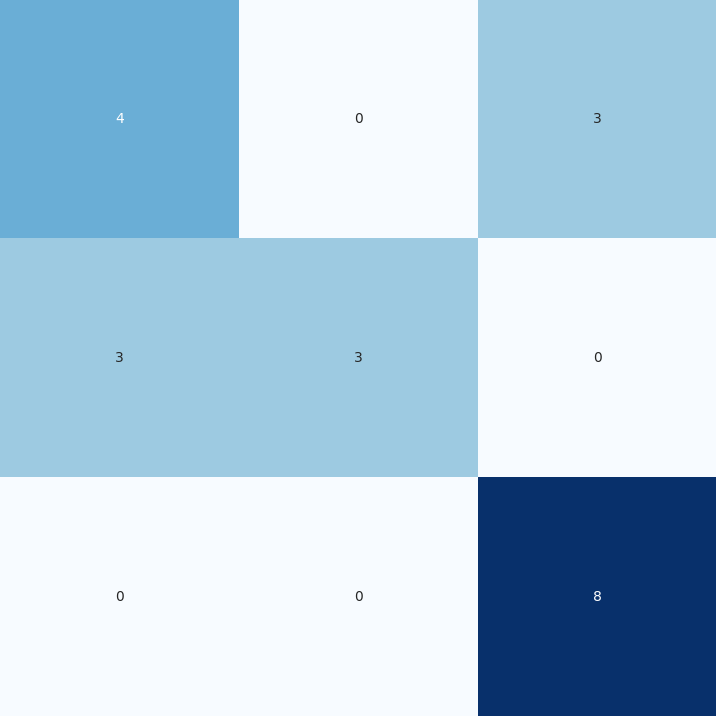
\includegraphics[width=\textwidth]{./class_specific_section/ensemble_plots/ensemble_confusion_matrix_SFST_Benefit.png}
        \caption{Ensemble for SFST Benefit}
        \label{fig_class:spec_ensemble_sfst_benefit}
    \end{minipage}
\end{figure}

\subsubsection{Extra Features}
\begin{longtable}{|p{2cm}|p{2cm}|p{2cm}|p{8cm}|}
\hline
\textbf{Function} & \textbf{Accuracy} & \textbf{\# Feat.} & \textbf{Selected Features} \\ \hline
\endfirsthead
\hline
\textbf{Function} & \textbf{Accuracy} & \textbf{\# Feat.} & \textbf{Selected Features} \\ \hline
\endhead

PR & 0.8571 & 9 & Provincial\_Class, Federal\_Class, Regime, Vegetation\_Type, Vegetation\_Cover, Woody\_Canopy\_Cover, Moss\_Cover, Soil\_Type, Surface\_Water\_Present, Saturation\_Depth, Living\_Moss\_Depth, Organic\_Depth, Hydrogeomorphic\_Class \\ \hline
NR & 0.6667 & 9 & Provincial\_Class, Federal\_Class, Regime, Vegetation\_Type, Vegetation\_Cover, Woody\_Canopy\_Cover, Moss\_Cover, Soil\_Type, Surface\_Water\_Present, Saturation\_Depth, Living\_Moss\_Depth, Organic\_Depth, Hydrogeomorphic\_Class \\ \hline
SR & 0.6190 & 11 & Provincial\_Class, Federal\_Class, Regime, Vegetation\_Type, Vegetation\_Cover, Moss\_Cover, Phragmites, Soil\_Type, Surface\_Water\_Present, Living\_Moss\_Depth, Organic\_Depth \\ \hline
WS & 0.8095 & 5 & Provincial\_Class, Federal\_Class, Regime, Vegetation\_Type, Hydrogeomorphic\_Class \\ \hline
SFST & 0.7143 & 2 & Provincial\_Class, Federal\_Class \\ \hline
PR Benefit & 0.7619 & 6 & Provincial\_Class, Federal\_Class, Regime, Vegetation\_Type, Vegetation\_Cover, Woody\_Canopy\_Cover, Moss\_Cover, Soil\_Type, Surface\_Water\_Present, Saturation\_Depth, Living\_Moss\_Depth, Organic\_Depth, Hydrogeomorphic\_Class \\ \hline
NR Benefit & 0.6667 & 5 & Provincial\_Class, Federal\_Class, Regime, Moss\_Cover, Living\_Moss\_Depth \\ \hline
SR Benefit & 0.8095 & 6 & Provincial\_Class, Federal\_Class, Regime, Vegetation\_Type, Vegetation\_Cover, Woody\_Canopy\_Cover, Moss\_Cover, Soil\_Type, Surface\_Water\_Present, Saturation\_Depth, Living\_Moss\_Depth, Organic\_Depth, Hydrogeomorphic\_Class \\ \hline
WS Benefit & 0.7619 & 9 & Provincial\_Class, Federal\_Class, Regime, Woody\_Canopy\_Cover, Phragmites, Surface\_Water\_Present, Living\_Moss\_Depth, Organic\_Depth, Hydrogeomorphic\_Class \\ \hline
SFST Benefit & 0.6667 & 5 & Provincial\_Class, Federal\_Class, Moss\_Cover, Surface\_Water\_Present, Hydrogeomorphic\_Class \\ \hline

\caption{Maximum Accuracy}
\label{tab_class_xtra:ensemble_class_acc}
\end{longtable}


\begin{longtable}{|p{3cm}|p{2cm}|p{2cm}|p{8cm}|}
\hline
\textbf{Function} & \textbf{Accuracy} & \textbf{\# Feat.} & \textbf{Selected Features} \\ \hline
\endfirsthead
\hline
\textbf{Function} & \textbf{Accuracy} & \textbf{\# Feat.} & \textbf{Selected Features} \\ \hline
\endhead

PR & 0.7619 & 2 & Provincial\_Class, Moss\_Cover \\ \hline
NR & 0.5714 & 2 & Provincial\_Class, Federal\_Class \\ \hline
SR & 0.4286 & 2 & Provincial\_Class, Hydrogeomorphic\_Class \\ \hline
WS & 0.5238 & 2 & Provincial\_Class, Federal\_Class \\ \hline
SFST & 0.7143 & 2 & Provincial\_Class, Federal\_Class \\ \hline
PR Benefit & 0.7143 & 2 & Provincial\_Class, Federal\_Class \\ \hline
NR Benefit & 0.5714 & 2 & Provincial\_Class, Federal\_Class \\ \hline
SR Benefit & 0.7143 & 2 & Provincial\_Class, Moss\_Cover \\ \hline
WS Benefit & 0.6190 & 2 & Moss\_Cover, Living\_Moss\_Depth \\ \hline
SFST Benefit & 0.5714 & 2 & Provincial\_Class, Federal\_Class \\ \hline

\caption{Maximum Proportionate Accuracy}
\label{tab_class_xtra:ensemble_prop_class_acc}
\end{longtable}

\begin{longtable}{|p{2cm}|p{2cm}|p{2cm}|p{2cm}|p{6cm}|}
\hline
\textbf{Function} & \textbf{Best Acc.} & \textbf{2nd Best Acc.} & \textbf{Ensemble Learning Acc.} & \textbf{Features Used} \\ \hline
PR & 85.71\% & 85.71\% & 80.95\% & Federal Class, Hydrogeomorphic Class, Living Moss Depth, Moss Cover, Organic Depth, Provincial Class, Regime, Saturation Depth, Soil Type, Surface Water Present, Vegetation Cover, Vegetation Type, Woody Canopy Cover \\ \hline
NR & 66.67\% & 66.67\% & 61.90\% & Federal Class, Hydrogeomorphic Class, Living Moss Depth, Moss Cover, Organic Depth, Provincial Class, Regime, Saturation Depth, Soil Type, Surface Water Present, Vegetation Cover, Vegetation Type, Woody Canopy Cover \\ \hline
SR & 57.14\% & 52.38\% & 66.67\% & Federal Class, Hydrogeomorphic Class, Living Moss Depth, Moss Cover, Organic Depth, Provincial Class, Regime, Saturation Depth, Soil Type, Surface Water Present, Vegetation Cover, Vegetation Type, Woody Canopy Cover \\ \hline
WS & 80.95\% & 80.95\% & 80.95\% & Federal Class, Hydrogeomorphic Class, Living Moss Depth, Moss Cover, Organic Depth, Provincial Class, Regime, Saturation Depth, Soil Type, Surface Water Present, Vegetation Cover, Vegetation Type, Woody Canopy Cover \\ \hline
SFST & 71.43\% & 71.43\% & 76.19\% & Federal Class, Hydrogeomorphic Class, Living Moss Depth, Moss Cover, Organic Depth, Provincial Class, Regime, Saturation Depth, Soil Type, Surface Water Present, Vegetation Cover, Vegetation Type, Woody Canopy Cover \\ \hline
PR Benefit & 76.19\% & 76.19\% & 71.43\% & Federal Class, Hydrogeomorphic Class, Living Moss Depth, Moss Cover, Organic Depth, Phragmites, Provincial Class, Regime, Saturation Depth, Soil Type, Surface Water Present, Vegetation Cover, Vegetation Type, Woody Canopy Cover \\ \hline
NR Benefit & 66.67\% & 66.67\% & 66.67\% & Federal Class, Hydrogeomorphic Class, Living Moss Depth, Moss Cover, Organic Depth, Provincial Class, Regime, Saturation Depth, Soil Type, Surface Water Present, Vegetation Cover, Vegetation Type, Woody Canopy Cover \\ \hline
SR Benefit & 80.95\% & 76.19\% & 76.19\% & Federal Class, Hydrogeomorphic Class, Living Moss Depth, Moss Cover, Organic Depth, Provincial Class, Regime, Saturation Depth, Soil Type, Surface Water Present, Vegetation Cover, Vegetation Type, Woody Canopy Cover \\ \hline
WS Benefit & 76.19\% & 71.43\% & 66.67\% & Federal Class, Hydrogeomorphic Class, Living Moss Depth, Moss Cover, Organic Depth, Phragmites, Provincial Class, Regime, Saturation Depth, Soil Type, Surface Water Present, Vegetation Cover, Vegetation Type, Woody Canopy Cover \\ \hline
SFST Benefit & 66.67\% & 61.90\% & 61.90\% & Federal Class, Hydrogeomorphic Class, Living Moss Depth, Moss Cover, Organic Depth, Provincial Class, Regime, Saturation Depth, Soil Type, Surface Water Present, Vegetation Cover, Vegetation Type, Woody Canopy Cover \\ \hline
\caption{Ensemble Learning Accuracy}
\label{tab_class_xtra:ensemble_reduction}
\end{longtable}
\clearpage
\subsubsection{Specific + Extra Features}
\begin{longtable}{|p{2cm}|p{2cm}|p{2cm}|p{8cm}|}
\hline
\textbf{Function} & \textbf{Accuracy} & \textbf{\# Feat.} & \textbf{Selected Features} \\ \hline
\endfirsthead
\hline
\textbf{Function} & \textbf{Accuracy} & \textbf{\# Feat.} & \textbf{Selected Features} \\ \hline
\endhead

PR & 0.8571 & 9 & Provincial\_Class, Federal\_Class, Regime, Vegetation\_Type, Vegetation\_Cover, Woody\_Canopy\_Cover, Moss\_Cover, Soil\_Type, Surface\_Water\_Present, Saturation\_Depth, Living\_Moss\_Depth, Organic\_Depth, Hydrogeomorphic\_Class \\ \hline
NR & 0.6667 & 9 & Provincial\_Class, Federal\_Class, Regime, Vegetation\_Type, Vegetation\_Cover, Woody\_Canopy\_Cover, Moss\_Cover, Soil\_Type, Surface\_Water\_Present, Saturation\_Depth, Living\_Moss\_Depth, Organic\_Depth, Hydrogeomorphic\_Class \\ \hline
SR & 0.6190 & 11 & Provincial\_Class, Federal\_Class, Regime, Vegetation\_Type, Vegetation\_Cover, Moss\_Cover, Phragmites, Soil\_Type, Surface\_Water\_Present, Living\_Moss\_Depth, Organic\_Depth \\ \hline
WS & 0.8095 & 5 & Provincial\_Class, Federal\_Class, Regime, Vegetation\_Type, Hydrogeomorphic\_Class \\ \hline
SFST & 0.7143 & 2 & Provincial\_Class, Federal\_Class \\ \hline
PR Benefit & 0.7619 & 6 & Provincial\_Class, Federal\_Class, Regime, Vegetation\_Type, Vegetation\_Cover, Woody\_Canopy\_Cover, Moss\_Cover, Soil\_Type, Surface\_Water\_Present, Saturation\_Depth, Living\_Moss\_Depth, Organic\_Depth, Hydrogeomorphic\_Class \\ \hline
NR Benefit & 0.6667 & 5 & Provincial\_Class, Federal\_Class, Regime, Moss\_Cover, Living\_Moss\_Depth \\ \hline
SR Benefit & 0.8095 & 6 & Provincial\_Class, Federal\_Class, Regime, Vegetation\_Type, Vegetation\_Cover, Woody\_Canopy\_Cover, Moss\_Cover, Soil\_Type, Surface\_Water\_Present, Saturation\_Depth, Living\_Moss\_Depth, Organic\_Depth, Hydrogeomorphic\_Class \\ \hline
WS Benefit & 0.7619 & 9 & Provincial\_Class, Federal\_Class, Regime, Woody\_Canopy\_Cover, Phragmites, Surface\_Water\_Present, Living\_Moss\_Depth, Organic\_Depth, Hydrogeomorphic\_Class \\ \hline
SFST Benefit & 0.6667 & 5 & Provincial\_Class, Federal\_Class, Moss\_Cover, Surface\_Water\_Present, Hydrogeomorphic\_Class \\ \hline

\caption{Maximum Accuracy}
\label{tab_class_xtra:ensemble_class_acc}
\end{longtable}


\begin{longtable}{|p{3cm}|p{2cm}|p{2cm}|p{8cm}|}
\hline
\textbf{Function} & \textbf{Accuracy} & \textbf{\# Feat.} & \textbf{Selected Features} \\ \hline
\endfirsthead
\hline
\textbf{Function} & \textbf{Accuracy} & \textbf{\# Feat.} & \textbf{Selected Features} \\ \hline
\endhead

PR & 0.7619 & 2 & Provincial\_Class, Moss\_Cover \\ \hline
NR & 0.5714 & 2 & Provincial\_Class, Federal\_Class \\ \hline
SR & 0.4286 & 2 & Provincial\_Class, Hydrogeomorphic\_Class \\ \hline
WS & 0.5238 & 2 & Provincial\_Class, Federal\_Class \\ \hline
SFST & 0.7143 & 2 & Provincial\_Class, Federal\_Class \\ \hline
PR Benefit & 0.7143 & 2 & Provincial\_Class, Federal\_Class \\ \hline
NR Benefit & 0.5714 & 2 & Provincial\_Class, Federal\_Class \\ \hline
SR Benefit & 0.7143 & 2 & Provincial\_Class, Moss\_Cover \\ \hline
WS Benefit & 0.6190 & 2 & Moss\_Cover, Living\_Moss\_Depth \\ \hline
SFST Benefit & 0.5714 & 2 & Provincial\_Class, Federal\_Class \\ \hline

\caption{Maximum Proportionate Accuracy}
\label{tab_class_xtra:ensemble_prop_class_acc}
\end{longtable}

\begin{figure}[H]
    \centering
    \begin{minipage}[b]{0.45\textwidth}
        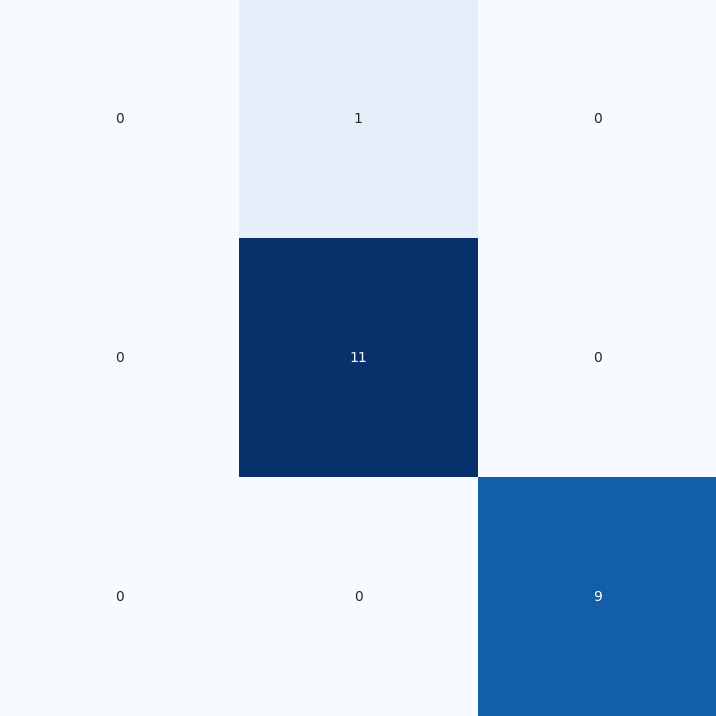
\includegraphics[width=\textwidth]{./class_specific_section/ensemble_plots/ensemble_confusion_matrix_PR.png}
        \caption{Ensemble for PR}
        \label{fig_class:spec_ensemble_pr}
    \end{minipage}
    \hfill
    \begin{minipage}[b]{0.45\textwidth}
        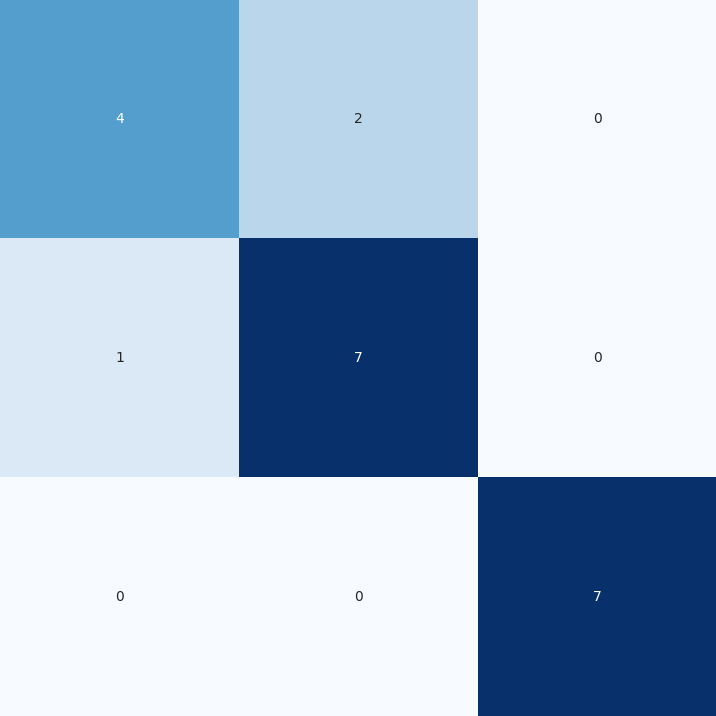
\includegraphics[width=\textwidth]{./class_specific_section/ensemble_plots/ensemble_confusion_matrix_NR.png}
        \caption{Ensemble for NR}
        \label{fig_class:spec_ensemble_nr}
    \end{minipage}
\end{figure}

\begin{figure}[H]
    \centering
    \begin{minipage}[b]{0.45\textwidth}
        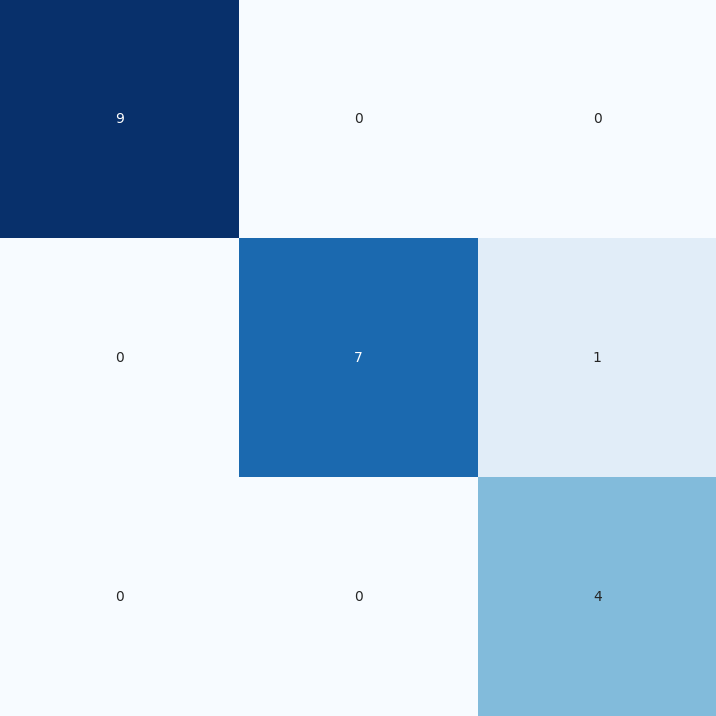
\includegraphics[width=\textwidth]{./class_specific_section/ensemble_plots/ensemble_confusion_matrix_SR.png}
        \caption{Ensemble for SR}
        \label{fig_class:spec_ensemble_sr}
    \end{minipage}
    \hfill
    \begin{minipage}[b]{0.45\textwidth}
        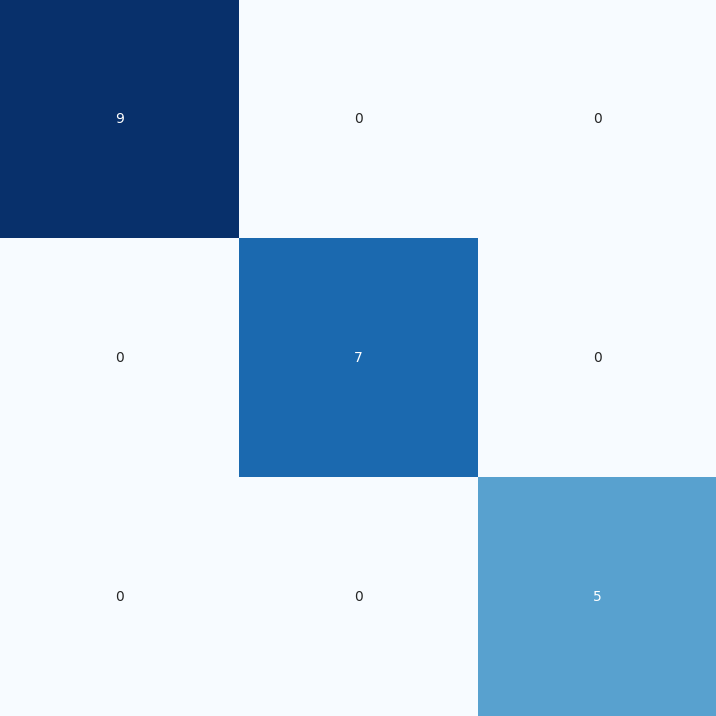
\includegraphics[width=\textwidth]{./class_specific_section/ensemble_plots/ensemble_confusion_matrix_WS.png}
        \caption{Ensemble for WS}
        \label{fig_class:spec_ensemble_ws}
    \end{minipage}
\end{figure}

\begin{figure}[H]
    \centering
    \begin{minipage}[b]{0.45\textwidth}
        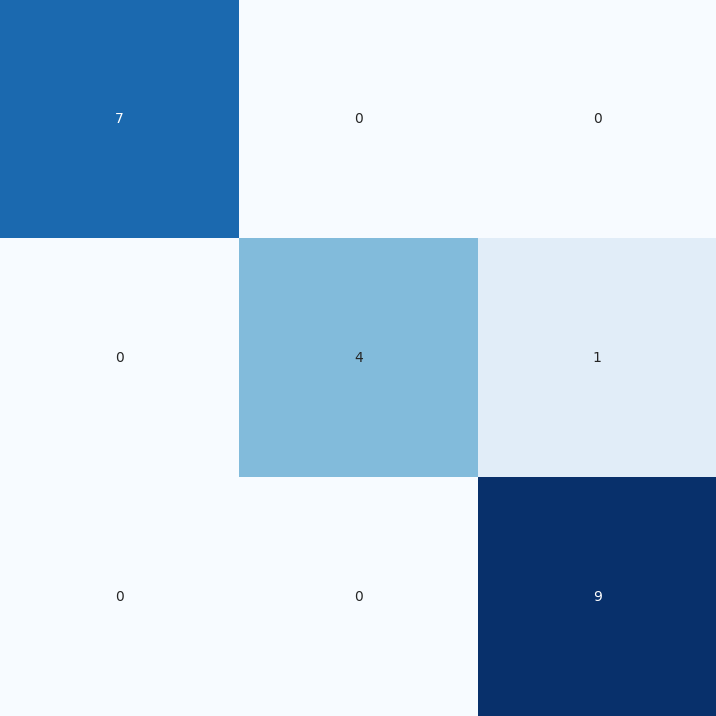
\includegraphics[width=\textwidth]{./class_specific_section/ensemble_plots/ensemble_confusion_matrix_SFST.png}
        \caption{Ensemble for SFST}
        \label{fig_class:spec_ensemble_sfst}
    \end{minipage}
    \hfill
    \begin{minipage}[b]{0.45\textwidth}
        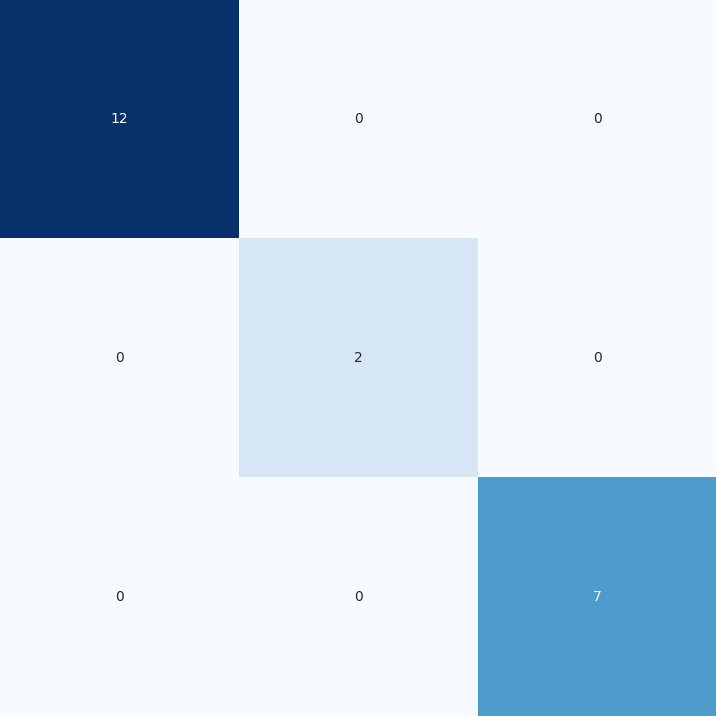
\includegraphics[width=\textwidth]{./class_specific_section/ensemble_plots/ensemble_confusion_matrix_PR_Benefit.png}
        \caption{Ensemble for PR Benefit}
        \label{fig_class:spec_ensemble_pr_benefit}
    \end{minipage}
\end{figure}

\begin{figure}[H]
    \centering
    \begin{minipage}[b]{0.45\textwidth}
        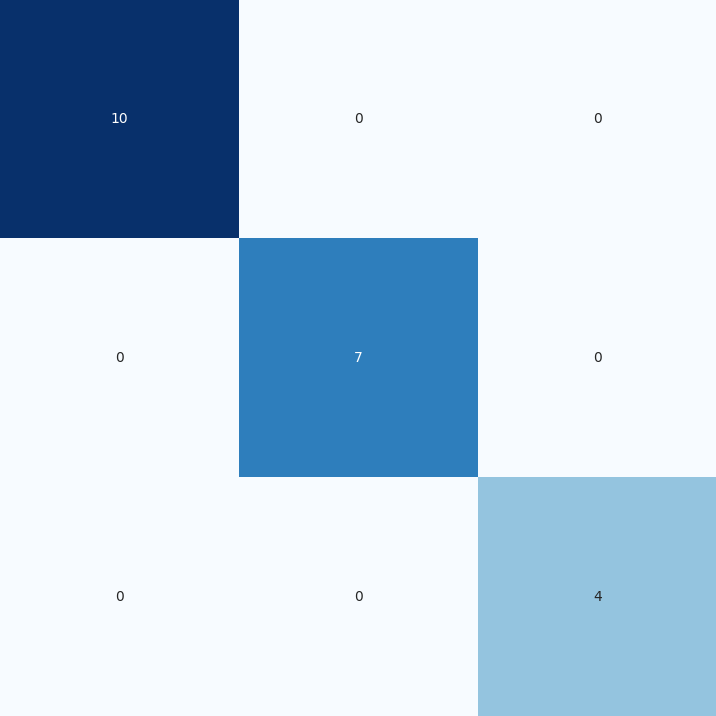
\includegraphics[width=\textwidth]{./class_specific_section/ensemble_plots/ensemble_confusion_matrix_NR_Benefit.png}
        \caption{Ensemble for NR Benefit}
        \label{fig_class:spec_ensemble_nr_benefit}
    \end{minipage}
    \hfill
    \begin{minipage}[b]{0.45\textwidth}
        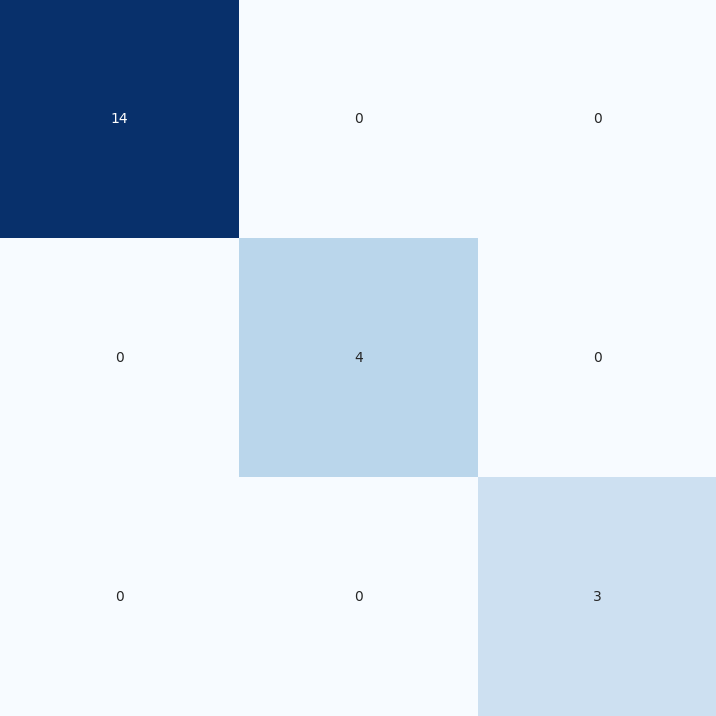
\includegraphics[width=\textwidth]{./class_specific_section/ensemble_plots/ensemble_confusion_matrix_SR_Benefit.png}
        \caption{Ensemble for SR Benefit}
        \label{fig_class:spec_ensemble_sr_benefit}
    \end{minipage}
\end{figure}

\begin{figure}[H]
    \centering
    \begin{minipage}[b]{0.45\textwidth}
        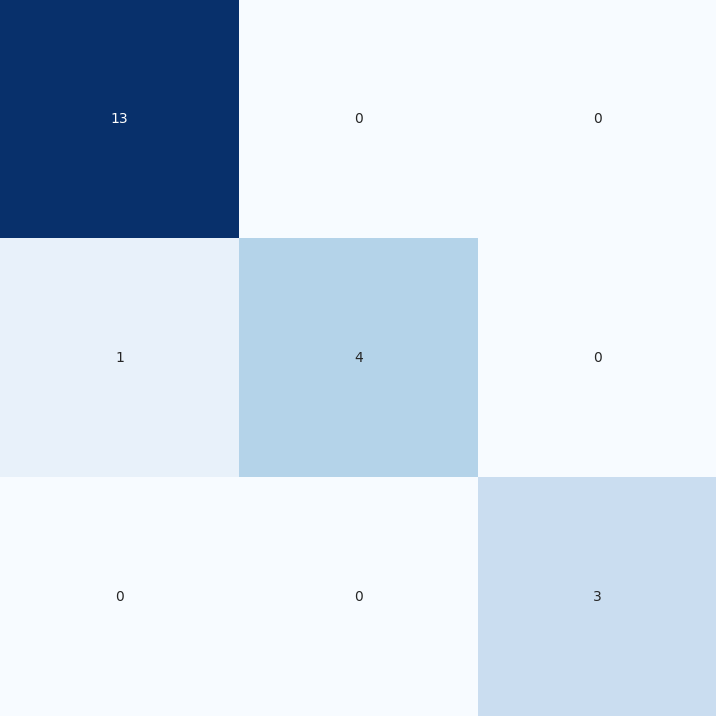
\includegraphics[width=\textwidth]{./class_specific_section/ensemble_plots/ensemble_confusion_matrix_WS_Benefit.png}
        \caption{Ensemble for WS Benefit}
        \label{fig_class:spec_ensemble_ws_benefit}
    \end{minipage}
    \hfill
    \begin{minipage}[b]{0.45\textwidth}
        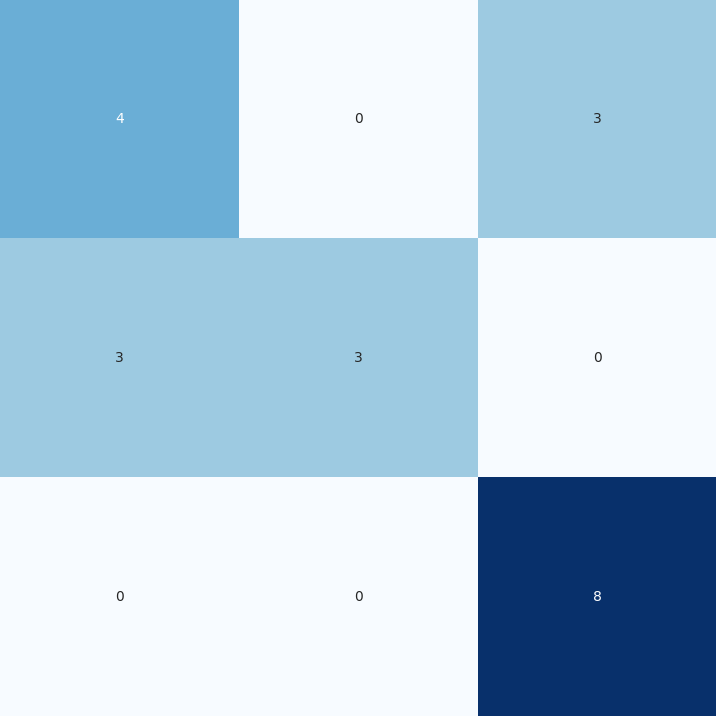
\includegraphics[width=\textwidth]{./class_specific_section/ensemble_plots/ensemble_confusion_matrix_SFST_Benefit.png}
        \caption{Ensemble for SFST Benefit}
        \label{fig_class:spec_ensemble_sfst_benefit}
    \end{minipage}
\end{figure}



\clearpage
\subsection{Regression Models}\label{sec:reg}
\subsubsection{All Features}

\begin{figure}[H]
    \centering
    \begin{minipage}{0.495\textwidth}
        \centering
        \includegraphics[width=\linewidth]{reg_section_all/images_reg_ensemble/ensemble_learning_rmse_plot_top_10_Models_PR.png}
        \caption{PR}
        \label{fig:pr_ensemble}
    \end{minipage}\hfill
    \begin{minipage}{0.495\textwidth}
        \centering
        \includegraphics[width=\linewidth]{reg_section_all/images_reg_ensemble/ensemble_learning_rmse_plot_top_10_Models_NR.png}
        \caption{NR}
        \label{fig:nr_ensemble}
    \end{minipage}
\end{figure}

\begin{figure}[H]
    \centering
    \begin{minipage}{0.495\textwidth}
        \centering
        \includegraphics[width=\linewidth]{reg_section_all/images_reg_ensemble/ensemble_learning_rmse_plot_top_10_Models_SR.png}
        \caption{SR}
        \label{fig:sr_ensemble}
    \end{minipage}\hfill
    \begin{minipage}{0.495\textwidth}
        \centering
        \includegraphics[width=\linewidth]{reg_section_all/images_reg_ensemble/ensemble_learning_rmse_plot_top_10_Models_WS.png}
        \caption{WS}
        \label{fig:ws_ensemble}
    \end{minipage}
\end{figure}

\begin{figure}[H]
    \centering
    \begin{minipage}{0.495\textwidth}
        \centering
        \includegraphics[width=\linewidth]{reg_section_all/images_reg_ensemble/ensemble_learning_rmse_plot_top_10_Models_SFST.png}
        \caption{SFST}
        \label{fig:sfst_ensemble}
    \end{minipage}\hfill
    \begin{minipage}{0.495\textwidth}
        \centering
        \includegraphics[width=\linewidth]{reg_section_all/images_reg_ensemble/ensemble_learning_rmse_plot_top_10_Models_PR_Benefit.png}
        \caption{PR Benefit}
        \label{fig:pr_ben_ensemble}
    \end{minipage}
\end{figure}

\begin{figure}[H]
    \centering
    \begin{minipage}{0.495\textwidth}
        \centering
        \includegraphics[width=\linewidth]{reg_section_all/images_reg_ensemble/ensemble_learning_rmse_plot_top_10_Models_NR_Benefit.png}
        \caption{NR Benefit}
        \label{fig:nr_ben_ensemble}
    \end{minipage}\hfill
    \begin{minipage}{0.495\textwidth}
        \centering
        \includegraphics[width=\linewidth]{reg_section_all/images_reg_ensemble/ensemble_learning_rmse_plot_top_10_Models_SR_Benefit.png}
        \caption{SR Benefit}
        \label{fig:sr_ben_ensemble}
    \end{minipage}
\end{figure}

\begin{figure}[H]
    \centering
    \begin{minipage}{0.495\textwidth}
        \centering
        \includegraphics[width=\linewidth]{reg_section_all/images_reg_ensemble/ensemble_learning_rmse_plot_top_10_Models_WS_Benefit.png}
        \caption{WS Benefit}
        \label{fig:ws_ben_ensemble}
    \end{minipage}\hfill
    \begin{minipage}{0.495\textwidth}
        \centering
        \includegraphics[width=\linewidth]{reg_section_all/images_reg_ensemble/ensemble_learning_rmse_plot_top_10_Models_SFST_Benefit.png}
        \caption{SFST Benefit}
        \label{fig:sfst_ben_ensemble}
    \end{minipage}
\end{figure}
\clearpage
\begin{figure}[H]
    \centering
    \begin{minipage}{0.495\textwidth}
        \centering
        \includegraphics[width=\linewidth]{reg_section_specific/images_reg_training/PR_AdaBoostRegressor_plot.png}
        \caption{PR}
        \label{fig_reg_spec:pr_reg_training}
    \end{minipage}\hfill
    \begin{minipage}{0.495\textwidth}
        \centering
        \includegraphics[width=\linewidth]{reg_section_specific/images_reg_training/NR_AdaBoostRegressor_plot.png}
        \caption{NR}
        \label{fig_reg_spec:nr_reg_training}
    \end{minipage}
\end{figure}

\begin{figure}[H]
    \centering
    \begin{minipage}{0.495\textwidth}
        \centering
        \includegraphics[width=\linewidth]{reg_section_specific/images_reg_training/SR_MLPRegressor_plot.png}
        \caption{SR}
        \label{fig_reg_spec:sr_reg_training}
    \end{minipage}\hfill
    \begin{minipage}{0.495\textwidth}
        \centering
        \includegraphics[width=\linewidth]{reg_section_specific/images_reg_training/WS_MLPRegressor_plot.png}
        \caption{WS}
        \label{fig_reg_spec:ws_reg_training}
    \end{minipage}
\end{figure}

\begin{figure}[H]
    \centering
    \begin{minipage}{0.495\textwidth}
        \centering
        \includegraphics[width=\linewidth]{reg_section_specific/images_reg_training/SFST_AdaBoostRegressor_plot.png}
        \caption{SFST}
        \label{fig_reg_spec:sfst_reg_training}
    \end{minipage}\hfill
    \begin{minipage}{0.495\textwidth}
        \centering
        \includegraphics[width=\linewidth]{reg_section_specific/images_reg_training/PR_Benefit_RandomForestRegressor_plot.png}
        \caption{PR Benefit}
        \label{fig_reg_spec:pr_ben_reg_training}
    \end{minipage}
\end{figure}

\begin{figure}[H]
    \centering
    \begin{minipage}{0.495\textwidth}
        \centering
        \includegraphics[width=\linewidth]{reg_section_specific/images_reg_training/NR_Benefit_MLPRegressor_plot.png}
        \caption{NR Benefit}
        \label{fig_reg_spec:nr_ben_reg_training}
    \end{minipage}\hfill
    \begin{minipage}{0.495\textwidth}
        \centering
        \includegraphics[width=\linewidth]{reg_section_specific/images_reg_training/SR_Benefit_TensorFlow_plot.png}
        \caption{SR Benefit}
        \label{fig_reg_spec:sr_ben_reg_training}
    \end{minipage}
\end{figure}

\begin{figure}[H]
    \centering
    \begin{minipage}{0.495\textwidth}
        \centering
        \includegraphics[width=\linewidth]{reg_section_specific/images_reg_training/WS_Benefit_DecisionTreeRegressor_plot.png}
        \caption{WS Benefit}
        \label{fig_reg_spec:ws_ben_reg_training}
    \end{minipage}\hfill
    \begin{minipage}{0.495\textwidth}
        \centering
        \includegraphics[width=\linewidth]{reg_section_specific/images_reg_training/SFST_Benefit_TheilSenRegressor_plot.png}
        \caption{SFST Benefit}
        \label{fig_reg_spec:sfst_ben_reg_training}
    \end{minipage}
\end{figure}
\clearpage
\begin{enumerate}
    \item \textbf{PCA (Principal Component Analysis)}: A statistical procedure that uses an orthogonal transformation to convert a set of observations of possibly correlated variables into a set of values of linearly uncorrelated variables called principal components.

    \item \textbf{t-SNE (t-Distributed Stochastic Neighbor Embedding)}: A machine learning algorithm for visualization developed by Laurens van der Maaten and Geoffrey Hinton. It is a nonlinear dimensionality reduction technique well-suited for embedding high-dimensional data for visualization in a low-dimensional space of two or three dimensions.

    \item \textbf{UMAP (Uniform Manifold Approximation and Projection)}: A dimension reduction technique that can be used for visualization similarly to t-SNE, but also for general non-linear dimension reduction. It is based on manifold learning techniques and ideas from topological data analysis.

    \item \textbf{Isomap (Isometric Mapping)}: A non-linear dimensionality reduction method based on the geometric distances in the data, which is effective for datasets where nonlinear manifold structures are present.

    \item \textbf{LLE (Locally Linear Embedding)}: Another nonlinear dimension reduction technique that computes low-dimensional, neighborhood-preserving embeddings of high-dimensional inputs.

    \item \textbf{Truncated SVD (Singular Value Decomposition)}: An algorithmic approach for dimensionality reduction that uses truncated singular value decomposition. It is similar to PCA but suitable for sparse datasets.

    \item \textbf{ICA (Independent Component Analysis)}: A computational method for separating a multivariate signal into additive subcomponents that are maximally independent.

    \item \textbf{Kernel PCA}: An extension of PCA using techniques of kernel methods, which uses a kernel function to project dataset into a higher-dimensional space where linear separation is possible.

    \item \textbf{Gaussian Random Projection}: A simple and computationally efficient way to reduce dimensionality by projecting the original data into a randomly generated subspace of lower dimensionality using a Gaussian random matrix.
\end{enumerate}
\clearpage
\begin{figure}[H]
    \centering
    \begin{minipage}{0.45\textwidth}
        \centering
        \includegraphics[width=\linewidth]{reg_section_all/images_dimred_results/dimensionality_reduction_rmse_plot_PR_best.png}
        \caption{PR}
        \label{fig:pr_reg_dimred_training}
    \end{minipage}\hfill
    \begin{minipage}{0.45\textwidth}
        \centering
        \includegraphics[width=\linewidth]{reg_section_all/images_dimred_results/dimensionality_reduction_rmse_plot_NR_best.png}
        \caption{NR}
        \label{fig:nr_reg_dimred_training}
    \end{minipage}
\end{figure}

\begin{figure}[H]
    \centering
    \begin{minipage}{0.45\textwidth}
        \centering
        \includegraphics[width=\linewidth]{reg_section_all/images_dimred_results/dimensionality_reduction_rmse_plot_SR_best.png}
        \caption{SR}
        \label{fig:sr_reg_dimred_training}
    \end{minipage}\hfill
    \begin{minipage}{0.45\textwidth}
        \centering
        \includegraphics[width=\linewidth]{reg_section_all/images_dimred_results/dimensionality_reduction_rmse_plot_WS_best.png}
        \caption{WS}
        \label{fig:ws_reg_dimred_training}
    \end{minipage}
\end{figure}

\begin{figure}[H]
    \centering
    \begin{minipage}{0.45\textwidth}
        \centering
        \includegraphics[width=\linewidth]{reg_section_all/images_dimred_results/dimensionality_reduction_rmse_plot_SFST_best.png}
        \caption{SFST}
        \label{fig:sfst_reg_dimred_training}
    \end{minipage}\hfill
    \begin{minipage}{0.45\textwidth}
        \centering
        \includegraphics[width=\linewidth]{reg_section_all/images_dimred_results/dimensionality_reduction_rmse_plot_PR_Benefit_best.png}
        \caption{PR Benefit}
        \label{fig:pr_ben_reg_dimred_training}
    \end{minipage}
\end{figure}

\begin{figure}[H]
    \centering
    \begin{minipage}{0.45\textwidth}
        \centering
        \includegraphics[width=\linewidth]{reg_section_all/images_dimred_results/dimensionality_reduction_rmse_plot_NR_Benefit_best.png}
        \caption{NR Benefit}
        \label{fig:nr_ben_reg_dimred_training}
    \end{minipage}\hfill
    \begin{minipage}{0.45\textwidth}
        \centering
        \includegraphics[width=\linewidth]{reg_section_all/images_dimred_results/dimensionality_reduction_rmse_plot_SR_Benefit_best.png}
        \caption{SR Benefit}
        \label{fig:sr_ben_reg_dimred_training}
    \end{minipage}
\end{figure}

\begin{figure}[H]
    \centering
    \begin{minipage}{0.45\textwidth}
        \centering
        \includegraphics[width=\linewidth]{reg_section_all/images_dimred_results/dimensionality_reduction_rmse_plot_WS_Benefit_best.png}
        \caption{WS Benefit}
        \label{fig:ws_ben_reg_dimred_training}
    \end{minipage}\hfill
    \begin{minipage}{0.45\textwidth}
        \centering
        \includegraphics[width=\linewidth]{reg_section_all/images_dimred_results/dimensionality_reduction_rmse_plot_SFST_Benefit_best.png}
        \caption{SFST Benefit}
        \label{fig:sfst_ben_reg_dimred_training}
    \end{minipage}
\end{figure}

\clearpage
\begin{longtable}{|p{3cm}|p{2cm}|p{2cm}|p{8cm}|}
\hline
\textbf{Function} & \textbf{RMSE} & \textbf{\# Feat.} & \textbf{Selected Features} \\ \hline
\endfirsthead
\hline
\textbf{Function} & \textbf{RMSE} & \textbf{\# Feat.} & \textbf{Selected Features} \\ \hline
\endhead

WS & 0.4287 & 52 & OF17, OF22, OF24, OF25, OF26, OF28, OF33, F1, F3\_c, F3\_d, F3\_e, F3\_f, F3\_g, F4, F5, F7, F8, F9, F10, F12, F13, F14, F17, F19, F22, F23, F24, F25, F28, F29, F30, F32, F33, F34, F35, F36, F37, F39, F40, F41, F43, F44, F45, F46, F47, F48, F49, F56, F59, F64, F65, S1 \\ \hline
NR & 0.3461 & 79 & OF27, OF18, F5, OF34, F65, S4, S5, OF5, F31, F35, F45, F25, F33, F54, OF13, F24, F34, F3\_g, F43, F2, OF15, F3\_d, OF16, F14, OF9, OF14, F3\_a, F62, F68, OF2, OF11, F7, F3\_f, OF6, F13, F3\_c, F8, OF26, F6, OF38, OF4, F9, OF17, F23, F58, F22, F1, F17, S2, F3\_e, F52, F36, F29, OF28, F40, F4, F30, F28, F47, F44, F15, OF7, F20, OF3, OF25, F51, F21, F3\_b, OF22, F53, F64, F10, OF8, OF10, F56, F50, OF23, F19, F48 \\ \hline
PR & 0.2392 & 71 & OF2, OF6, OF10, OF11, OF16, OF17, OF20, OF21, OF22, OF24, OF25, OF26, OF28, OF30, F1, F3\_a, F3\_b, F3\_c, F3\_d, F3\_e, F3\_f, F3\_g, F4, F5, F6, F7, F8, F9, F10, F12, F13, F14, F15, F16, F17, F18, F19, F20, F22, F23, F24, F25, F28, F29, F30, F32, F33, F34, F35, F36, F37, F38, F39, F40, F41, F43, F44, F45, F46, F47, F49, F50, F51, F52, F53, F56, F63, F64, F65, F67, S1 \\ \hline
SR & 0.5871 & 40 & OF22, OF26, F1, F3\_d, F3\_e, F3\_g, F4, F5, F7, F9, F13, F14, F15, F17, F22, F23, F24, F25, F28, F29, F30, F31, F32, F33, F34, F35, F36, F37, F39, F40, F41, F43, F44, F45, F46, F47, F49, F64, F65, S1 \\ \hline
SFST & 0.4257 & 29 & OF25, OF28, F1, F3\_c, F3\_e, F5, F9, F13, F14, F16, F21, F23, F24, F25, F28, F29, F30, F31, F32, F35, F36, F40, F41, F43, F44, F45, F46, F47, F68 \\ \hline
WS Benefit & 0.9116 & 70 & OF2, OF4, OF5, OF6, OF7, OF14, OF15, OF16, OF17, OF18, OF19, OF21, OF22, OF23, OF24, OF25, OF28, OF31, OF33, OF34, OF37, OF38, F1, F2, F3\_a, F3\_c, F3\_d, F3\_e, F4, F5, F8, F9, F12, F13, F17, F18, F20, F21, F22, F23, F24, F28, F29, F30, F31, F32, F36, F38, F40, F43, F44, F45, F46, F47, F49, F50, F51, F52, F54, F55, F56, F58, F62, F64, F65, F67, F68, S1, S4, S5 \\ \hline
NR Benefit & 1.3035 & 15 & OF5, OF9, OF10, OF15, OF19, OF21, OF23, F1, F3\_c, F14, F31, F41, F43, F46, F47 \\ \hline
PR Benefit & 1.1653 & 7 & OF19, F14, F24, F41, F43, F46, F47 \\ \hline
SR Benefit & 0.7250 & 82 & OF2, OF3, OF4, OF6, OF7, OF8, OF9, OF10, OF11, OF13, OF14, OF16, OF17, OF18, OF19, OF21, OF23, OF24, OF25, OF27, OF28, OF30, OF33, OF34, OF38, F2, F3\_a, F3\_b, F3\_c, F3\_d, F3\_e, F4, F5, F6, F7, F8, F12, F13, F14, F15, F16, F18, F19, F21, F22, F23, F24, F25, F28, F29, F30, F31, F32, F33, F34, F35, F36, F37, F39, F40, F41, F43, F44, F45, F46, F47, F48, F49, F50, F51, F52, F53, F54, F56, F57, F58, F64, F65, F67, F68, S1, S4 \\ \hline
SFST Benefit & 0.6321 & 28 & OF5, OF9, OF18, OF22, OF25, OF28, F1, F2, F3\_e, F3\_g, F5, F9, F13, F14, F20, F23, F24, F25, F28, F29, F30, F31, F41, F43, F44, F45, F46, F47 \\ \hline
\caption{Method with the Lowest RMSE and Number of Features}
\label{tab:lowest_rmse_feat}
\end{longtable}


\begin{longtable}{|p{3cm}|p{2cm}|p{2cm}|p{8cm}|}
\hline
\textbf{Function} & \textbf{RMSE} & \textbf{\# Feat.} & \textbf{Selected Features} \\ \hline
\endfirsthead
\hline
\textbf{Function} & \textbf{RMSE} & \textbf{\# Feat.} & \textbf{Selected Features} \\ \hline
\endhead

WS & 0.8058 & 2 & F31, F43 \\ \hline
NR & 2.4040 & 2 & OF18, S4 \\ \hline
PR & 0.6298 & 2 & F43, F44 \\ \hline
SR & 1.4341 & 2 & F43, F44 \\ \hline
SFST & 0.5892 & 2 & F43, F44 \\ \hline
WS Benefit & 1.5053 & 2 & OF17, OF18 \\ \hline
NR Benefit & 2.2781 & 2 & OF10, OF22 \\ \hline
PR Benefit & 1.3365 & 2 & F41, F44 \\ \hline
SR Benefit & 2.0066 & 2 & OF18, F41 \\ \hline
SFST Benefit & 1.9459 & 2 & OF18, F12 \\ \hline
\caption{Models With Two Features}
\label{tab:lowest_rmse_prop_feat}
\end{longtable}
\clearpage
\begin{figure}[H]
    \centering
    \begin{minipage}{0.45\textwidth}
        \centering
        \includegraphics[width=\linewidth]{reg_section_all/images_reg_featred_graphs/feature_selection_PR.png}
        \caption{PR}
        \label{fig:pr_reg_featred}
    \end{minipage}\hfill
    \begin{minipage}{0.45\textwidth}
        \centering
        \includegraphics[width=\linewidth]{reg_section_all/images_reg_featred_graphs/feature_selection_NR.png}
        \caption{NR}
        \label{fig:nr_reg_featred}
    \end{minipage}
\end{figure}

\begin{figure}[H]
    \centering
    \begin{minipage}{0.45\textwidth}
        \centering
        \includegraphics[width=\linewidth]{reg_section_all/images_reg_featred_graphs/feature_selection_SR.png}
        \caption{SR}
        \label{fig:sr_reg_featred}
    \end{minipage}\hfill
    \begin{minipage}{0.45\textwidth}
        \centering
        \includegraphics[width=\linewidth]{reg_section_all/images_reg_featred_graphs/feature_selection_WS.png}
        \caption{WS}
        \label{fig:ws_reg_featred}
    \end{minipage}
\end{figure}

\begin{figure}[H]
    \centering
    \begin{minipage}{0.45\textwidth}
        \centering
        \includegraphics[width=\linewidth]{reg_section_all/images_reg_featred_graphs/feature_selection_SFST.png}
        \caption{SFST}
        \label{fig:sfst_reg_featred}
    \end{minipage}\hfill
    \begin{minipage}{0.45\textwidth}
        \centering
        \includegraphics[width=\linewidth]{reg_section_all/images_reg_featred_graphs/feature_selection_PR_Benefit.png}
        \caption{PR Benefit}
        \label{fig:pr_ben_reg_featred}
    \end{minipage}
\end{figure}

\begin{figure}[H]
    \centering
    \begin{minipage}{0.45\textwidth}
        \centering
        \includegraphics[width=\linewidth]{reg_section_all/images_reg_featred_graphs/feature_selection_NR_Benefit.png}
        \caption{NR Benefit}
        \label{fig:nr_ben_reg_featred}
    \end{minipage}\hfill
    \begin{minipage}{0.45\textwidth}
        \centering
        \includegraphics[width=\linewidth]{reg_section_all/images_reg_featred_graphs/feature_selection_SR_Benefit.png}
        \caption{SR Benefit}
        \label{fig:sr_ben_reg_featred}
    \end{minipage}
\end{figure}

\begin{figure}[H]
    \centering
    \begin{minipage}{0.45\textwidth}
        \centering
        \includegraphics[width=\linewidth]{reg_section_all/images_reg_featred_graphs/feature_selection_WS_Benefit.png}
        \caption{WS Benefit}
        \label{fig:ws_ben_reg_featred}
    \end{minipage}\hfill
    \begin{minipage}{0.45\textwidth}
        \centering
        \includegraphics[width=\linewidth]{reg_section_all/images_reg_featred_graphs/feature_selection_SFST_Benefit.png}
        \caption{SFST Benefit}
        \label{fig:sfst_ben_reg_featred}
    \end{minipage}
\end{figure}
\clearpage
\begin{figure}[H]
    \centering
    \begin{minipage}{0.45\textwidth}
        \centering
        \includegraphics[width=\linewidth]{reg_section_specxtra/images_reg_featred_ensemble/actual_vs_predicted_best_feature_selection_and_ensemble_PR.png}
        \caption{PR}
        \label{fig_reg_specxtra:pr_reg_featred_best_ensemble}
    \end{minipage}\hfill
    \begin{minipage}{0.45\textwidth}
        \centering
        \includegraphics[width=\linewidth]{reg_section_specxtra/images_reg_featred_ensemble/actual_vs_predicted_best_feature_selection_and_ensemble_NR.png}
        \caption{NR}
        \label{fig_reg_specxtra:nr_reg_featred_best_ensemble}
    \end{minipage}
\end{figure}

\begin{figure}[H]
    \centering
    \begin{minipage}{0.45\textwidth}
        \centering
        \includegraphics[width=\linewidth]{reg_section_specxtra/images_reg_featred_ensemble/actual_vs_predicted_best_feature_selection_and_ensemble_SR.png}
        \caption{SR}
        \label{fig_reg_specxtra:sr_reg_featred_best_ensemble}
    \end{minipage}\hfill
    \begin{minipage}{0.45\textwidth}
        \centering
        \includegraphics[width=\linewidth]{reg_section_specxtra/images_reg_featred_ensemble/actual_vs_predicted_best_feature_selection_and_ensemble_WS.png}
        \caption{WS}
        \label{fig_reg_specxtra:ws_reg_featred_best_ensemble}
    \end{minipage}
\end{figure}

\begin{figure}[H]
    \centering
    \begin{minipage}{0.45\textwidth}
        \centering
        \includegraphics[width=\linewidth]{reg_section_specxtra/images_reg_featred_ensemble/actual_vs_predicted_best_feature_selection_and_ensemble_SFST.png}
        \caption{SFST}
        \label{fig_reg_specxtra:sfst_reg_featred_best_ensemble}
    \end{minipage}\hfill
    \begin{minipage}{0.45\textwidth}
        \centering
        \includegraphics[width=\linewidth]{reg_section_specxtra/images_reg_featred_ensemble/actual_vs_predicted_best_feature_selection_and_ensemble_PR_Benefit.png}
        \caption{PR Benefit}
        \label{fig_reg_specxtra:pr_ben_reg_featred_best_ensemble}
    \end{minipage}
\end{figure}

\begin{figure}[H]
    \centering
    \begin{minipage}{0.45\textwidth}
        \centering
        \includegraphics[width=\linewidth]{reg_section_specxtra/images_reg_featred_ensemble/actual_vs_predicted_best_feature_selection_and_ensemble_NR_Benefit.png}
        \caption{NR Benefit}
        \label{fig_reg_specxtra:nr_ben_reg_featred_best_ensemble}
    \end{minipage}\hfill
    \begin{minipage}{0.45\textwidth}
        \centering
        \includegraphics[width=\linewidth]{reg_section_specxtra/images_reg_featred_ensemble/actual_vs_predicted_best_feature_selection_and_ensemble_SR_Benefit.png}
        \caption{SR Benefit}
        \label{fig_reg_specxtra:sr_ben_reg_featred_best_ensemble}
    \end{minipage}
\end{figure}

\begin{figure}[H]
    \centering
    \begin{minipage}{0.45\textwidth}
        \centering
        \includegraphics[width=\linewidth]{reg_section_specxtra/images_reg_featred_ensemble/actual_vs_predicted_best_feature_selection_and_ensemble_WS_Benefit.png}
        \caption{WS Benefit}
        \label{fig_reg_specxtra:ws_ben_reg_featred_best_ensemble}
    \end{minipage}\hfill
    \begin{minipage}{0.45\textwidth}
        \centering
        \includegraphics[width=\linewidth]{reg_section_specxtra/images_reg_featred_ensemble/actual_vs_predicted_best_feature_selection_and_ensemble_SFST_Benefit.png}
        \caption{SFST Benefit}
        \label{fig_reg_specxtra:sfst_ben_reg_featred_best_ensemble}
    \end{minipage}
\end{figure}

\begin{figure}[H]
    \centering
    \begin{minipage}{0.45\textwidth}
        \centering
        \includegraphics[width=\linewidth]{reg_section_specxtra/images_reg_featred_ensemble/actual_vs_predicted_smallest_feature_selection_and_ensemble_PR.png}
        \caption{PR}
        \label{fig_reg_specxtra:pr_reg_featred_smallest_ensemble}
    \end{minipage}\hfill
    \begin{minipage}{0.45\textwidth}
        \centering
        \includegraphics[width=\linewidth]{reg_section_specxtra/images_reg_featred_ensemble/actual_vs_predicted_smallest_feature_selection_and_ensemble_NR.png}
        \caption{NR}
        \label{fig_reg_specxtra:nr_reg_featred_smallest_ensemble}
    \end{minipage}
\end{figure}

\begin{figure}[H]
    \centering
    \begin{minipage}{0.45\textwidth}
        \centering
        \includegraphics[width=\linewidth]{reg_section_specxtra/images_reg_featred_ensemble/actual_vs_predicted_smallest_feature_selection_and_ensemble_SR.png}
        \caption{SR}
        \label{fig_reg_specxtra:sr_reg_featred_smallest_ensemble}
    \end{minipage}\hfill
    \begin{minipage}{0.45\textwidth}
        \centering
        \includegraphics[width=\linewidth]{reg_section_specxtra/images_reg_featred_ensemble/actual_vs_predicted_smallest_feature_selection_and_ensemble_WS.png}
        \caption{WS}
        \label{fig_reg_specxtra:ws_reg_featred_smallest_ensemble}
    \end{minipage}
\end{figure}

\begin{figure}[H]
    \centering
    \begin{minipage}{0.45\textwidth}
        \centering
        \includegraphics[width=\linewidth]{reg_section_specxtra/images_reg_featred_ensemble/actual_vs_predicted_smallest_feature_selection_and_ensemble_SFST.png}
        \caption{SFST}
        \label{fig_reg_specxtra:sfst_reg_featred_smallest_ensemble}
    \end{minipage}\hfill
    \begin{minipage}{0.45\textwidth}
        \centering
        \includegraphics[width=\linewidth]{reg_section_specxtra/images_reg_featred_ensemble/actual_vs_predicted_smallest_feature_selection_and_ensemble_PR_Benefit.png}
        \caption{PR Benefit}
        \label{fig_reg_specxtra:pr_ben_reg_featred_smallest_ensemble}
    \end{minipage}
\end{figure}

\begin{figure}[H]
    \centering
    \begin{minipage}{0.45\textwidth}
        \centering
        \includegraphics[width=\linewidth]{reg_section_specxtra/images_reg_featred_ensemble/actual_vs_predicted_smallest_feature_selection_and_ensemble_NR_Benefit.png}
        \caption{NR Benefit}
        \label{fig_reg_specxtra:nr_ben_reg_featred_smallest_ensemble}
    \end{minipage}\hfill
    \begin{minipage}{0.45\textwidth}
        \centering
        \includegraphics[width=\linewidth]{reg_section_specxtra/images_reg_featred_ensemble/actual_vs_predicted_smallest_feature_selection_and_ensemble_SR_Benefit.png}
        \caption{SR Benefit}
        \label{fig_reg_specxtra:sr_ben_reg_featred_smallest_ensemble}
    \end{minipage}
\end{figure}

\begin{figure}[H]
    \centering
    \begin{minipage}{0.45\textwidth}
        \centering
        \includegraphics[width=\linewidth]{reg_section_specxtra/images_reg_featred_ensemble/actual_vs_predicted_smallest_feature_selection_and_ensemble_WS_Benefit.png}
        \caption{WS Benefit}
        \label{fig_reg_specxtra:ws_ben_reg_featred_smallest_ensemble}
    \end{minipage}\hfill
    \begin{minipage}{0.45\textwidth}
        \centering
        \includegraphics[width=\linewidth]{reg_section_specxtra/images_reg_featred_ensemble/actual_vs_predicted_smallest_feature_selection_and_ensemble_SFST_Benefit.png}
        \caption{SFST Benefit}
        \label{fig_reg_specxtra:sfst_ben_reg_featred_smallest_ensemble}
    \end{minipage}
\end{figure}
\clearpage
\begin{longtable}{|p{3cm}|p{2cm}|p{2cm}|}
\hline
\textbf{Function} & \textbf{RMSE} & \textbf{\# Feat.} \\ \hline

WS & 0.4285 & 57  \\ \hline
NR & 0.3347 & 103  \\ \hline
PR &  0.2470 & 78 \\ \hline
SR &  0.5908 & 41  \\ \hline
SFST &  0.4289 & 39  \\ \hline
WS Benefit & 0.9033 & 103  \\ \hline
NR Benefit &  1.1703 & 72 \\ \hline
PR Benefit &  0.9819 & 23  \\ \hline
SR Benefit &  0.6934 & 103  \\ \hline
SFST Benefit & 0.6477  & 93   \\ \hline
\caption{Ensemble Learning using All Features}
\label{fig_mse_spec:lowest_best_rmse_featred}
\end{longtable}

\begin{longtable}{|p{3cm}|p{2cm}|p{2cm}|p{8cm}|}
\hline
\textbf{Function} & \textbf{RMSE} & \textbf{\# Feat.} & \textbf{Selected Features} \\ \hline

WS & 0.7547 & 6 & F22,F24,F31,F43,F44,F46 \\ \hline
NR & 0.6878 & 20 & F1,F12,F23,F24,F25,F28,F29,F31,F43,F44, F45,D46,D65,F68,OF18,OF34,OF37,S2,S4,S5 \\ \hline
PR &  0.7463 & 4 &F43,F44,F45,F46 \\ \hline
SR &  1.1949 & 8 & F1,F24,F28,F31,F43,F44,F45,F46\\ \hline
SFST &  0.5659 & 4 & F43,F44,F45,F46\\ \hline
WS Benefit & 1.0354 & 6 & F51,OF15,OF17,OF18,OF23,OF24 \\ \hline
NR Benefit &  1.9944 & 7 &  F20,F31,F3c,F41,F43,OF18,0F22 \\ \hline
PR Benefit &  1.2953 & 6 &  F14,F3c,F41,F43,F44.OF19\\ \hline
SR Benefit &  1.2354 & 8 &  F12,F43,F44,F45,F46,F53,OF18,OF30 \\ \hline
SFST Benefit & 1.1440  & 20 & F1, F12, F14, F23, F25, F29, F31,  F39, F3d, F43, F44, F45, F46,  F53, F57, F6, OF14, OF18, OF28, OF30 \\ \hline
\caption{Ensemble Learning using limited features}
\label{fig_mse_spec:lowest_smallest_rmse_featred}
\end{longtable}
\clearpage
\begin{longtable}{|p{2cm}|p{2cm}|p{2cm}|p{2cm}|p{2cm}|p{4cm}|}
\hline
\textbf{Model} & \textbf{Lower Acc.} & \textbf{Moderate Acc.} & \textbf{Higher Acc.} & \textbf{Overall Acc.} & \textbf{Top Features} \\ \hline
\endfirsthead
\hline
\textbf{Model} & \textbf{Lower Acc.} & \textbf{Moderate Acc.} & \textbf{Higher Acc.} & \textbf{Overall Acc.} & \textbf{Top Features} \\ \hline
\endhead

WS & 80.81\% & 64.20\% & 70.37\% & 74.07\% & Provincial\_Class, Hydrogeomorphic\_Class, OF22, F22, F28, F31, F43, F44, F45 \\ \hline
PR & 13.89\% & 77.78\% & 87.50\% & 69.31\% & Provincial\_Class, Federal\_Class, F43, F44, F45 \\ \hline
NR & 32.80\% & 65.08\% & 76.19\% & 58.02\% & Provincial\_Class, F24, F43, F44, F45 \\ \hline
SR & 62.22\% & 60.00\% & 62.35\% & 61.73\% & F28, F29, F31, F44, F45 \\ \hline
SFST & 56.17\% & 60.85\% & 76.39\% & 65.43\% & F1, F43 \\ \hline
WS Benefit & 68.35\% & 46.56\% & 44.44\% & 57.67\% & Hydrogeomorphic\_Class, OF17, OF18, OF23, OF24, F51 \\ \hline
PR Benefit & 80.00\% & 44.97\% & 29.63\% & 58.73\% & Regime, Moss\_Cover, Living\_Moss\_Depth, OF19, OF20, OF21, OF22, OF24, F41 \\ \hline
NR Benefit & 70.74\% & 80.42\% & 49.07\% & 69.84\% & Living\_Moss\_Depth, OF9, OF10, OF19, OF20, OF21, OF22, OF23, F41 \\ \hline
SR Benefit & 93.70\% & 53.91\% & 0.00\% & 67.72\% & Provincial\_Class, Federal\_Class, Regime, Vegetation\_Type, Living\_Moss\_Depth, Organic\_Depth, Hydrogeomorphic\_Class, OF18, OF24, F41 \\ \hline
SFST Benefit & 59.72\% & 32.10\% & 48.15\% & 47.97\% & Provincial\_Class, Federal\_Class, Moss\_Cover, Surface\_Water\_Present, Hydrogeomorphic\_Class, OF18, OF22, OF25, OF28 \\ \hline
\caption{Classification Accuracies and Top Features for Various Models}
\label{tab:grouping_1d}
\end{longtable}

\begin{longtable}{|p{1.5cm}|p{2.0cm}|p{2.0cm}|p{2.0cm}|p{2.0cm}|p{4cm}|}
\hline
\textbf{Model} & \textbf{Lower Acc.} & \textbf{Moderate Acc.} & \textbf{Higher Acc.} & \textbf{Overall Acc.} & \textbf{Top Features} \\ \hline
\endfirsthead
\hline
\textbf{Model} & \textbf{Lower Acc.} & \textbf{Moderate Acc.} & \textbf{Higher Acc.} & \textbf{Overall Acc.} & \textbf{Top Features} \\ \hline
\endhead

WS & 100.00\% & 50.00\% & 100.00\% & 85.71\% & F22, F31, F43, F44, F46, F5, OF18, OF27 \\ \hline
PR & 0.00\% & 100.00\% & 100.00\% & 76.19\% & F43, F44, F45, F5, OF18, OF27 \\ \hline
NR & 0.00\% & 71.43\% & 42.86\% & 80.95\% & F43, F44, F45, F5, OF18, OF27, OF34, S4 \\ \hline
SR & 30.00\% & 80.00\% & 50.00\% & 90.48\% & F24, F28, F31, F43, F44, F45, F5, OF18, OF27 \\ \hline
SFST & 100.00\% & 42.86\% & 100.00\% & 80.95\% & F43, F44, F45, F46, OF18, OF27 \\ \hline
WS Benefit & 54.55\% & 71.43\% & 66.67\% & 90.48\% & F5, OF17, OF18, OF23, OF27, OF34, S4 \\ \hline
PR Benefit & 100.00\% & 85.71\% & 25.00\% & 80.95\% & F14, F3\_c, F41, F44, OF18, OF19, OF27 \\ \hline
NR Benefit & 100.00\% & 85.71\% & 50.00\% & 85.71\% & F41, F5, OF10, OF18, OF19, OF22, OF27, OF9 \\ \hline
SR Benefit & 100.00\% & 0.00\% & 0.00\% & 85.71\% & F12, F41, OF18, OF22, OF27, OF30 \\ \hline
SFST Benefit & 37.50\% & 100.00\% & 42.86\% & 80.95\% & F12, F43, F44, F45, F5, OF18, OF27, OF30 \\ \hline
\caption{Ensemble Model Accuracies}
\label{tab:grouping_2d}
\end{longtable}

\begin{longtable}{|p{1.5cm}|p{2.0cm}|p{2.0cm}|p{2.0cm}|p{2.0cm}|p{4cm}|}
\hline
\textbf{Model} & \textbf{Lower Acc.} & \textbf{Moderate Acc.} & \textbf{Higher Acc.} & \textbf{Overall Acc.} & \textbf{Top Features} \\ \hline
\endfirsthead
\hline
\textbf{Model} & \textbf{Lower Acc.} & \textbf{Moderate Acc.} & \textbf{Higher Acc.} & \textbf{Overall Acc.} & \textbf{Top Features} \\ \hline
\endhead

WS & 100.00\% & 50.00\% & 75.00\% & 85.71\% & F22, F31, F43, F44, F46, F5, OF18, OF27 \\ \hline
PR & 0.00\% & 100.00\% & 100.00\% & 76.19\% & F43, F44, F45, F5, OF18, OF27 \\ \hline
NR & 0.00\% & 85.71\% & 42.86\% & 61.90\% & F43, F44, F45, F5, OF18, OF27, OF34, S4 \\ \hline
SR & 30.00\% & 80.00\% & 33.33\% & 85.71\% & F24, F28, F31, F43, F44, F45, F5, OF18, OF27 \\ \hline
SFST & 100.00\% & 42.86\% & 100.00\% & 80.95\% & F43, F44, F45, F46, OF18, OF27 \\ \hline
WS Benefit & 36.36\% & 71.43\% & 66.67\% & 80.95\% & F5, OF17, OF18, OF23, OF27, OF34, S4 \\ \hline
PR Benefit & 100.00\% & 85.71\% & 25.00\% & 80.95\% & F14, F3\_c, F41, F44, OF18, OF19, OF27 \\ \hline
NR Benefit & 100.00\% & 85.71\% & 50.00\% & 76.19\% & F41, F5, OF10, OF18, OF19, OF22, OF27, OF9 \\ \hline
SR Benefit & 100.00\% & 0.00\% & 0.00\% & 47.62\% & F12, F41, OF18, OF22, OF27, OF30 \\ \hline
SFST Benefit & 37.50\% & 100.00\% & 42.86\% & 57.14\% & F12, F43, F44, F45, F5, OF18, OF27, OF30 \\ \hline

\caption{Voting System Accuracies}
\label{tab:grouping_3d}
\end{longtable}

\clearpage

\subsubsection{Specific Features}
\begin{figure}[H]
    \centering
    \begin{minipage}{0.495\textwidth}
        \centering
        \includegraphics[width=\linewidth]{reg_section_specific/images_reg_training/PR_AdaBoostRegressor_plot.png}
        \caption{PR}
        \label{fig_reg_spec:pr_reg_training}
    \end{minipage}\hfill
    \begin{minipage}{0.495\textwidth}
        \centering
        \includegraphics[width=\linewidth]{reg_section_specific/images_reg_training/NR_AdaBoostRegressor_plot.png}
        \caption{NR}
        \label{fig_reg_spec:nr_reg_training}
    \end{minipage}
\end{figure}

\begin{figure}[H]
    \centering
    \begin{minipage}{0.495\textwidth}
        \centering
        \includegraphics[width=\linewidth]{reg_section_specific/images_reg_training/SR_MLPRegressor_plot.png}
        \caption{SR}
        \label{fig_reg_spec:sr_reg_training}
    \end{minipage}\hfill
    \begin{minipage}{0.495\textwidth}
        \centering
        \includegraphics[width=\linewidth]{reg_section_specific/images_reg_training/WS_MLPRegressor_plot.png}
        \caption{WS}
        \label{fig_reg_spec:ws_reg_training}
    \end{minipage}
\end{figure}

\begin{figure}[H]
    \centering
    \begin{minipage}{0.495\textwidth}
        \centering
        \includegraphics[width=\linewidth]{reg_section_specific/images_reg_training/SFST_AdaBoostRegressor_plot.png}
        \caption{SFST}
        \label{fig_reg_spec:sfst_reg_training}
    \end{minipage}\hfill
    \begin{minipage}{0.495\textwidth}
        \centering
        \includegraphics[width=\linewidth]{reg_section_specific/images_reg_training/PR_Benefit_RandomForestRegressor_plot.png}
        \caption{PR Benefit}
        \label{fig_reg_spec:pr_ben_reg_training}
    \end{minipage}
\end{figure}

\begin{figure}[H]
    \centering
    \begin{minipage}{0.495\textwidth}
        \centering
        \includegraphics[width=\linewidth]{reg_section_specific/images_reg_training/NR_Benefit_MLPRegressor_plot.png}
        \caption{NR Benefit}
        \label{fig_reg_spec:nr_ben_reg_training}
    \end{minipage}\hfill
    \begin{minipage}{0.495\textwidth}
        \centering
        \includegraphics[width=\linewidth]{reg_section_specific/images_reg_training/SR_Benefit_TensorFlow_plot.png}
        \caption{SR Benefit}
        \label{fig_reg_spec:sr_ben_reg_training}
    \end{minipage}
\end{figure}

\begin{figure}[H]
    \centering
    \begin{minipage}{0.495\textwidth}
        \centering
        \includegraphics[width=\linewidth]{reg_section_specific/images_reg_training/WS_Benefit_DecisionTreeRegressor_plot.png}
        \caption{WS Benefit}
        \label{fig_reg_spec:ws_ben_reg_training}
    \end{minipage}\hfill
    \begin{minipage}{0.495\textwidth}
        \centering
        \includegraphics[width=\linewidth]{reg_section_specific/images_reg_training/SFST_Benefit_TheilSenRegressor_plot.png}
        \caption{SFST Benefit}
        \label{fig_reg_spec:sfst_ben_reg_training}
    \end{minipage}
\end{figure}
\clearpage
\begin{figure}[H]
    \centering
    \begin{minipage}{0.495\textwidth}
        \centering
        \includegraphics[width=\linewidth]{reg_section_all/images_reg_ensemble/ensemble_learning_rmse_plot_top_10_Models_PR.png}
        \caption{PR}
        \label{fig:pr_ensemble}
    \end{minipage}\hfill
    \begin{minipage}{0.495\textwidth}
        \centering
        \includegraphics[width=\linewidth]{reg_section_all/images_reg_ensemble/ensemble_learning_rmse_plot_top_10_Models_NR.png}
        \caption{NR}
        \label{fig:nr_ensemble}
    \end{minipage}
\end{figure}

\begin{figure}[H]
    \centering
    \begin{minipage}{0.495\textwidth}
        \centering
        \includegraphics[width=\linewidth]{reg_section_all/images_reg_ensemble/ensemble_learning_rmse_plot_top_10_Models_SR.png}
        \caption{SR}
        \label{fig:sr_ensemble}
    \end{minipage}\hfill
    \begin{minipage}{0.495\textwidth}
        \centering
        \includegraphics[width=\linewidth]{reg_section_all/images_reg_ensemble/ensemble_learning_rmse_plot_top_10_Models_WS.png}
        \caption{WS}
        \label{fig:ws_ensemble}
    \end{minipage}
\end{figure}

\begin{figure}[H]
    \centering
    \begin{minipage}{0.495\textwidth}
        \centering
        \includegraphics[width=\linewidth]{reg_section_all/images_reg_ensemble/ensemble_learning_rmse_plot_top_10_Models_SFST.png}
        \caption{SFST}
        \label{fig:sfst_ensemble}
    \end{minipage}\hfill
    \begin{minipage}{0.495\textwidth}
        \centering
        \includegraphics[width=\linewidth]{reg_section_all/images_reg_ensemble/ensemble_learning_rmse_plot_top_10_Models_PR_Benefit.png}
        \caption{PR Benefit}
        \label{fig:pr_ben_ensemble}
    \end{minipage}
\end{figure}

\begin{figure}[H]
    \centering
    \begin{minipage}{0.495\textwidth}
        \centering
        \includegraphics[width=\linewidth]{reg_section_all/images_reg_ensemble/ensemble_learning_rmse_plot_top_10_Models_NR_Benefit.png}
        \caption{NR Benefit}
        \label{fig:nr_ben_ensemble}
    \end{minipage}\hfill
    \begin{minipage}{0.495\textwidth}
        \centering
        \includegraphics[width=\linewidth]{reg_section_all/images_reg_ensemble/ensemble_learning_rmse_plot_top_10_Models_SR_Benefit.png}
        \caption{SR Benefit}
        \label{fig:sr_ben_ensemble}
    \end{minipage}
\end{figure}

\begin{figure}[H]
    \centering
    \begin{minipage}{0.495\textwidth}
        \centering
        \includegraphics[width=\linewidth]{reg_section_all/images_reg_ensemble/ensemble_learning_rmse_plot_top_10_Models_WS_Benefit.png}
        \caption{WS Benefit}
        \label{fig:ws_ben_ensemble}
    \end{minipage}\hfill
    \begin{minipage}{0.495\textwidth}
        \centering
        \includegraphics[width=\linewidth]{reg_section_all/images_reg_ensemble/ensemble_learning_rmse_plot_top_10_Models_SFST_Benefit.png}
        \caption{SFST Benefit}
        \label{fig:sfst_ben_ensemble}
    \end{minipage}
\end{figure}
\clearpage
\begin{longtable}{|p{3cm}|p{2cm}|p{2cm}|p{8cm}|}
\hline
\textbf{Function} & \textbf{RMSE} & \textbf{\# Feat.} & \textbf{Selected Features} \\ \hline
\endfirsthead
\hline
\textbf{Function} & \textbf{RMSE} & \textbf{\# Feat.} & \textbf{Selected Features} \\ \hline
\endhead

WS & 0.4287 & 52 & OF17, OF22, OF24, OF25, OF26, OF28, OF33, F1, F3\_c, F3\_d, F3\_e, F3\_f, F3\_g, F4, F5, F7, F8, F9, F10, F12, F13, F14, F17, F19, F22, F23, F24, F25, F28, F29, F30, F32, F33, F34, F35, F36, F37, F39, F40, F41, F43, F44, F45, F46, F47, F48, F49, F56, F59, F64, F65, S1 \\ \hline
NR & 0.3461 & 79 & OF27, OF18, F5, OF34, F65, S4, S5, OF5, F31, F35, F45, F25, F33, F54, OF13, F24, F34, F3\_g, F43, F2, OF15, F3\_d, OF16, F14, OF9, OF14, F3\_a, F62, F68, OF2, OF11, F7, F3\_f, OF6, F13, F3\_c, F8, OF26, F6, OF38, OF4, F9, OF17, F23, F58, F22, F1, F17, S2, F3\_e, F52, F36, F29, OF28, F40, F4, F30, F28, F47, F44, F15, OF7, F20, OF3, OF25, F51, F21, F3\_b, OF22, F53, F64, F10, OF8, OF10, F56, F50, OF23, F19, F48 \\ \hline
PR & 0.2392 & 71 & OF2, OF6, OF10, OF11, OF16, OF17, OF20, OF21, OF22, OF24, OF25, OF26, OF28, OF30, F1, F3\_a, F3\_b, F3\_c, F3\_d, F3\_e, F3\_f, F3\_g, F4, F5, F6, F7, F8, F9, F10, F12, F13, F14, F15, F16, F17, F18, F19, F20, F22, F23, F24, F25, F28, F29, F30, F32, F33, F34, F35, F36, F37, F38, F39, F40, F41, F43, F44, F45, F46, F47, F49, F50, F51, F52, F53, F56, F63, F64, F65, F67, S1 \\ \hline
SR & 0.5871 & 40 & OF22, OF26, F1, F3\_d, F3\_e, F3\_g, F4, F5, F7, F9, F13, F14, F15, F17, F22, F23, F24, F25, F28, F29, F30, F31, F32, F33, F34, F35, F36, F37, F39, F40, F41, F43, F44, F45, F46, F47, F49, F64, F65, S1 \\ \hline
SFST & 0.4257 & 29 & OF25, OF28, F1, F3\_c, F3\_e, F5, F9, F13, F14, F16, F21, F23, F24, F25, F28, F29, F30, F31, F32, F35, F36, F40, F41, F43, F44, F45, F46, F47, F68 \\ \hline
WS Benefit & 0.9116 & 70 & OF2, OF4, OF5, OF6, OF7, OF14, OF15, OF16, OF17, OF18, OF19, OF21, OF22, OF23, OF24, OF25, OF28, OF31, OF33, OF34, OF37, OF38, F1, F2, F3\_a, F3\_c, F3\_d, F3\_e, F4, F5, F8, F9, F12, F13, F17, F18, F20, F21, F22, F23, F24, F28, F29, F30, F31, F32, F36, F38, F40, F43, F44, F45, F46, F47, F49, F50, F51, F52, F54, F55, F56, F58, F62, F64, F65, F67, F68, S1, S4, S5 \\ \hline
NR Benefit & 1.3035 & 15 & OF5, OF9, OF10, OF15, OF19, OF21, OF23, F1, F3\_c, F14, F31, F41, F43, F46, F47 \\ \hline
PR Benefit & 1.1653 & 7 & OF19, F14, F24, F41, F43, F46, F47 \\ \hline
SR Benefit & 0.7250 & 82 & OF2, OF3, OF4, OF6, OF7, OF8, OF9, OF10, OF11, OF13, OF14, OF16, OF17, OF18, OF19, OF21, OF23, OF24, OF25, OF27, OF28, OF30, OF33, OF34, OF38, F2, F3\_a, F3\_b, F3\_c, F3\_d, F3\_e, F4, F5, F6, F7, F8, F12, F13, F14, F15, F16, F18, F19, F21, F22, F23, F24, F25, F28, F29, F30, F31, F32, F33, F34, F35, F36, F37, F39, F40, F41, F43, F44, F45, F46, F47, F48, F49, F50, F51, F52, F53, F54, F56, F57, F58, F64, F65, F67, F68, S1, S4 \\ \hline
SFST Benefit & 0.6321 & 28 & OF5, OF9, OF18, OF22, OF25, OF28, F1, F2, F3\_e, F3\_g, F5, F9, F13, F14, F20, F23, F24, F25, F28, F29, F30, F31, F41, F43, F44, F45, F46, F47 \\ \hline
\caption{Method with the Lowest RMSE and Number of Features}
\label{tab:lowest_rmse_feat}
\end{longtable}


\begin{longtable}{|p{3cm}|p{2cm}|p{2cm}|p{8cm}|}
\hline
\textbf{Function} & \textbf{RMSE} & \textbf{\# Feat.} & \textbf{Selected Features} \\ \hline
\endfirsthead
\hline
\textbf{Function} & \textbf{RMSE} & \textbf{\# Feat.} & \textbf{Selected Features} \\ \hline
\endhead

WS & 0.8058 & 2 & F31, F43 \\ \hline
NR & 2.4040 & 2 & OF18, S4 \\ \hline
PR & 0.6298 & 2 & F43, F44 \\ \hline
SR & 1.4341 & 2 & F43, F44 \\ \hline
SFST & 0.5892 & 2 & F43, F44 \\ \hline
WS Benefit & 1.5053 & 2 & OF17, OF18 \\ \hline
NR Benefit & 2.2781 & 2 & OF10, OF22 \\ \hline
PR Benefit & 1.3365 & 2 & F41, F44 \\ \hline
SR Benefit & 2.0066 & 2 & OF18, F41 \\ \hline
SFST Benefit & 1.9459 & 2 & OF18, F12 \\ \hline
\caption{Models With Two Features}
\label{tab:lowest_rmse_prop_feat}
\end{longtable}
\begin{figure}[H]
    \centering
    \begin{minipage}{0.45\textwidth}
        \centering
        \includegraphics[width=\linewidth]{reg_section_specxtra/images_reg_featred_ensemble/actual_vs_predicted_best_feature_selection_and_ensemble_PR.png}
        \caption{PR}
        \label{fig_reg_specxtra:pr_reg_featred_best_ensemble}
    \end{minipage}\hfill
    \begin{minipage}{0.45\textwidth}
        \centering
        \includegraphics[width=\linewidth]{reg_section_specxtra/images_reg_featred_ensemble/actual_vs_predicted_best_feature_selection_and_ensemble_NR.png}
        \caption{NR}
        \label{fig_reg_specxtra:nr_reg_featred_best_ensemble}
    \end{minipage}
\end{figure}

\begin{figure}[H]
    \centering
    \begin{minipage}{0.45\textwidth}
        \centering
        \includegraphics[width=\linewidth]{reg_section_specxtra/images_reg_featred_ensemble/actual_vs_predicted_best_feature_selection_and_ensemble_SR.png}
        \caption{SR}
        \label{fig_reg_specxtra:sr_reg_featred_best_ensemble}
    \end{minipage}\hfill
    \begin{minipage}{0.45\textwidth}
        \centering
        \includegraphics[width=\linewidth]{reg_section_specxtra/images_reg_featred_ensemble/actual_vs_predicted_best_feature_selection_and_ensemble_WS.png}
        \caption{WS}
        \label{fig_reg_specxtra:ws_reg_featred_best_ensemble}
    \end{minipage}
\end{figure}

\begin{figure}[H]
    \centering
    \begin{minipage}{0.45\textwidth}
        \centering
        \includegraphics[width=\linewidth]{reg_section_specxtra/images_reg_featred_ensemble/actual_vs_predicted_best_feature_selection_and_ensemble_SFST.png}
        \caption{SFST}
        \label{fig_reg_specxtra:sfst_reg_featred_best_ensemble}
    \end{minipage}\hfill
    \begin{minipage}{0.45\textwidth}
        \centering
        \includegraphics[width=\linewidth]{reg_section_specxtra/images_reg_featred_ensemble/actual_vs_predicted_best_feature_selection_and_ensemble_PR_Benefit.png}
        \caption{PR Benefit}
        \label{fig_reg_specxtra:pr_ben_reg_featred_best_ensemble}
    \end{minipage}
\end{figure}

\begin{figure}[H]
    \centering
    \begin{minipage}{0.45\textwidth}
        \centering
        \includegraphics[width=\linewidth]{reg_section_specxtra/images_reg_featred_ensemble/actual_vs_predicted_best_feature_selection_and_ensemble_NR_Benefit.png}
        \caption{NR Benefit}
        \label{fig_reg_specxtra:nr_ben_reg_featred_best_ensemble}
    \end{minipage}\hfill
    \begin{minipage}{0.45\textwidth}
        \centering
        \includegraphics[width=\linewidth]{reg_section_specxtra/images_reg_featred_ensemble/actual_vs_predicted_best_feature_selection_and_ensemble_SR_Benefit.png}
        \caption{SR Benefit}
        \label{fig_reg_specxtra:sr_ben_reg_featred_best_ensemble}
    \end{minipage}
\end{figure}

\begin{figure}[H]
    \centering
    \begin{minipage}{0.45\textwidth}
        \centering
        \includegraphics[width=\linewidth]{reg_section_specxtra/images_reg_featred_ensemble/actual_vs_predicted_best_feature_selection_and_ensemble_WS_Benefit.png}
        \caption{WS Benefit}
        \label{fig_reg_specxtra:ws_ben_reg_featred_best_ensemble}
    \end{minipage}\hfill
    \begin{minipage}{0.45\textwidth}
        \centering
        \includegraphics[width=\linewidth]{reg_section_specxtra/images_reg_featred_ensemble/actual_vs_predicted_best_feature_selection_and_ensemble_SFST_Benefit.png}
        \caption{SFST Benefit}
        \label{fig_reg_specxtra:sfst_ben_reg_featred_best_ensemble}
    \end{minipage}
\end{figure}

\begin{figure}[H]
    \centering
    \begin{minipage}{0.45\textwidth}
        \centering
        \includegraphics[width=\linewidth]{reg_section_specxtra/images_reg_featred_ensemble/actual_vs_predicted_smallest_feature_selection_and_ensemble_PR.png}
        \caption{PR}
        \label{fig_reg_specxtra:pr_reg_featred_smallest_ensemble}
    \end{minipage}\hfill
    \begin{minipage}{0.45\textwidth}
        \centering
        \includegraphics[width=\linewidth]{reg_section_specxtra/images_reg_featred_ensemble/actual_vs_predicted_smallest_feature_selection_and_ensemble_NR.png}
        \caption{NR}
        \label{fig_reg_specxtra:nr_reg_featred_smallest_ensemble}
    \end{minipage}
\end{figure}

\begin{figure}[H]
    \centering
    \begin{minipage}{0.45\textwidth}
        \centering
        \includegraphics[width=\linewidth]{reg_section_specxtra/images_reg_featred_ensemble/actual_vs_predicted_smallest_feature_selection_and_ensemble_SR.png}
        \caption{SR}
        \label{fig_reg_specxtra:sr_reg_featred_smallest_ensemble}
    \end{minipage}\hfill
    \begin{minipage}{0.45\textwidth}
        \centering
        \includegraphics[width=\linewidth]{reg_section_specxtra/images_reg_featred_ensemble/actual_vs_predicted_smallest_feature_selection_and_ensemble_WS.png}
        \caption{WS}
        \label{fig_reg_specxtra:ws_reg_featred_smallest_ensemble}
    \end{minipage}
\end{figure}

\begin{figure}[H]
    \centering
    \begin{minipage}{0.45\textwidth}
        \centering
        \includegraphics[width=\linewidth]{reg_section_specxtra/images_reg_featred_ensemble/actual_vs_predicted_smallest_feature_selection_and_ensemble_SFST.png}
        \caption{SFST}
        \label{fig_reg_specxtra:sfst_reg_featred_smallest_ensemble}
    \end{minipage}\hfill
    \begin{minipage}{0.45\textwidth}
        \centering
        \includegraphics[width=\linewidth]{reg_section_specxtra/images_reg_featred_ensemble/actual_vs_predicted_smallest_feature_selection_and_ensemble_PR_Benefit.png}
        \caption{PR Benefit}
        \label{fig_reg_specxtra:pr_ben_reg_featred_smallest_ensemble}
    \end{minipage}
\end{figure}

\begin{figure}[H]
    \centering
    \begin{minipage}{0.45\textwidth}
        \centering
        \includegraphics[width=\linewidth]{reg_section_specxtra/images_reg_featred_ensemble/actual_vs_predicted_smallest_feature_selection_and_ensemble_NR_Benefit.png}
        \caption{NR Benefit}
        \label{fig_reg_specxtra:nr_ben_reg_featred_smallest_ensemble}
    \end{minipage}\hfill
    \begin{minipage}{0.45\textwidth}
        \centering
        \includegraphics[width=\linewidth]{reg_section_specxtra/images_reg_featred_ensemble/actual_vs_predicted_smallest_feature_selection_and_ensemble_SR_Benefit.png}
        \caption{SR Benefit}
        \label{fig_reg_specxtra:sr_ben_reg_featred_smallest_ensemble}
    \end{minipage}
\end{figure}

\begin{figure}[H]
    \centering
    \begin{minipage}{0.45\textwidth}
        \centering
        \includegraphics[width=\linewidth]{reg_section_specxtra/images_reg_featred_ensemble/actual_vs_predicted_smallest_feature_selection_and_ensemble_WS_Benefit.png}
        \caption{WS Benefit}
        \label{fig_reg_specxtra:ws_ben_reg_featred_smallest_ensemble}
    \end{minipage}\hfill
    \begin{minipage}{0.45\textwidth}
        \centering
        \includegraphics[width=\linewidth]{reg_section_specxtra/images_reg_featred_ensemble/actual_vs_predicted_smallest_feature_selection_and_ensemble_SFST_Benefit.png}
        \caption{SFST Benefit}
        \label{fig_reg_specxtra:sfst_ben_reg_featred_smallest_ensemble}
    \end{minipage}
\end{figure}
\clearpage
\begin{longtable}{|p{3cm}|p{2cm}|p{2cm}|}
\hline
\textbf{Function} & \textbf{RMSE} & \textbf{\# Feat.} \\ \hline

WS & 0.4285 & 57  \\ \hline
NR & 0.3347 & 103  \\ \hline
PR &  0.2470 & 78 \\ \hline
SR &  0.5908 & 41  \\ \hline
SFST &  0.4289 & 39  \\ \hline
WS Benefit & 0.9033 & 103  \\ \hline
NR Benefit &  1.1703 & 72 \\ \hline
PR Benefit &  0.9819 & 23  \\ \hline
SR Benefit &  0.6934 & 103  \\ \hline
SFST Benefit & 0.6477  & 93   \\ \hline
\caption{Ensemble Learning using All Features}
\label{fig_mse_spec:lowest_best_rmse_featred}
\end{longtable}

\begin{longtable}{|p{3cm}|p{2cm}|p{2cm}|p{8cm}|}
\hline
\textbf{Function} & \textbf{RMSE} & \textbf{\# Feat.} & \textbf{Selected Features} \\ \hline

WS & 0.7547 & 6 & F22,F24,F31,F43,F44,F46 \\ \hline
NR & 0.6878 & 20 & F1,F12,F23,F24,F25,F28,F29,F31,F43,F44, F45,D46,D65,F68,OF18,OF34,OF37,S2,S4,S5 \\ \hline
PR &  0.7463 & 4 &F43,F44,F45,F46 \\ \hline
SR &  1.1949 & 8 & F1,F24,F28,F31,F43,F44,F45,F46\\ \hline
SFST &  0.5659 & 4 & F43,F44,F45,F46\\ \hline
WS Benefit & 1.0354 & 6 & F51,OF15,OF17,OF18,OF23,OF24 \\ \hline
NR Benefit &  1.9944 & 7 &  F20,F31,F3c,F41,F43,OF18,0F22 \\ \hline
PR Benefit &  1.2953 & 6 &  F14,F3c,F41,F43,F44.OF19\\ \hline
SR Benefit &  1.2354 & 8 &  F12,F43,F44,F45,F46,F53,OF18,OF30 \\ \hline
SFST Benefit & 1.1440  & 20 & F1, F12, F14, F23, F25, F29, F31,  F39, F3d, F43, F44, F45, F46,  F53, F57, F6, OF14, OF18, OF28, OF30 \\ \hline
\caption{Ensemble Learning using limited features}
\label{fig_mse_spec:lowest_smallest_rmse_featred}
\end{longtable}
\clearpage
\begin{longtable}{|p{2cm}|p{2cm}|p{2cm}|p{2cm}|p{2cm}|p{4cm}|}
\hline
\textbf{Model} & \textbf{Lower Acc.} & \textbf{Moderate Acc.} & \textbf{Higher Acc.} & \textbf{Overall Acc.} & \textbf{Top Features} \\ \hline
\endfirsthead
\hline
\textbf{Model} & \textbf{Lower Acc.} & \textbf{Moderate Acc.} & \textbf{Higher Acc.} & \textbf{Overall Acc.} & \textbf{Top Features} \\ \hline
\endhead

WS & 80.81\% & 64.20\% & 70.37\% & 74.07\% & Provincial\_Class, Hydrogeomorphic\_Class, OF22, F22, F28, F31, F43, F44, F45 \\ \hline
PR & 13.89\% & 77.78\% & 87.50\% & 69.31\% & Provincial\_Class, Federal\_Class, F43, F44, F45 \\ \hline
NR & 32.80\% & 65.08\% & 76.19\% & 58.02\% & Provincial\_Class, F24, F43, F44, F45 \\ \hline
SR & 62.22\% & 60.00\% & 62.35\% & 61.73\% & F28, F29, F31, F44, F45 \\ \hline
SFST & 56.17\% & 60.85\% & 76.39\% & 65.43\% & F1, F43 \\ \hline
WS Benefit & 68.35\% & 46.56\% & 44.44\% & 57.67\% & Hydrogeomorphic\_Class, OF17, OF18, OF23, OF24, F51 \\ \hline
PR Benefit & 80.00\% & 44.97\% & 29.63\% & 58.73\% & Regime, Moss\_Cover, Living\_Moss\_Depth, OF19, OF20, OF21, OF22, OF24, F41 \\ \hline
NR Benefit & 70.74\% & 80.42\% & 49.07\% & 69.84\% & Living\_Moss\_Depth, OF9, OF10, OF19, OF20, OF21, OF22, OF23, F41 \\ \hline
SR Benefit & 93.70\% & 53.91\% & 0.00\% & 67.72\% & Provincial\_Class, Federal\_Class, Regime, Vegetation\_Type, Living\_Moss\_Depth, Organic\_Depth, Hydrogeomorphic\_Class, OF18, OF24, F41 \\ \hline
SFST Benefit & 59.72\% & 32.10\% & 48.15\% & 47.97\% & Provincial\_Class, Federal\_Class, Moss\_Cover, Surface\_Water\_Present, Hydrogeomorphic\_Class, OF18, OF22, OF25, OF28 \\ \hline
\caption{Classification Accuracies and Top Features for Various Models}
\label{tab:grouping_1d}
\end{longtable}

\begin{longtable}{|p{1.5cm}|p{2.0cm}|p{2.0cm}|p{2.0cm}|p{2.0cm}|p{4cm}|}
\hline
\textbf{Model} & \textbf{Lower Acc.} & \textbf{Moderate Acc.} & \textbf{Higher Acc.} & \textbf{Overall Acc.} & \textbf{Top Features} \\ \hline
\endfirsthead
\hline
\textbf{Model} & \textbf{Lower Acc.} & \textbf{Moderate Acc.} & \textbf{Higher Acc.} & \textbf{Overall Acc.} & \textbf{Top Features} \\ \hline
\endhead

WS & 100.00\% & 50.00\% & 100.00\% & 85.71\% & F22, F31, F43, F44, F46, F5, OF18, OF27 \\ \hline
PR & 0.00\% & 100.00\% & 100.00\% & 76.19\% & F43, F44, F45, F5, OF18, OF27 \\ \hline
NR & 0.00\% & 71.43\% & 42.86\% & 80.95\% & F43, F44, F45, F5, OF18, OF27, OF34, S4 \\ \hline
SR & 30.00\% & 80.00\% & 50.00\% & 90.48\% & F24, F28, F31, F43, F44, F45, F5, OF18, OF27 \\ \hline
SFST & 100.00\% & 42.86\% & 100.00\% & 80.95\% & F43, F44, F45, F46, OF18, OF27 \\ \hline
WS Benefit & 54.55\% & 71.43\% & 66.67\% & 90.48\% & F5, OF17, OF18, OF23, OF27, OF34, S4 \\ \hline
PR Benefit & 100.00\% & 85.71\% & 25.00\% & 80.95\% & F14, F3\_c, F41, F44, OF18, OF19, OF27 \\ \hline
NR Benefit & 100.00\% & 85.71\% & 50.00\% & 85.71\% & F41, F5, OF10, OF18, OF19, OF22, OF27, OF9 \\ \hline
SR Benefit & 100.00\% & 0.00\% & 0.00\% & 85.71\% & F12, F41, OF18, OF22, OF27, OF30 \\ \hline
SFST Benefit & 37.50\% & 100.00\% & 42.86\% & 80.95\% & F12, F43, F44, F45, F5, OF18, OF27, OF30 \\ \hline
\caption{Ensemble Model Accuracies}
\label{tab:grouping_2d}
\end{longtable}

\begin{longtable}{|p{1.5cm}|p{2.0cm}|p{2.0cm}|p{2.0cm}|p{2.0cm}|p{4cm}|}
\hline
\textbf{Model} & \textbf{Lower Acc.} & \textbf{Moderate Acc.} & \textbf{Higher Acc.} & \textbf{Overall Acc.} & \textbf{Top Features} \\ \hline
\endfirsthead
\hline
\textbf{Model} & \textbf{Lower Acc.} & \textbf{Moderate Acc.} & \textbf{Higher Acc.} & \textbf{Overall Acc.} & \textbf{Top Features} \\ \hline
\endhead

WS & 100.00\% & 50.00\% & 75.00\% & 85.71\% & F22, F31, F43, F44, F46, F5, OF18, OF27 \\ \hline
PR & 0.00\% & 100.00\% & 100.00\% & 76.19\% & F43, F44, F45, F5, OF18, OF27 \\ \hline
NR & 0.00\% & 85.71\% & 42.86\% & 61.90\% & F43, F44, F45, F5, OF18, OF27, OF34, S4 \\ \hline
SR & 30.00\% & 80.00\% & 33.33\% & 85.71\% & F24, F28, F31, F43, F44, F45, F5, OF18, OF27 \\ \hline
SFST & 100.00\% & 42.86\% & 100.00\% & 80.95\% & F43, F44, F45, F46, OF18, OF27 \\ \hline
WS Benefit & 36.36\% & 71.43\% & 66.67\% & 80.95\% & F5, OF17, OF18, OF23, OF27, OF34, S4 \\ \hline
PR Benefit & 100.00\% & 85.71\% & 25.00\% & 80.95\% & F14, F3\_c, F41, F44, OF18, OF19, OF27 \\ \hline
NR Benefit & 100.00\% & 85.71\% & 50.00\% & 76.19\% & F41, F5, OF10, OF18, OF19, OF22, OF27, OF9 \\ \hline
SR Benefit & 100.00\% & 0.00\% & 0.00\% & 47.62\% & F12, F41, OF18, OF22, OF27, OF30 \\ \hline
SFST Benefit & 37.50\% & 100.00\% & 42.86\% & 57.14\% & F12, F43, F44, F45, F5, OF18, OF27, OF30 \\ \hline

\caption{Voting System Accuracies}
\label{tab:grouping_3d}
\end{longtable}

\clearpage

\subsubsection{Extra Features}
\begin{table}[H]
\centering
\begin{tabular}{|c|c|c|c|c|}
\hline
\textbf{Feature} & \textbf{NNorm MSE} & \textbf{Norm MSE} & \textbf{Model} & \textbf{Dataset} \\
\hline
NR & 0.17 & 0.48 & AdaBoostRegressor & Interpolated \\
\hline
PR & 0.12 & 0.19 & AdaBoostRegressor & custom \\
\hline
SR & 0.37 & 0.62 & AdaBoostRegressor & bfill \\
\hline
SFST & 0.20 & 0.33 & AdaBoostRegressor & ffill \\
\hline
WS & 0.25 & 0.49 & AdaBoostRegressor & knn \\
\hline
NR Benefit & 0.39 & 0.45 & MLPRegressor & ffill \\
\hline
PR Benefit & 0.22 & 0.23 & SGDRegressor & iterative \\
\hline
SR Benefit & 0.17 & 0.22 & AdaBoostRegressor & bfill \\
\hline
SFST Benefit & 0.51 & 0.98 & AdaBoostRegressor & custom \\
\hline
WS Benefit & 1.19 & 1.21 & AdaBoostRegressor & bfill \\
\hline
\end{tabular}
\caption{Best MSE for Non-Normalized and Normalized Data with Algorithm and Dataset}
\label{reg_all_tab:norm_mse}
\end{table}


\begin{table}[H]
\centering
\begin{tabular}{|c|c|c|c|}
\hline
\textbf{Feature} & \textbf{PNorm MSE} & \textbf{Model} & \textbf{Dataset}  \\
\hline
NR & 0.31& AdaBoostRegressor & knn  \\
\hline
PR  & 0.21 & AdaBoostRegressor & iterative\\
\hline
SR & 0.46 & AdaBoostRegressor & knn \\
\hline
SFST & 0.26& AdaBoostRegressor & custom  \\
\hline
WS & 0.60 & AdaBoostRegressor & custom \\
\hline
NR Benefit & 0.28& MLPRegressor & knn  \\
\hline
PR Benefit  & 0.49 \& MLPRegressor & ffill \\
\hline
SR Benefit & 0.07& SGDRegressor & mode  \\
\hline
SFST Benefit & 0.71& AdaBoostRegressor & iterative  \\
\hline
WS Benefit & 0.63& AdaBoostRegressor & mean  \\
\hline
\end{tabular}
\caption{Best MSE for Pre-Normalized Data}
\label{reg_all_tab:pre_norm_mse}
\end{table}

\clearpage

\subsubsection{Specific + Extra Features}

\begin{table}[H]
\centering
\begin{tabular}{|c|c|c|c|c|}
\hline
\textbf{Feature} & \textbf{NNorm MSE} & \textbf{Norm MSE} & \textbf{Model} & \textbf{Dataset} \\
\hline
NR & 0.17 & 0.48 & AdaBoostRegressor & Interpolated \\
\hline
PR & 0.12 & 0.19 & AdaBoostRegressor & custom \\
\hline
SR & 0.37 & 0.62 & AdaBoostRegressor & bfill \\
\hline
SFST & 0.20 & 0.33 & AdaBoostRegressor & ffill \\
\hline
WS & 0.25 & 0.49 & AdaBoostRegressor & knn \\
\hline
NR Benefit & 0.39 & 0.45 & MLPRegressor & ffill \\
\hline
PR Benefit & 0.22 & 0.23 & SGDRegressor & iterative \\
\hline
SR Benefit & 0.17 & 0.22 & AdaBoostRegressor & bfill \\
\hline
SFST Benefit & 0.51 & 0.98 & AdaBoostRegressor & custom \\
\hline
WS Benefit & 1.19 & 1.21 & AdaBoostRegressor & bfill \\
\hline
\end{tabular}
\caption{Best MSE for Non-Normalized and Normalized Data with Algorithm and Dataset}
\label{reg_all_tab:norm_mse}
\end{table}


\begin{table}[H]
\centering
\begin{tabular}{|c|c|c|c|}
\hline
\textbf{Feature} & \textbf{PNorm MSE} & \textbf{Model} & \textbf{Dataset}  \\
\hline
NR & 0.31& AdaBoostRegressor & knn  \\
\hline
PR  & 0.21 & AdaBoostRegressor & iterative\\
\hline
SR & 0.46 & AdaBoostRegressor & knn \\
\hline
SFST & 0.26& AdaBoostRegressor & custom  \\
\hline
WS & 0.60 & AdaBoostRegressor & custom \\
\hline
NR Benefit & 0.28& MLPRegressor & knn  \\
\hline
PR Benefit  & 0.49 \& MLPRegressor & ffill \\
\hline
SR Benefit & 0.07& SGDRegressor & mode  \\
\hline
SFST Benefit & 0.71& AdaBoostRegressor & iterative  \\
\hline
WS Benefit & 0.63& AdaBoostRegressor & mean  \\
\hline
\end{tabular}
\caption{Best MSE for Pre-Normalized Data}
\label{reg_all_tab:pre_norm_mse}
\end{table}

\clearpage
\begin{figure}[H]
    \centering
    \begin{minipage}{0.495\textwidth}
        \centering
        \includegraphics[width=\linewidth]{reg_section_specific/images_reg_training/PR_AdaBoostRegressor_plot.png}
        \caption{PR}
        \label{fig_reg_spec:pr_reg_training}
    \end{minipage}\hfill
    \begin{minipage}{0.495\textwidth}
        \centering
        \includegraphics[width=\linewidth]{reg_section_specific/images_reg_training/NR_AdaBoostRegressor_plot.png}
        \caption{NR}
        \label{fig_reg_spec:nr_reg_training}
    \end{minipage}
\end{figure}

\begin{figure}[H]
    \centering
    \begin{minipage}{0.495\textwidth}
        \centering
        \includegraphics[width=\linewidth]{reg_section_specific/images_reg_training/SR_MLPRegressor_plot.png}
        \caption{SR}
        \label{fig_reg_spec:sr_reg_training}
    \end{minipage}\hfill
    \begin{minipage}{0.495\textwidth}
        \centering
        \includegraphics[width=\linewidth]{reg_section_specific/images_reg_training/WS_MLPRegressor_plot.png}
        \caption{WS}
        \label{fig_reg_spec:ws_reg_training}
    \end{minipage}
\end{figure}

\begin{figure}[H]
    \centering
    \begin{minipage}{0.495\textwidth}
        \centering
        \includegraphics[width=\linewidth]{reg_section_specific/images_reg_training/SFST_AdaBoostRegressor_plot.png}
        \caption{SFST}
        \label{fig_reg_spec:sfst_reg_training}
    \end{minipage}\hfill
    \begin{minipage}{0.495\textwidth}
        \centering
        \includegraphics[width=\linewidth]{reg_section_specific/images_reg_training/PR_Benefit_RandomForestRegressor_plot.png}
        \caption{PR Benefit}
        \label{fig_reg_spec:pr_ben_reg_training}
    \end{minipage}
\end{figure}

\begin{figure}[H]
    \centering
    \begin{minipage}{0.495\textwidth}
        \centering
        \includegraphics[width=\linewidth]{reg_section_specific/images_reg_training/NR_Benefit_MLPRegressor_plot.png}
        \caption{NR Benefit}
        \label{fig_reg_spec:nr_ben_reg_training}
    \end{minipage}\hfill
    \begin{minipage}{0.495\textwidth}
        \centering
        \includegraphics[width=\linewidth]{reg_section_specific/images_reg_training/SR_Benefit_TensorFlow_plot.png}
        \caption{SR Benefit}
        \label{fig_reg_spec:sr_ben_reg_training}
    \end{minipage}
\end{figure}

\begin{figure}[H]
    \centering
    \begin{minipage}{0.495\textwidth}
        \centering
        \includegraphics[width=\linewidth]{reg_section_specific/images_reg_training/WS_Benefit_DecisionTreeRegressor_plot.png}
        \caption{WS Benefit}
        \label{fig_reg_spec:ws_ben_reg_training}
    \end{minipage}\hfill
    \begin{minipage}{0.495\textwidth}
        \centering
        \includegraphics[width=\linewidth]{reg_section_specific/images_reg_training/SFST_Benefit_TheilSenRegressor_plot.png}
        \caption{SFST Benefit}
        \label{fig_reg_spec:sfst_ben_reg_training}
    \end{minipage}
\end{figure}
\clearpage
\begin{figure}[H]
    \centering
    \begin{minipage}{0.495\textwidth}
        \centering
        \includegraphics[width=\linewidth]{reg_section_all/images_reg_ensemble/ensemble_learning_rmse_plot_top_10_Models_PR.png}
        \caption{PR}
        \label{fig:pr_ensemble}
    \end{minipage}\hfill
    \begin{minipage}{0.495\textwidth}
        \centering
        \includegraphics[width=\linewidth]{reg_section_all/images_reg_ensemble/ensemble_learning_rmse_plot_top_10_Models_NR.png}
        \caption{NR}
        \label{fig:nr_ensemble}
    \end{minipage}
\end{figure}

\begin{figure}[H]
    \centering
    \begin{minipage}{0.495\textwidth}
        \centering
        \includegraphics[width=\linewidth]{reg_section_all/images_reg_ensemble/ensemble_learning_rmse_plot_top_10_Models_SR.png}
        \caption{SR}
        \label{fig:sr_ensemble}
    \end{minipage}\hfill
    \begin{minipage}{0.495\textwidth}
        \centering
        \includegraphics[width=\linewidth]{reg_section_all/images_reg_ensemble/ensemble_learning_rmse_plot_top_10_Models_WS.png}
        \caption{WS}
        \label{fig:ws_ensemble}
    \end{minipage}
\end{figure}

\begin{figure}[H]
    \centering
    \begin{minipage}{0.495\textwidth}
        \centering
        \includegraphics[width=\linewidth]{reg_section_all/images_reg_ensemble/ensemble_learning_rmse_plot_top_10_Models_SFST.png}
        \caption{SFST}
        \label{fig:sfst_ensemble}
    \end{minipage}\hfill
    \begin{minipage}{0.495\textwidth}
        \centering
        \includegraphics[width=\linewidth]{reg_section_all/images_reg_ensemble/ensemble_learning_rmse_plot_top_10_Models_PR_Benefit.png}
        \caption{PR Benefit}
        \label{fig:pr_ben_ensemble}
    \end{minipage}
\end{figure}

\begin{figure}[H]
    \centering
    \begin{minipage}{0.495\textwidth}
        \centering
        \includegraphics[width=\linewidth]{reg_section_all/images_reg_ensemble/ensemble_learning_rmse_plot_top_10_Models_NR_Benefit.png}
        \caption{NR Benefit}
        \label{fig:nr_ben_ensemble}
    \end{minipage}\hfill
    \begin{minipage}{0.495\textwidth}
        \centering
        \includegraphics[width=\linewidth]{reg_section_all/images_reg_ensemble/ensemble_learning_rmse_plot_top_10_Models_SR_Benefit.png}
        \caption{SR Benefit}
        \label{fig:sr_ben_ensemble}
    \end{minipage}
\end{figure}

\begin{figure}[H]
    \centering
    \begin{minipage}{0.495\textwidth}
        \centering
        \includegraphics[width=\linewidth]{reg_section_all/images_reg_ensemble/ensemble_learning_rmse_plot_top_10_Models_WS_Benefit.png}
        \caption{WS Benefit}
        \label{fig:ws_ben_ensemble}
    \end{minipage}\hfill
    \begin{minipage}{0.495\textwidth}
        \centering
        \includegraphics[width=\linewidth]{reg_section_all/images_reg_ensemble/ensemble_learning_rmse_plot_top_10_Models_SFST_Benefit.png}
        \caption{SFST Benefit}
        \label{fig:sfst_ben_ensemble}
    \end{minipage}
\end{figure}
\clearpage
\begin{longtable}{|p{3cm}|p{2cm}|p{2cm}|p{8cm}|}
\hline
\textbf{Function} & \textbf{RMSE} & \textbf{\# Feat.} & \textbf{Selected Features} \\ \hline
\endfirsthead
\hline
\textbf{Function} & \textbf{RMSE} & \textbf{\# Feat.} & \textbf{Selected Features} \\ \hline
\endhead

WS & 0.4287 & 52 & OF17, OF22, OF24, OF25, OF26, OF28, OF33, F1, F3\_c, F3\_d, F3\_e, F3\_f, F3\_g, F4, F5, F7, F8, F9, F10, F12, F13, F14, F17, F19, F22, F23, F24, F25, F28, F29, F30, F32, F33, F34, F35, F36, F37, F39, F40, F41, F43, F44, F45, F46, F47, F48, F49, F56, F59, F64, F65, S1 \\ \hline
NR & 0.3461 & 79 & OF27, OF18, F5, OF34, F65, S4, S5, OF5, F31, F35, F45, F25, F33, F54, OF13, F24, F34, F3\_g, F43, F2, OF15, F3\_d, OF16, F14, OF9, OF14, F3\_a, F62, F68, OF2, OF11, F7, F3\_f, OF6, F13, F3\_c, F8, OF26, F6, OF38, OF4, F9, OF17, F23, F58, F22, F1, F17, S2, F3\_e, F52, F36, F29, OF28, F40, F4, F30, F28, F47, F44, F15, OF7, F20, OF3, OF25, F51, F21, F3\_b, OF22, F53, F64, F10, OF8, OF10, F56, F50, OF23, F19, F48 \\ \hline
PR & 0.2392 & 71 & OF2, OF6, OF10, OF11, OF16, OF17, OF20, OF21, OF22, OF24, OF25, OF26, OF28, OF30, F1, F3\_a, F3\_b, F3\_c, F3\_d, F3\_e, F3\_f, F3\_g, F4, F5, F6, F7, F8, F9, F10, F12, F13, F14, F15, F16, F17, F18, F19, F20, F22, F23, F24, F25, F28, F29, F30, F32, F33, F34, F35, F36, F37, F38, F39, F40, F41, F43, F44, F45, F46, F47, F49, F50, F51, F52, F53, F56, F63, F64, F65, F67, S1 \\ \hline
SR & 0.5871 & 40 & OF22, OF26, F1, F3\_d, F3\_e, F3\_g, F4, F5, F7, F9, F13, F14, F15, F17, F22, F23, F24, F25, F28, F29, F30, F31, F32, F33, F34, F35, F36, F37, F39, F40, F41, F43, F44, F45, F46, F47, F49, F64, F65, S1 \\ \hline
SFST & 0.4257 & 29 & OF25, OF28, F1, F3\_c, F3\_e, F5, F9, F13, F14, F16, F21, F23, F24, F25, F28, F29, F30, F31, F32, F35, F36, F40, F41, F43, F44, F45, F46, F47, F68 \\ \hline
WS Benefit & 0.9116 & 70 & OF2, OF4, OF5, OF6, OF7, OF14, OF15, OF16, OF17, OF18, OF19, OF21, OF22, OF23, OF24, OF25, OF28, OF31, OF33, OF34, OF37, OF38, F1, F2, F3\_a, F3\_c, F3\_d, F3\_e, F4, F5, F8, F9, F12, F13, F17, F18, F20, F21, F22, F23, F24, F28, F29, F30, F31, F32, F36, F38, F40, F43, F44, F45, F46, F47, F49, F50, F51, F52, F54, F55, F56, F58, F62, F64, F65, F67, F68, S1, S4, S5 \\ \hline
NR Benefit & 1.3035 & 15 & OF5, OF9, OF10, OF15, OF19, OF21, OF23, F1, F3\_c, F14, F31, F41, F43, F46, F47 \\ \hline
PR Benefit & 1.1653 & 7 & OF19, F14, F24, F41, F43, F46, F47 \\ \hline
SR Benefit & 0.7250 & 82 & OF2, OF3, OF4, OF6, OF7, OF8, OF9, OF10, OF11, OF13, OF14, OF16, OF17, OF18, OF19, OF21, OF23, OF24, OF25, OF27, OF28, OF30, OF33, OF34, OF38, F2, F3\_a, F3\_b, F3\_c, F3\_d, F3\_e, F4, F5, F6, F7, F8, F12, F13, F14, F15, F16, F18, F19, F21, F22, F23, F24, F25, F28, F29, F30, F31, F32, F33, F34, F35, F36, F37, F39, F40, F41, F43, F44, F45, F46, F47, F48, F49, F50, F51, F52, F53, F54, F56, F57, F58, F64, F65, F67, F68, S1, S4 \\ \hline
SFST Benefit & 0.6321 & 28 & OF5, OF9, OF18, OF22, OF25, OF28, F1, F2, F3\_e, F3\_g, F5, F9, F13, F14, F20, F23, F24, F25, F28, F29, F30, F31, F41, F43, F44, F45, F46, F47 \\ \hline
\caption{Method with the Lowest RMSE and Number of Features}
\label{tab:lowest_rmse_feat}
\end{longtable}


\begin{longtable}{|p{3cm}|p{2cm}|p{2cm}|p{8cm}|}
\hline
\textbf{Function} & \textbf{RMSE} & \textbf{\# Feat.} & \textbf{Selected Features} \\ \hline
\endfirsthead
\hline
\textbf{Function} & \textbf{RMSE} & \textbf{\# Feat.} & \textbf{Selected Features} \\ \hline
\endhead

WS & 0.8058 & 2 & F31, F43 \\ \hline
NR & 2.4040 & 2 & OF18, S4 \\ \hline
PR & 0.6298 & 2 & F43, F44 \\ \hline
SR & 1.4341 & 2 & F43, F44 \\ \hline
SFST & 0.5892 & 2 & F43, F44 \\ \hline
WS Benefit & 1.5053 & 2 & OF17, OF18 \\ \hline
NR Benefit & 2.2781 & 2 & OF10, OF22 \\ \hline
PR Benefit & 1.3365 & 2 & F41, F44 \\ \hline
SR Benefit & 2.0066 & 2 & OF18, F41 \\ \hline
SFST Benefit & 1.9459 & 2 & OF18, F12 \\ \hline
\caption{Models With Two Features}
\label{tab:lowest_rmse_prop_feat}
\end{longtable}
\clearpage
\begin{figure}[H]
    \centering
    \begin{minipage}{0.45\textwidth}
        \centering
        \includegraphics[width=\linewidth]{reg_section_specxtra/images_reg_featred_ensemble/actual_vs_predicted_best_feature_selection_and_ensemble_PR.png}
        \caption{PR}
        \label{fig_reg_specxtra:pr_reg_featred_best_ensemble}
    \end{minipage}\hfill
    \begin{minipage}{0.45\textwidth}
        \centering
        \includegraphics[width=\linewidth]{reg_section_specxtra/images_reg_featred_ensemble/actual_vs_predicted_best_feature_selection_and_ensemble_NR.png}
        \caption{NR}
        \label{fig_reg_specxtra:nr_reg_featred_best_ensemble}
    \end{minipage}
\end{figure}

\begin{figure}[H]
    \centering
    \begin{minipage}{0.45\textwidth}
        \centering
        \includegraphics[width=\linewidth]{reg_section_specxtra/images_reg_featred_ensemble/actual_vs_predicted_best_feature_selection_and_ensemble_SR.png}
        \caption{SR}
        \label{fig_reg_specxtra:sr_reg_featred_best_ensemble}
    \end{minipage}\hfill
    \begin{minipage}{0.45\textwidth}
        \centering
        \includegraphics[width=\linewidth]{reg_section_specxtra/images_reg_featred_ensemble/actual_vs_predicted_best_feature_selection_and_ensemble_WS.png}
        \caption{WS}
        \label{fig_reg_specxtra:ws_reg_featred_best_ensemble}
    \end{minipage}
\end{figure}

\begin{figure}[H]
    \centering
    \begin{minipage}{0.45\textwidth}
        \centering
        \includegraphics[width=\linewidth]{reg_section_specxtra/images_reg_featred_ensemble/actual_vs_predicted_best_feature_selection_and_ensemble_SFST.png}
        \caption{SFST}
        \label{fig_reg_specxtra:sfst_reg_featred_best_ensemble}
    \end{minipage}\hfill
    \begin{minipage}{0.45\textwidth}
        \centering
        \includegraphics[width=\linewidth]{reg_section_specxtra/images_reg_featred_ensemble/actual_vs_predicted_best_feature_selection_and_ensemble_PR_Benefit.png}
        \caption{PR Benefit}
        \label{fig_reg_specxtra:pr_ben_reg_featred_best_ensemble}
    \end{minipage}
\end{figure}

\begin{figure}[H]
    \centering
    \begin{minipage}{0.45\textwidth}
        \centering
        \includegraphics[width=\linewidth]{reg_section_specxtra/images_reg_featred_ensemble/actual_vs_predicted_best_feature_selection_and_ensemble_NR_Benefit.png}
        \caption{NR Benefit}
        \label{fig_reg_specxtra:nr_ben_reg_featred_best_ensemble}
    \end{minipage}\hfill
    \begin{minipage}{0.45\textwidth}
        \centering
        \includegraphics[width=\linewidth]{reg_section_specxtra/images_reg_featred_ensemble/actual_vs_predicted_best_feature_selection_and_ensemble_SR_Benefit.png}
        \caption{SR Benefit}
        \label{fig_reg_specxtra:sr_ben_reg_featred_best_ensemble}
    \end{minipage}
\end{figure}

\begin{figure}[H]
    \centering
    \begin{minipage}{0.45\textwidth}
        \centering
        \includegraphics[width=\linewidth]{reg_section_specxtra/images_reg_featred_ensemble/actual_vs_predicted_best_feature_selection_and_ensemble_WS_Benefit.png}
        \caption{WS Benefit}
        \label{fig_reg_specxtra:ws_ben_reg_featred_best_ensemble}
    \end{minipage}\hfill
    \begin{minipage}{0.45\textwidth}
        \centering
        \includegraphics[width=\linewidth]{reg_section_specxtra/images_reg_featred_ensemble/actual_vs_predicted_best_feature_selection_and_ensemble_SFST_Benefit.png}
        \caption{SFST Benefit}
        \label{fig_reg_specxtra:sfst_ben_reg_featred_best_ensemble}
    \end{minipage}
\end{figure}

\begin{figure}[H]
    \centering
    \begin{minipage}{0.45\textwidth}
        \centering
        \includegraphics[width=\linewidth]{reg_section_specxtra/images_reg_featred_ensemble/actual_vs_predicted_smallest_feature_selection_and_ensemble_PR.png}
        \caption{PR}
        \label{fig_reg_specxtra:pr_reg_featred_smallest_ensemble}
    \end{minipage}\hfill
    \begin{minipage}{0.45\textwidth}
        \centering
        \includegraphics[width=\linewidth]{reg_section_specxtra/images_reg_featred_ensemble/actual_vs_predicted_smallest_feature_selection_and_ensemble_NR.png}
        \caption{NR}
        \label{fig_reg_specxtra:nr_reg_featred_smallest_ensemble}
    \end{minipage}
\end{figure}

\begin{figure}[H]
    \centering
    \begin{minipage}{0.45\textwidth}
        \centering
        \includegraphics[width=\linewidth]{reg_section_specxtra/images_reg_featred_ensemble/actual_vs_predicted_smallest_feature_selection_and_ensemble_SR.png}
        \caption{SR}
        \label{fig_reg_specxtra:sr_reg_featred_smallest_ensemble}
    \end{minipage}\hfill
    \begin{minipage}{0.45\textwidth}
        \centering
        \includegraphics[width=\linewidth]{reg_section_specxtra/images_reg_featred_ensemble/actual_vs_predicted_smallest_feature_selection_and_ensemble_WS.png}
        \caption{WS}
        \label{fig_reg_specxtra:ws_reg_featred_smallest_ensemble}
    \end{minipage}
\end{figure}

\begin{figure}[H]
    \centering
    \begin{minipage}{0.45\textwidth}
        \centering
        \includegraphics[width=\linewidth]{reg_section_specxtra/images_reg_featred_ensemble/actual_vs_predicted_smallest_feature_selection_and_ensemble_SFST.png}
        \caption{SFST}
        \label{fig_reg_specxtra:sfst_reg_featred_smallest_ensemble}
    \end{minipage}\hfill
    \begin{minipage}{0.45\textwidth}
        \centering
        \includegraphics[width=\linewidth]{reg_section_specxtra/images_reg_featred_ensemble/actual_vs_predicted_smallest_feature_selection_and_ensemble_PR_Benefit.png}
        \caption{PR Benefit}
        \label{fig_reg_specxtra:pr_ben_reg_featred_smallest_ensemble}
    \end{minipage}
\end{figure}

\begin{figure}[H]
    \centering
    \begin{minipage}{0.45\textwidth}
        \centering
        \includegraphics[width=\linewidth]{reg_section_specxtra/images_reg_featred_ensemble/actual_vs_predicted_smallest_feature_selection_and_ensemble_NR_Benefit.png}
        \caption{NR Benefit}
        \label{fig_reg_specxtra:nr_ben_reg_featred_smallest_ensemble}
    \end{minipage}\hfill
    \begin{minipage}{0.45\textwidth}
        \centering
        \includegraphics[width=\linewidth]{reg_section_specxtra/images_reg_featred_ensemble/actual_vs_predicted_smallest_feature_selection_and_ensemble_SR_Benefit.png}
        \caption{SR Benefit}
        \label{fig_reg_specxtra:sr_ben_reg_featred_smallest_ensemble}
    \end{minipage}
\end{figure}

\begin{figure}[H]
    \centering
    \begin{minipage}{0.45\textwidth}
        \centering
        \includegraphics[width=\linewidth]{reg_section_specxtra/images_reg_featred_ensemble/actual_vs_predicted_smallest_feature_selection_and_ensemble_WS_Benefit.png}
        \caption{WS Benefit}
        \label{fig_reg_specxtra:ws_ben_reg_featred_smallest_ensemble}
    \end{minipage}\hfill
    \begin{minipage}{0.45\textwidth}
        \centering
        \includegraphics[width=\linewidth]{reg_section_specxtra/images_reg_featred_ensemble/actual_vs_predicted_smallest_feature_selection_and_ensemble_SFST_Benefit.png}
        \caption{SFST Benefit}
        \label{fig_reg_specxtra:sfst_ben_reg_featred_smallest_ensemble}
    \end{minipage}
\end{figure}
\clearpage
\begin{longtable}{|p{3cm}|p{2cm}|p{2cm}|}
\hline
\textbf{Function} & \textbf{RMSE} & \textbf{\# Feat.} \\ \hline

WS & 0.4285 & 57  \\ \hline
NR & 0.3347 & 103  \\ \hline
PR &  0.2470 & 78 \\ \hline
SR &  0.5908 & 41  \\ \hline
SFST &  0.4289 & 39  \\ \hline
WS Benefit & 0.9033 & 103  \\ \hline
NR Benefit &  1.1703 & 72 \\ \hline
PR Benefit &  0.9819 & 23  \\ \hline
SR Benefit &  0.6934 & 103  \\ \hline
SFST Benefit & 0.6477  & 93   \\ \hline
\caption{Ensemble Learning using All Features}
\label{fig_mse_spec:lowest_best_rmse_featred}
\end{longtable}

\begin{longtable}{|p{3cm}|p{2cm}|p{2cm}|p{8cm}|}
\hline
\textbf{Function} & \textbf{RMSE} & \textbf{\# Feat.} & \textbf{Selected Features} \\ \hline

WS & 0.7547 & 6 & F22,F24,F31,F43,F44,F46 \\ \hline
NR & 0.6878 & 20 & F1,F12,F23,F24,F25,F28,F29,F31,F43,F44, F45,D46,D65,F68,OF18,OF34,OF37,S2,S4,S5 \\ \hline
PR &  0.7463 & 4 &F43,F44,F45,F46 \\ \hline
SR &  1.1949 & 8 & F1,F24,F28,F31,F43,F44,F45,F46\\ \hline
SFST &  0.5659 & 4 & F43,F44,F45,F46\\ \hline
WS Benefit & 1.0354 & 6 & F51,OF15,OF17,OF18,OF23,OF24 \\ \hline
NR Benefit &  1.9944 & 7 &  F20,F31,F3c,F41,F43,OF18,0F22 \\ \hline
PR Benefit &  1.2953 & 6 &  F14,F3c,F41,F43,F44.OF19\\ \hline
SR Benefit &  1.2354 & 8 &  F12,F43,F44,F45,F46,F53,OF18,OF30 \\ \hline
SFST Benefit & 1.1440  & 20 & F1, F12, F14, F23, F25, F29, F31,  F39, F3d, F43, F44, F45, F46,  F53, F57, F6, OF14, OF18, OF28, OF30 \\ \hline
\caption{Ensemble Learning using limited features}
\label{fig_mse_spec:lowest_smallest_rmse_featred}
\end{longtable}
\clearpage
\begin{longtable}{|p{2cm}|p{2cm}|p{2cm}|p{2cm}|p{2cm}|p{4cm}|}
\hline
\textbf{Model} & \textbf{Lower Acc.} & \textbf{Moderate Acc.} & \textbf{Higher Acc.} & \textbf{Overall Acc.} & \textbf{Top Features} \\ \hline
\endfirsthead
\hline
\textbf{Model} & \textbf{Lower Acc.} & \textbf{Moderate Acc.} & \textbf{Higher Acc.} & \textbf{Overall Acc.} & \textbf{Top Features} \\ \hline
\endhead

WS & 80.81\% & 64.20\% & 70.37\% & 74.07\% & Provincial\_Class, Hydrogeomorphic\_Class, OF22, F22, F28, F31, F43, F44, F45 \\ \hline
PR & 13.89\% & 77.78\% & 87.50\% & 69.31\% & Provincial\_Class, Federal\_Class, F43, F44, F45 \\ \hline
NR & 32.80\% & 65.08\% & 76.19\% & 58.02\% & Provincial\_Class, F24, F43, F44, F45 \\ \hline
SR & 62.22\% & 60.00\% & 62.35\% & 61.73\% & F28, F29, F31, F44, F45 \\ \hline
SFST & 56.17\% & 60.85\% & 76.39\% & 65.43\% & F1, F43 \\ \hline
WS Benefit & 68.35\% & 46.56\% & 44.44\% & 57.67\% & Hydrogeomorphic\_Class, OF17, OF18, OF23, OF24, F51 \\ \hline
PR Benefit & 80.00\% & 44.97\% & 29.63\% & 58.73\% & Regime, Moss\_Cover, Living\_Moss\_Depth, OF19, OF20, OF21, OF22, OF24, F41 \\ \hline
NR Benefit & 70.74\% & 80.42\% & 49.07\% & 69.84\% & Living\_Moss\_Depth, OF9, OF10, OF19, OF20, OF21, OF22, OF23, F41 \\ \hline
SR Benefit & 93.70\% & 53.91\% & 0.00\% & 67.72\% & Provincial\_Class, Federal\_Class, Regime, Vegetation\_Type, Living\_Moss\_Depth, Organic\_Depth, Hydrogeomorphic\_Class, OF18, OF24, F41 \\ \hline
SFST Benefit & 59.72\% & 32.10\% & 48.15\% & 47.97\% & Provincial\_Class, Federal\_Class, Moss\_Cover, Surface\_Water\_Present, Hydrogeomorphic\_Class, OF18, OF22, OF25, OF28 \\ \hline
\caption{Classification Accuracies and Top Features for Various Models}
\label{tab:grouping_1d}
\end{longtable}

\begin{longtable}{|p{1.5cm}|p{2.0cm}|p{2.0cm}|p{2.0cm}|p{2.0cm}|p{4cm}|}
\hline
\textbf{Model} & \textbf{Lower Acc.} & \textbf{Moderate Acc.} & \textbf{Higher Acc.} & \textbf{Overall Acc.} & \textbf{Top Features} \\ \hline
\endfirsthead
\hline
\textbf{Model} & \textbf{Lower Acc.} & \textbf{Moderate Acc.} & \textbf{Higher Acc.} & \textbf{Overall Acc.} & \textbf{Top Features} \\ \hline
\endhead

WS & 100.00\% & 50.00\% & 100.00\% & 85.71\% & F22, F31, F43, F44, F46, F5, OF18, OF27 \\ \hline
PR & 0.00\% & 100.00\% & 100.00\% & 76.19\% & F43, F44, F45, F5, OF18, OF27 \\ \hline
NR & 0.00\% & 71.43\% & 42.86\% & 80.95\% & F43, F44, F45, F5, OF18, OF27, OF34, S4 \\ \hline
SR & 30.00\% & 80.00\% & 50.00\% & 90.48\% & F24, F28, F31, F43, F44, F45, F5, OF18, OF27 \\ \hline
SFST & 100.00\% & 42.86\% & 100.00\% & 80.95\% & F43, F44, F45, F46, OF18, OF27 \\ \hline
WS Benefit & 54.55\% & 71.43\% & 66.67\% & 90.48\% & F5, OF17, OF18, OF23, OF27, OF34, S4 \\ \hline
PR Benefit & 100.00\% & 85.71\% & 25.00\% & 80.95\% & F14, F3\_c, F41, F44, OF18, OF19, OF27 \\ \hline
NR Benefit & 100.00\% & 85.71\% & 50.00\% & 85.71\% & F41, F5, OF10, OF18, OF19, OF22, OF27, OF9 \\ \hline
SR Benefit & 100.00\% & 0.00\% & 0.00\% & 85.71\% & F12, F41, OF18, OF22, OF27, OF30 \\ \hline
SFST Benefit & 37.50\% & 100.00\% & 42.86\% & 80.95\% & F12, F43, F44, F45, F5, OF18, OF27, OF30 \\ \hline
\caption{Ensemble Model Accuracies}
\label{tab:grouping_2d}
\end{longtable}

\begin{longtable}{|p{1.5cm}|p{2.0cm}|p{2.0cm}|p{2.0cm}|p{2.0cm}|p{4cm}|}
\hline
\textbf{Model} & \textbf{Lower Acc.} & \textbf{Moderate Acc.} & \textbf{Higher Acc.} & \textbf{Overall Acc.} & \textbf{Top Features} \\ \hline
\endfirsthead
\hline
\textbf{Model} & \textbf{Lower Acc.} & \textbf{Moderate Acc.} & \textbf{Higher Acc.} & \textbf{Overall Acc.} & \textbf{Top Features} \\ \hline
\endhead

WS & 100.00\% & 50.00\% & 75.00\% & 85.71\% & F22, F31, F43, F44, F46, F5, OF18, OF27 \\ \hline
PR & 0.00\% & 100.00\% & 100.00\% & 76.19\% & F43, F44, F45, F5, OF18, OF27 \\ \hline
NR & 0.00\% & 85.71\% & 42.86\% & 61.90\% & F43, F44, F45, F5, OF18, OF27, OF34, S4 \\ \hline
SR & 30.00\% & 80.00\% & 33.33\% & 85.71\% & F24, F28, F31, F43, F44, F45, F5, OF18, OF27 \\ \hline
SFST & 100.00\% & 42.86\% & 100.00\% & 80.95\% & F43, F44, F45, F46, OF18, OF27 \\ \hline
WS Benefit & 36.36\% & 71.43\% & 66.67\% & 80.95\% & F5, OF17, OF18, OF23, OF27, OF34, S4 \\ \hline
PR Benefit & 100.00\% & 85.71\% & 25.00\% & 80.95\% & F14, F3\_c, F41, F44, OF18, OF19, OF27 \\ \hline
NR Benefit & 100.00\% & 85.71\% & 50.00\% & 76.19\% & F41, F5, OF10, OF18, OF19, OF22, OF27, OF9 \\ \hline
SR Benefit & 100.00\% & 0.00\% & 0.00\% & 47.62\% & F12, F41, OF18, OF22, OF27, OF30 \\ \hline
SFST Benefit & 37.50\% & 100.00\% & 42.86\% & 57.14\% & F12, F43, F44, F45, F5, OF18, OF27, OF30 \\ \hline

\caption{Voting System Accuracies}
\label{tab:grouping_3d}
\end{longtable}

\clearpage

\subsection{Results Analysis}
\begin{figure}[H]
    \centering
    \begin{minipage}{0.495\textwidth}
        \centering
        \includegraphics[width=\linewidth]{analysis/images/feature_impact_accuracy_PR_GradientBoostingClassifier.png}
        \caption{PR}
        \label{fig:pr_accuracy_analysis}
    \end{minipage}\hfill
    \begin{minipage}{0.495\textwidth}
        \centering
        \includegraphics[width=\linewidth]{analysis/images/feature_impact_accuracy_NR_MLPClassifier.png}
        \caption{NR}
        \label{fig:nr_accuracy_analysis}
    \end{minipage}
\end{figure}

\begin{figure}[H]
    \centering
    \begin{minipage}{0.495\textwidth}
        \centering
        \includegraphics[width=\linewidth]{analysis/images/feature_impact_accuracy_SR_SGDClassifier.png}
        \caption{SR}
        \label{fig:sr_accuracy_analysis}
    \end{minipage}\hfill
    \begin{minipage}{0.495\textwidth}
        \centering
        \includegraphics[width=\linewidth]{analysis/images/feature_impact_accuracy_WS_GradientBoostingClassifier.png}
        \caption{WS}
        \label{fig:ws_accuracy_analysis}
    \end{minipage}
\end{figure}

\begin{figure}[H]
    \centering
    \begin{minipage}{0.495\textwidth}
        \centering
        \includegraphics[width=\linewidth]{analysis/images/feature_impact_accuracy_SFST_DecisionTreeClassifier.png}
        \caption{SFST}
        \label{fig:sfst_accuracy_analysis}
    \end{minipage}\hfill
    \begin{minipage}{0.495\textwidth}
        \centering
        \includegraphics[width=\linewidth]{analysis/images/feature_impact_accuracy_PR_Benefit_DecisionTreeClassifier.png}
        \caption{PR Benefit}
        \label{fig:pr_ben_accuracy_analysis}
    \end{minipage}
\end{figure}

\begin{figure}[H]
    \centering
    \begin{minipage}{0.495\textwidth}
        \centering
        \includegraphics[width=\linewidth]{analysis/images/feature_impact_accuracy_NR_Benefit_SVC.png}
        \caption{NR Benefit}
        \label{fig:nr_ben_accuracy_analysis}
    \end{minipage}\hfill
    \begin{minipage}{0.495\textwidth}
        \centering
        \includegraphics[width=\linewidth]{analysis/images/feature_impact_accuracy_SR_Benefit_RidgeClassifier.png}
        \caption{SR Benefit}
        \label{fig:sr_ben_accuracy_analysis}
    \end{minipage}
\end{figure}

\begin{figure}[H]
    \centering
    \begin{minipage}{0.495\textwidth}
        \centering
        \includegraphics[width=\linewidth]{analysis/images/feature_impact_accuracy_WS_Benefit_DecisionTreeClassifier.png}
        \caption{WS Benefit}
        \label{fig:ws_ben_accuracy_analysis}
    \end{minipage}\hfill
    \begin{minipage}{0.495\textwidth}
        \centering
        \includegraphics[width=\linewidth]{analysis/images/feature_impact_accuracy_SFST_Benefit_DecisionTreeClassifier.png}
        \caption{SFST Benefit}
        \label{fig:sfst_ben_accuracy_analysis}
    \end{minipage}
\end{figure}



\begin{figure}[H]
    \centering
    \begin{minipage}{0.495\textwidth}
        \centering
        \includegraphics[width=\linewidth]{analysis/images/feature_impact_class_change_PR_GradientBoostingClassifier.png}
        \caption{PR}
        \label{fig:pr_class_analysis}
    \end{minipage}\hfill
    \begin{minipage}{0.495\textwidth}
        \centering
        \includegraphics[width=\linewidth]{analysis/images/feature_impact_class_change_NR_MLPClassifier.png}
        \caption{NR}
        \label{fig:nr_class_analysis}
    \end{minipage}
\end{figure}

\begin{figure}[H]
    \centering
    \begin{minipage}{0.495\textwidth}
        \centering
        \includegraphics[width=\linewidth]{analysis/images/feature_impact_class_change_SR_SGDClassifier.png}
        \caption{SR}
        \label{fig:sr_class_analysis}
    \end{minipage}\hfill
    \begin{minipage}{0.495\textwidth}
        \centering
        \includegraphics[width=\linewidth]{analysis/images/feature_impact_class_change_WS_GradientBoostingClassifier.png}
        \caption{WS}
        \label{fig:ws_class_analysis}
    \end{minipage}
\end{figure}

\begin{figure}[H]
    \centering
    \begin{minipage}{0.495\textwidth}
        \centering
        \includegraphics[width=\linewidth]{analysis/images/feature_impact_class_change_SFST_DecisionTreeClassifier.png}
        \caption{SFST}
        \label{fig:sfst_class_analysis}
    \end{minipage}\hfill
    \begin{minipage}{0.495\textwidth}
        \centering
        \includegraphics[width=\linewidth]{analysis/images/feature_impact_class_change_PR_Benefit_DecisionTreeClassifier.png}
        \caption{PR Benefit}
        \label{fig:pr_ben_class_analysis}
    \end{minipage}
\end{figure}

\begin{figure}[H]
    \centering
    \begin{minipage}{0.495\textwidth}
        \centering
        \includegraphics[width=\linewidth]{analysis/images/feature_impact_class_change_NR_Benefit_SVC.png}
        \caption{NR Benefit}
        \label{fig:nr_ben_class_analysis}
    \end{minipage}\hfill
    \begin{minipage}{0.495\textwidth}
        \centering
        \includegraphics[width=\linewidth]{analysis/images/feature_impact_class_change_SR_Benefit_RidgeClassifier.png}
        \caption{SR Benefit}
        \label{fig:sr_ben_class_analysis}
    \end{minipage}
\end{figure}

\begin{figure}[H]
    \centering
    \begin{minipage}{0.495\textwidth}
        \centering
        \includegraphics[width=\linewidth]{analysis/images/feature_impact_class_change_WS_Benefit_DecisionTreeClassifier.png}
        \caption{WS Benefit}
        \label{fig:ws_ben_class_analysis}
    \end{minipage}\hfill
    \begin{minipage}{0.495\textwidth}
        \centering
        \includegraphics[width=\linewidth]{analysis/images/feature_impact_class_change_SFST_Benefit_DecisionTreeClassifier.png}
        \caption{SFST Benefit}
        \label{fig:sfst_ben_class_analysis}
    \end{minipage}
\end{figure}


\begin{figure}[H]
    \centering
    \begin{minipage}{0.495\textwidth}
        \centering
        \includegraphics[width=\linewidth]{analysis/images_reg/feature_impact_mse_PR_GradientBoostingRegressor.png}
        \caption{PR}
        \label{fig:pr_mse_analysis}
    \end{minipage}\hfill
    \begin{minipage}{0.495\textwidth}
        \centering
        \includegraphics[width=\linewidth]{analysis/images_reg/feature_impact_mse_NR_MLPRegressor.png}
        \caption{NR}
        \label{fig:nr_mse_analysis}
    \end{minipage}
\end{figure}

\begin{figure}[H]
    \centering
    \begin{minipage}{0.495\textwidth}
        \centering
        \includegraphics[width=\linewidth]{analysis/images_reg/feature_impact_mse_SR_SGDRegressor.png}
        \caption{SR}
        \label{fig:sr_mse_analysis}
    \end{minipage}\hfill
    \begin{minipage}{0.495\textwidth}
        \centering
        \includegraphics[width=\linewidth]{analysis/images_reg/feature_impact_mse_WS_GradientBoostingRegressor.png}
        \caption{WS}
        \label{fig:ws_mse_analysis}
    \end{minipage}
\end{figure}

\begin{figure}[H]
    \centering
    \begin{minipage}{0.495\textwidth}
        \centering
        \includegraphics[width=\linewidth]{analysis/images_reg/feature_impact_mse_SFST_DecisionTreeRegressor.png}
        \caption{SFST}
        \label{fig:sfst_mse_analysis}
    \end{minipage}\hfill
    \begin{minipage}{0.495\textwidth}
        \centering
        \includegraphics[width=\linewidth]{analysis/images_reg/feature_impact_mse_PR_Benefit_DecisionTreeRegressor.png}
        \caption{PR Benefit}
        \label{fig:pr_ben_mse_analysis}
    \end{minipage}
\end{figure}

\begin{figure}[H]
    \centering
    \begin{minipage}{0.495\textwidth}
        \centering
        \includegraphics[width=\linewidth]{analysis/images_reg/feature_impact_mse_NR_Benefit_SVR.png}
        \caption{NR Benefit}
        \label{fig:nr_ben_mse_analysis}
    \end{minipage}\hfill
    \begin{minipage}{0.495\textwidth}
        \centering
        \includegraphics[width=\linewidth]{analysis/images_reg/feature_impact_mse_SR_Benefit_Ridge.png}
        \caption{SR Benefit}
        \label{fig:sr_ben_mse_analysis}
    \end{minipage}
\end{figure}

\begin{figure}[H]
    \centering
    \begin{minipage}{0.495\textwidth}
        \centering
        \includegraphics[width=\linewidth]{analysis/images_reg/feature_impact_mse_WS_Benefit_DecisionTreeRegressor.png}
        \caption{WS Benefit}
        \label{fig:ws_ben_mse_analysis}
    \end{minipage}\hfill
    \begin{minipage}{0.495\textwidth}
        \centering
        \includegraphics[width=\linewidth]{analysis/images_reg/feature_impact_mse_SFST_Benefit_DecisionTreeRegressor.png}
        \caption{SFST Benefit}
        \label{fig:sfst_ben_mse_analysis}
    \end{minipage}
\end{figure}



\begin{figure}[H]
    \centering
    \begin{minipage}{0.495\textwidth}
        \centering
        \includegraphics[width=\linewidth]{analysis/images_reg/feature_impact_prediction_change_PR_GradientBoostingRegressor.png}
        \caption{PR}
        \label{fig:pr_class_analysis_reg}
    \end{minipage}\hfill
    \begin{minipage}{0.495\textwidth}
        \centering
        \includegraphics[width=\linewidth]{analysis/images_reg/feature_impact_prediction_change_NR_MLPRegressor.png}
        \caption{NR}
        \label{fig:nr_class_analysis_reg}
    \end{minipage}
\end{figure}

\begin{figure}[H]
    \centering
    \begin{minipage}{0.495\textwidth}
        \centering
        \includegraphics[width=\linewidth]{analysis/images_reg/feature_impact_prediction_change_SR_SGDRegressor.png}
        \caption{SR}
        \label{fig:sr_class_analysis_reg}
    \end{minipage}\hfill
    \begin{minipage}{0.495\textwidth}
        \centering
        \includegraphics[width=\linewidth]{analysis/images_reg/feature_impact_prediction_change_WS_GradientBoostingRegressor.png}
        \caption{WS}
        \label{fig:ws_class_analysis_reg}
    \end{minipage}
\end{figure}

\begin{figure}[H]
    \centering
    \begin{minipage}{0.495\textwidth}
        \centering
        \includegraphics[width=\linewidth]{analysis/images_reg/feature_impact_prediction_change_SFST_DecisionTreeRegressor.png}
        \caption{SFST}
        \label{fig:sfst_class_analysis_reg}
    \end{minipage}\hfill
    \begin{minipage}{0.495\textwidth}
        \centering
        \includegraphics[width=\linewidth]{analysis/images_reg/feature_impact_prediction_change_PR_Benefit_DecisionTreeRegressor.png}
        \caption{PR Benefit}
        \label{fig:pr_ben_class_analysis_reg}
    \end{minipage}
\end{figure}

\begin{figure}[H]
    \centering
    \begin{minipage}{0.495\textwidth}
        \centering
        \includegraphics[width=\linewidth]{analysis/images_reg/feature_impact_prediction_change_NR_Benefit_SVR.png}
        \caption{NR Benefit}
        \label{fig:nr_ben_class_analysis_reg}
    \end{minipage}\hfill
    \begin{minipage}{0.495\textwidth}
        \centering
        \includegraphics[width=\linewidth]{analysis/images_reg/feature_impact_prediction_change_SR_Benefit_Ridge.png}
        \caption{SR Benefit}
        \label{fig:sr_ben_class_analysis_reg}
    \end{minipage}
\end{figure}

\begin{figure}[H]
    \centering
    \begin{minipage}{0.495\textwidth}
        \centering
        \includegraphics[width=\linewidth]{analysis/images_reg/feature_impact_prediction_change_WS_Benefit_DecisionTreeRegressor.png}
        \caption{WS Benefit}
        \label{fig:ws_ben_class_analysis_reg}
    \end{minipage}\hfill
    \begin{minipage}{0.495\textwidth}
        \centering
        \includegraphics[width=\linewidth]{analysis/images_reg/feature_impact_prediction_change_SFST_Benefit_DecisionTreeRegressor.png}
        \caption{SFST Benefit}
        \label{fig:sfst_ben_class_analysis_reg}
    \end{minipage}
\end{figure}



\begin{table}[htbp]
\centering
\begin{tabular}{|l|c|c|c|c|}
\hline
F43 & F45 & Actual & Predicted & Occurrences \\
\hline
1 & 0 & 1 & 1 & 1 \\
1 & 1 & 1 & 1 & 1 \\
1 & 2 & 1 & 1 & 1 \\
1 & 3 & 1 & 1 & 1 \\
\textbf{1} & \textbf{3} & \textbf{2} & \textbf{1} & \textbf{1} \\
1 & 4 & 1 & 1 & 1 \\
\textbf{1} & \textbf{5} & \textbf{0} & \textbf{1} & \textbf{1} \\
1 & 5 & 1 & 1 & 3 \\
2 & 2 & 1 & 1 & 1 \\
2 & 3 & 1 & 1 & 1 \\
\textbf{2} & \textbf{4} & \textbf{2} & \textbf{1} & \textbf{1} \\
2 & 5 & 1 & 1 & 1 \\
4 & 0 & 2 & 2 & 3 \\
5 & 0 & 2 & 2 & 4 \\
\hline
\end{tabular}
\caption{Results for PR}
\label{tab_analysis:PR_results}
\end{table}

\begin{table}[htbp]
\centering
\begin{tabular}{|l|c|c|c|c|c|c|}
\hline
F24 & F43 & F44 & F45 & Actual & Predicted & Occurrences \\
\hline
\textbf{1} & \textbf{1} & \textbf{2} & \textbf{4} & \textbf{0} & \textbf{1} & 1 \\
\textbf{1} & \textbf{1}& \textbf{2} & \textbf{5} & \textbf{0} & \textbf{1} & \textbf{1} \\
1 & 2 & 1 & 3 & 1 & 1 & 1 \\
2 & 1 & 1 & 2 & 1 & 1 & 1 \\
2 & 1 & 1 & 3 & 1 & 1 & 1 \\
2 & 1 & 1 & 5 & 1 & 1 & 1 \\
\textbf{2} & \textbf{1} & \textbf{2} & \textbf{5} & \textbf{1} & \textbf{0} & \textbf{1} \\
2 & 2 & 1 & 2 & 1 & 1 & 1 \\
2 & 4 & 0 & 0 & 2 & 2 & 1 \\
2 & 5 & 0 & 0 & 2 & 2 & 1 \\
\textbf{3} & \textbf{1} & \textbf{1} & \textbf{5} & \textbf{0} & \textbf{1} & \textbf{1} \\
3 & 1 & 2 & 0 & 0 & 0 & 1 \\
\textbf{3} & \textbf{2} & \textbf{2} & \textbf{4} & \textbf{1} & \textbf{0} & \textbf{1} \\
\textbf{4} & \textbf{1} & \textbf{2} & \textbf{1} & \textbf{1} & \textbf{2} & \textbf{1} \\
4 & 2 & 1 & 5 & 0 & 0 & 1 \\
5 & 1 & 2 & 3 & 0 & 0 & 1 \\
5 & 4 & 0 & 0 & 2 & 2 & 1 \\
5 & 5 & 0 & 0 & 2 & 2 & 1 \\
6 & 4 & 0 & 0 & 2 & 2 & 1 \\
6 & 5 & 0 & 0 & 2 & 2 & 2 \\
\hline
\end{tabular}
\caption{Results for NR}
\label{tab_analysis:NR_results}
\end{table}

\begin{table}[htbp]
\centering
\begin{tabular}{|l|c|c|c|c|c|c|c|c|}
\hline
OF22 & F35 & F43 & F44 & F45 & F49 & Actual & Predicted & Occurrences \\
\hline
1 & 0 & 1 & 2 & 4 & 1 & 0 & 0 & 1 \\
1 & 0 & 1 & 2 & 5 & 2 & 0 & 0 & 2 \\
1 & 0 & 2 & 1 & 5 & 2 & 0 & 0 & 1 \\
1 & 0 & 2 & 2 & 4 & 1 & 0 & 0 & 1 \\
1 & 2 & 1 & 2 & 3 & 1 & 0 & 0 & 1 \\
\textbf{1} & \textbf{5} & \textbf{1} & \textbf{1} & \textbf{5} & \textbf{3} & \textbf{0} & \textbf{1} & \textbf{1} \\
2 & 0 & 1 & 2 & 1 & 1 & 0 & 0 & 1 \\
2 & 0 & 4 & 0 & 0 & 1 & 2 & 2 & 1 \\
\textbf{2} & \textbf{0} & \textbf{4} & \textbf{0} & \textbf{0} & \textbf{2} & \textbf{2} & \textbf{0} & \textbf{1} \\
\textbf{2} & \textbf{0} & \textbf{5} & \textbf{0} & \textbf{0} & \textbf{1} & \textbf{1} & \textbf{2} & \textbf{1} \\
2 & 1 & 1 & 2 & 0 & 2 & 0 & 0 & 1 \\
2 & 5 & 1 & 1 & 2 & 2 & 1 & 1 & 1 \\
2 & 5 & 1 & 1 & 3 & 1 & 1 & 1 & 1 \\
2 & 5 & 2 & 1 & 2 & 1 & 1 & 1 & 1 \\
3 & 0 & 2 & 1 & 3 & 1 & 1 & 1 & 1 \\
\textbf{3} & \textbf{0} & \textbf{4} & \textbf{0} & \textbf{0} & \textbf{1} & \textbf{1} & \textbf{2} & \textbf{1} \\
\textbf{3} & \textbf{0} & \textbf{5} & \textbf{0} & \textbf{0} & \textbf{1} & \textbf{1} & \textbf{2} & \textbf{1} \\
3 & 0 & 5 & 0 & 0 & 1 & 2 & 2 & 1 \\
3 & 4 & 5 & 0 & 0 & 1 & 2 & 2 & 1 \\
3 & 5 & 1 & 1 & 5 & 1 & 1 & 1 & 1 \\
\hline
\end{tabular}
\caption{Results for SR}
\label{tab_analysis:SR_results}
\end{table}

\begin{table}[htbp]
\centering
\begin{tabular}{|l|c|c|c|c|c|c|}
\hline
F31 & F43 & F44 & F45 & Actual & Predicted & Occurrences \\
\hline
0 & 4 & 0 & 0 & 2 & 2 & 1 \\
0 & 5 & 0 & 0 & 2 & 2 & 2 \\
1 & 1 & 1 & 5 & 0 & 0 & 1 \\
1 & 1 & 2 & 3 & 0 & 0 & 1 \\
1 & 1 & 2 & 4 & 0 & 0 & 1 \\
1 & 1 & 2 & 5 & 0 & 0 & 2 \\
2 & 1 & 2 & 1 & 0 & 0 & 1 \\
3 & 1 & 1 & 3 & 0 & 0 & 1 \\
\textbf{3} & \textbf{1} & \textbf{1} & \textbf{5} & \textbf{1} & \textbf{0} & \textbf{1} \\
4 & 1 & 1 & 2 & 0 & 0 & 1 \\
4 & 2 & 1 & 3 & 1 & 1 & 1 \\
5 & 1 & 2 & 0 & 0 & 0 & 1 \\
5 & 2 & 1 & 2 & 1 & 1 & 1 \\
5 & 2 & 1 & 5 & 1 & 1 & 1 \\
5 & 2 & 2 & 4 & 1 & 1 & 1 \\
\textbf{5} & \textbf{4} & \textbf{0} & \textbf{0} & \textbf{1} & \textbf{2} & \textbf{1} \\
5 & 4 & 0 & 0 & 2 & 2 & 1 \\
\textbf{5} & \textbf{5} & \textbf{0} & \textbf{0} & \textbf{1} & \textbf{2} & \textbf{1} \\
5 & 5 & 0 & 0 & 2 & 2 & 1 \\
\hline
\end{tabular}
\caption{Results for WS}
\label{tab_analysis:WS_results}
\end{table}

\begin{table}[htbp]
\centering
\begin{tabular}{|l|c|c|c|c|}
\hline
F43 & F44 & Actual & Predicted & Occurrences \\
\hline
1 & 1 & 2 & 2 & 4 \\
\textbf{1} & \textbf{2} & \textbf{1} & \textbf{2} & \textbf{1} \\
1 & 2 & 2 & 2 & 5 \\
2 & 1 & 1 & 1 & 3 \\
2 & 2 & 1 & 1 & 1 \\
4 & 0 & 0 & 0 & 3 \\
5 & 0 & 0 & 0 & 4 \\
\hline
\end{tabular}
\caption{Results for SFST}
\label{tab_analysis:SFST_results}
\end{table}

\begin{table}[htbp]
\centering
\begin{tabular}{|l|c|c|c|c|}
\hline
OF22 & F41 & Actual & Predicted & Occurrences \\
\hline
1 & 0 & 0 & 0 & 3 \\
\textbf{1} & 0 & \textbf{1} & \textbf{0} & \textbf{1} \\
1 & 1 & 2 & 2 & 3 \\
2 & 0 & 0 & 0 & 5 \\
\textbf{2} & \textbf{0} & \textbf{1} & \textbf{0} & \textbf{1} \\
2 & 1 & 2 & 2 & 2 \\
3 & 0 & 0 & 0 & 4 \\
\textbf{3} & \textbf{0} & \textbf{2} & \textbf{0} & \textbf{1} \\
3 & 1 & 2 & 2 & 1 \\
\hline
\end{tabular}
\caption{Results for PR Benefit}
\label{tab_analysis:PR_Benefit_results}
\end{table}

\begin{table}[htbp]
\centering
\begin{tabular}{|l|c|c|c|c|c|}
\hline
OF19 & OF21 & F41 & Actual & Predicted & Occurrences \\
\hline
0 & 0 & 1 & 2 & 2 & 1 \\
0 & 4 & 0 & 0 & 0 & 10 \\
\textbf{0} & \textbf{4} & \textbf{0} & \textbf{1} & \textbf{0} & \textbf{4} \\
0 & 4 & 1 & 1 & 1 & 3 \\
\textbf{0} & \textbf{4} & \textbf{1} & \textbf{2} & \textbf{1} & \textbf{1} \\
1 & 4 & 0 & 2 & 2 & 1 \\
1 & 4 & 1 & 2 & 2 & 1 \\
\hline
\end{tabular}
\caption{Results for NR Benefit}
\label{tab_analysis:NR_Benefit_results}
\end{table}

\begin{table}[htbp]
\centering
\begin{tabular}{|l|c|c|c|c|c|}
\hline
OF19 & OF21 & F41 & Actual & Predicted & Occurrences \\
\hline
0 & 0 & 1 & 2 & 2 & 1 \\
0 & 4 & 0 & 0 & 0 & 14 \\
0 & 4 & 1 & 1 & 1 & 4 \\
1 & 4 & 0 & 2 & 2 & 1 \\
1 & 4 & 1 & 2 & 2 & 1 \\
\hline
\end{tabular}
\caption{Results for SR Benefit}
\label{tab_analysis:SR_Benefit_results}
\end{table}

\begin{table}[htbp]
\centering
\begin{tabular}{|l|c|c|c|c|}
\hline
OF17 & OF23 & Actual & Predicted & Occurrences \\
\hline
1 & 1 & 2 & 2 & 2 \\
1 & 3 & 2 & 2 & 1 \\
2 & 1 & 0 & 0 & 2 \\
2 & 3 & 1 & 1 & 1 \\
4 & 1 & 0 & 0 & 11 \\
\textbf{4} & \textbf{1} & \textbf{1} & \textbf{0} & \textbf{1} \\
4 & 2 & 1 & 1 & 2 \\
4 & 3 & 1 & 1 & 1 \\
\hline
\end{tabular}
\caption{Results for WS Benefit}
\label{tab_analysis:WS_Benefit_results}
\end{table}

\begin{table}[htbp]
\centering
\begin{tabular}{|l|c|c|c|c|}
\hline
F43 & F44 & Actual & Predicted & Occurrences \\
\hline
\textbf{1} & \textbf{1} & \textbf{1} & \textbf{2} & \textbf{2} \\
1 & 1 & 2 & 2 & 2 \\
\textbf{1} & \textbf{2} & \textbf{1} & \textbf{2} & \textbf{1} \\
1 & 2 & 2 & 2 & 5 \\
2 & 1 & 1 & 1 & 3 \\
\textbf{2} & \textbf{2} & \textbf{2} & \textbf{1} & \textbf{1} \\
4 & 0 & 0 & 0 & 3 \\
5 & 0 & 0 & 0 & 4 \\
\hline
\end{tabular}
\caption{Results for SFST Benefit}
\label{tab_analysis:SFST_Benefit_results}
\end{table}



\subsection{CausalML}

\begin{figure}
    \centering
    \includegraphics[width=0.95\linewidth]{./causalml_section/graphs/feature_importance_points_plot_PR.png}
    \caption{PR}
    \label{fig:pr_causalml}
\end{figure}

\begin{figure}
    \centering
    \includegraphics[width=0.95\linewidth]{./causalml_section/graphs/feature_importance_points_plot_NR.png}
    \caption{NR}
    \label{fig:nr_causalml}
\end{figure}

\begin{figure}
    \centering
    \includegraphics[width=0.95\linewidth]{./causalml_section/graphs/feature_importance_points_plot_SR.png}
    \caption{SR}
    \label{fig:sr_causalml}
\end{figure}

\begin{figure}
    \centering
    \includegraphics[width=0.95\linewidth]{./causalml_section/graphs/feature_importance_points_plot_WS.png}
    \caption{WS}
    \label{fig:ws_causalml}
\end{figure}

\begin{figure}
    \centering
    \includegraphics[width=0.95\linewidth]{./causalml_section/graphs/feature_importance_points_plot_SFST.png}
    \caption{SFST}
    \label{fig:sfst_causalml}
\end{figure}



\begin{figure}
    \centering
    \includegraphics[width=0.95\linewidth]{./causalml_section/graphs/feature_importance_points_plot_PR_Benefit.png}
    \caption{PR Benefit}
    \label{fig:pr_ben_causalml}
\end{figure}

\begin{figure}
    \centering
    \includegraphics[width=0.95\linewidth]{./causalml_section/graphs/feature_importance_points_plot_NR_Benefit.png}
    \caption{NR Benefit}
    \label{fig:nr_ben_causalml}
\end{figure}

\begin{figure}
    \centering
    \includegraphics[width=0.95\linewidth]{./causalml_section/graphs/feature_importance_points_plot_SR_Benefit.png}
    \caption{SR Benefit}
    \label{fig:sr_ben_causalml}
\end{figure}

\begin{figure}
    \centering
    \includegraphics[width=0.95\linewidth]{./causalml_section/graphs/feature_importance_points_plot_WS_Benefit.png}
    \caption{WS Benefit}
    \label{fig:ws_ben_causalml}
\end{figure}

\begin{figure}
    \centering
    \includegraphics[width=0.95\linewidth]{./causalml_section/graphs/feature_importance_points_plot_SFST_Benefit.png}
    \caption{SFST Benefit}
    \label{fig:sfst_ben_causalml}
\end{figure}



\begin{table}
\centering
\begin{tabular}{|l|l|l|}
\hline
\textbf{Model} & \textbf{Top 2 Important Features} & \textbf{Bottom 2 Important Features} \\
\hline
Ridge & 
\begin{tabular}[c]{@{}l@{}}
'F43': 0.536779\\
'F45': 0.192897\\
\end{tabular} & 
\begin{tabular}[c]{@{}l@{}}
'OF8': -0.012789\\
'OF13': -0.009090\\
\end{tabular} \\
\hline
DecisionTreeRegressor & 
\begin{tabular}[c]{@{}l@{}}
'F43': 1.515596\\
'F29': 0.037213\\
\end{tabular} & 
\begin{tabular}[c]{@{}l@{}}
'F65': -0.022642\\
'F24': -0.017126\\
\end{tabular} \\
\hline
GradientBoostingRegressor & 
\begin{tabular}[c]{@{}l@{}}
'F43': 1.346256\\
'OF26': 0.021221\\
\end{tabular} & 
\begin{tabular}[c]{@{}l@{}}
'F3d': -0.003275\\
'F13': -0.000601\\
\end{tabular} \\
\hline
RandomForestRegressor & 
\begin{tabular}[c]{@{}l@{}}
'F43': 1.182576\\
'OF26': 0.042053\\
\end{tabular} & 
\begin{tabular}[c]{@{}l@{}}
'F13': -0.001210\\
'F3f': -0.000922\\
\end{tabular} \\
\hline
AdaBoostRegressor & 
\begin{tabular}[c]{@{}l@{}}
'F43': 1.431664\\
'OF26': 0.020958\\
\end{tabular} & 
\begin{tabular}[c]{@{}l@{}}
'F15': -0.001777\\
'F49': -0.001246\\
\end{tabular} \\
\hline
KNeighborsRegressor & 
\begin{tabular}[c]{@{}l@{}}
'F5': 0.708910\\
'F3d': 0.003255\\
\end{tabular} & 
\begin{tabular}[c]{@{}l@{}}
'OF27': -0.055648\\
'F41': 0.000000\\
\end{tabular} \\
\hline
MLPRegressor & 
\begin{tabular}[c]{@{}l@{}}
'OF27': 1.309096\\
'F14': 0.515494\\
\end{tabular} & 
\begin{tabular}[c]{@{}l@{}}
'F5': -2.923432\\
'F25': -0.309051\\
\end{tabular} \\
\hline
ElasticNet & 
\begin{tabular}[c]{@{}l@{}}
'F43': 0.441983\\
'F45': 0.245119\\
\end{tabular} & 
\begin{tabular}[c]{@{}l@{}}
'OF2': 0.000000\\
'F39': 0.000000\\
\end{tabular} \\
\hline
SVR & 
\begin{tabular}[c]{@{}l@{}}
'F5': 0.048764\\
'OF27': 0.010900\\
\end{tabular} & 
\begin{tabular}[c]{@{}l@{}}
'OF18': -0.000016\\
'F3g': -0.000009\\
\end{tabular} \\
\hline
BayesianRidge & 
\begin{tabular}[c]{@{}l@{}}
'F43': 0.383303\\
'F45': 0.171036\\
\end{tabular} & 
\begin{tabular}[c]{@{}l@{}}
'OF8': -0.004480\\
'OF38': -0.003056\\
\end{tabular} \\
\hline
KernelRidge & 
\begin{tabular}[c]{@{}l@{}}
'F43': 0.542174\\
'F45': 0.191382\\
\end{tabular} & 
\begin{tabular}[c]{@{}l@{}}
'OF8': -0.013750\\
'OF13': -0.008700\\
\end{tabular} \\
\hline
LinearRegression & 
\begin{tabular}[c]{@{}l@{}}
'F43': 0.590500\\
'F7': 0.202867\\
\end{tabular} & 
\begin{tabular}[c]{@{}l@{}}
'OF8': -0.012748\\
'OF6': -0.011382\\
\end{tabular} \\
\hline
RANSACRegressor & 
\begin{tabular}[c]{@{}l@{}}
'OF21': 9.560983\\
'OF20': 7.545941\\
\end{tabular} & 
\begin{tabular}[c]{@{}l@{}}
'F52': -0.194904\\
'OF16': -0.166460\\
\end{tabular} \\
\hline
TheilSenRegressor & 
\begin{tabular}[c]{@{}l@{}}
'F43': 0.393848\\
'F45': 0.244852\\
\end{tabular} & 
\begin{tabular}[c]{@{}l@{}}
'OF28': -0.006563\\
'OF8': -0.006284\\
\end{tabular} \\
\hline
\textbf{Average Importance} & \begin{tabular}[c]{@{}l@{}}'Feature OF21': 0.702052\\
'Feature F43': 0.625989\\
'Feature OF20': 0.544127\\
'Feature F45': 0.135707\\
\end{tabular} & \begin{tabular}[c]{@{}l@{}}'Feature F25': -0.009865\\
'Feature OF16': -0.011711\\
'Feature OF6': -0.011840\\
'Feature F5': -0.138349\\
\end{tabular} \\ \hline\textbf{Voting System} & \begin{tabular}[c]{@{}l@{}}'Feature F43': 1321 points\\
'Feature F1': 1186 points\\
'Feature F14': 1171 points\\
'Feature F7': 1150 points\\
\end{tabular} & \begin{tabular}[c]{@{}l@{}}'Feature OF28': 421 points\\
'Feature OF13': 408 points\\
'Feature F39': 381 points\\
'Feature OF2': 377 points\\
\end{tabular} \\ \hline
\end{tabular}
\caption{Features for PR Models}
\label{tab:important_features_PR}
\end{table}






\begin{table}[h!]
\centering
\begin{tabular}{|l|l|l|}
\hline
\textbf{Model} & \textbf{Top 2 Important Features} & \textbf{Bottom 2 Important Features} \\
\hline
Ridge & 
\begin{tabular}[c]{@{}l@{}}
'F43': 0.390725\\
'F44': 0.165844\\
\end{tabular} & 
\begin{tabular}[c]{@{}l@{}}
'OF6': -0.020725\\
'OF33': -0.013250\\
\end{tabular} \\
\hline
DecisionTreeRegressor & 
\begin{tabular}[c]{@{}l@{}}
'F43': 1.774561\\
'F24': 0.057620\\
\end{tabular} & 
\begin{tabular}[c]{@{}l@{}}
'F3e': -0.008175\\
'F49': -0.005408\\
\end{tabular} \\
\hline
GradientBoostingRegressor & 
\begin{tabular}[c]{@{}l@{}}
'F43': 1.620630\\
'F24': 0.022750\\
\end{tabular} & 
\begin{tabular}[c]{@{}l@{}}
'F3c': -0.000362\\
'F12': -0.000226\\
\end{tabular} \\
\hline
RandomForestRegressor & 
\begin{tabular}[c]{@{}l@{}}
'F43': 0.817959\\
'F12': 0.218402\\
\end{tabular} & 
\begin{tabular}[c]{@{}l@{}}
'F47': -0.011895\\
'F21': -0.009079\\
\end{tabular} \\
\hline
AdaBoostRegressor & 
\begin{tabular}[c]{@{}l@{}}
'F43': 1.720332\\
'F24': 0.038324\\
\end{tabular} & 
\begin{tabular}[c]{@{}l@{}}
'F50': -0.000827\\
'F12': -0.000806\\
\end{tabular} \\
\hline
KNeighborsRegressor & 
\begin{tabular}[c]{@{}l@{}}
'F5': 0.533441\\
'OF27': 0.061891\\
\end{tabular} & 
\begin{tabular}[c]{@{}l@{}}
'OF13': -0.000245\\
'OF9': -0.000204\\
\end{tabular} \\
\hline
MLPRegressor & 
\begin{tabular}[c]{@{}l@{}}
'F5': 0.153295\\
'F45': 0.111910\\
\end{tabular} & 
\begin{tabular}[c]{@{}l@{}}
'F2': -0.017481\\
'F14': -0.014245\\
\end{tabular} \\
\hline
ElasticNet & 
\begin{tabular}[c]{@{}l@{}}
'F43': 0.506674\\
'F45': 0.266837\\
\end{tabular} & 
\begin{tabular}[c]{@{}l@{}}
'OF2': 0.000000\\
'F38': 0.000000\\
\end{tabular} \\
\hline
SVR & 
\begin{tabular}[c]{@{}l@{}}
'F5': 0.025143\\
'OF27': 0.006574\\
\end{tabular} & 
\begin{tabular}[c]{@{}l@{}}
'OF5': -0.000005\\
'F3g': -0.000004\\
\end{tabular} \\
\hline
BayesianRidge & 
\begin{tabular}[c]{@{}l@{}}
'F43': 0.428843\\
'F45': 0.148416\\
\end{tabular} & 
\begin{tabular}[c]{@{}l@{}}
'OF6': -0.007226\\
'OF34': -0.006675\\
\end{tabular} \\
\hline
KernelRidge & 
\begin{tabular}[c]{@{}l@{}}
'F43': 0.406266\\
'F44': 0.176189\\
\end{tabular} & 
\begin{tabular}[c]{@{}l@{}}
'OF6': -0.021310\\
'OF8': -0.014864\\
\end{tabular} \\
\hline
LinearRegression & 
\begin{tabular}[c]{@{}l@{}}
'F43': 0.346340\\
'F44': 0.199381\\
\end{tabular} & 
\begin{tabular}[c]{@{}l@{}}
'OF6': -0.027631\\
'OF33': -0.018511\\
\end{tabular} \\
\hline
RANSACRegressor & 
\begin{tabular}[c]{@{}l@{}}
'F45': 0.448435\\
'F44': 0.221599\\
\end{tabular} & 
\begin{tabular}[c]{@{}l@{}}
'F33': -0.038320\\
'F8': -0.023706\\
\end{tabular} \\
\hline
TheilSenRegressor & 
\begin{tabular}[c]{@{}l@{}}
'F43': 0.316211\\
'F44': 0.201227\\
\end{tabular} & 
\begin{tabular}[c]{@{}l@{}}
'OF6': -0.027462\\
'OF33': -0.015219\\
\end{tabular} \\
\hline
\textbf{Average Importance} & \begin{tabular}[c]{@{}l@{}}'Feature F43': 0.612435\\
'Feature F45': 0.117268\\
'Feature F44': 0.081121\\
'Feature F5': 0.053705\\
\end{tabular} & \begin{tabular}[c]{@{}l@{}}'Feature F8': -0.004219\\
'Feature F33': -0.004765\\
'Feature OF6': -0.005082\\
'Feature OF33': -0.006181\\
\end{tabular} \\ \hline\textbf{Voting System} & \begin{tabular}[c]{@{}l@{}}'Feature F43': 1343 points\\
'Feature F45': 1220 points\\
'Feature F44': 1151 points\\
'Feature F3f': 1137 points\\
\end{tabular} & \begin{tabular}[c]{@{}l@{}}'Feature F32': 377 points\\
'Feature F67': 360 points\\
'Feature F33': 358 points\\
'Feature F39': 352 points\\
\end{tabular} \\ \hline
\end{tabular}
\caption{Features for NR Models}
\label{tab:important_features_NR}
\end{table}
\begin{table}[h!]
\centering
\begin{tabular}{|l|l|l|}
\hline
\textbf{Model} & \textbf{Top 2 Important Features} & \textbf{Bottom 2 Important Features} \\
\hline
Ridge & 
\begin{tabular}[c]{@{}l@{}}
'F43': 1.147478\\
'F45': 0.091115\\
\end{tabular} & 
\begin{tabular}[c]{@{}l@{}}
'OF24': -0.025517\\
'F24': -0.016204\\
\end{tabular} \\
\hline
DecisionTreeRegressor & 
\begin{tabular}[c]{@{}l@{}}
'F43': 1.754513\\
'F22': 0.147253\\
\end{tabular} & 
\begin{tabular}[c]{@{}l@{}}
'F20': -0.014787\\
'F29': -0.009592\\
\end{tabular} \\
\hline
GradientBoostingRegressor & 
\begin{tabular}[c]{@{}l@{}}
'F43': 1.511286\\
'F22': 0.110634\\
\end{tabular} & 
\begin{tabular}[c]{@{}l@{}}
'F20': -0.003293\\
'F46': -0.001353\\
\end{tabular} \\
\hline
RandomForestRegressor & 
\begin{tabular}[c]{@{}l@{}}
'F43': 1.575029\\
'F22': 0.124296\\
\end{tabular} & 
\begin{tabular}[c]{@{}l@{}}
'F20': -0.006019\\
'F2': -0.002894\\
\end{tabular} \\
\hline
AdaBoostRegressor & 
\begin{tabular}[c]{@{}l@{}}
'F43': 1.391152\\
'F22': 0.044818\\
\end{tabular} & 
\begin{tabular}[c]{@{}l@{}}
'OF6': -0.003275\\
'F51': -0.002221\\
\end{tabular} \\
\hline
KNeighborsRegressor & 
\begin{tabular}[c]{@{}l@{}}
'F5': 0.559163\\
'OF27': 0.011390\\
\end{tabular} & 
\begin{tabular}[c]{@{}l@{}}
'OF13': -0.001688\\
'OF9': -0.001394\\
\end{tabular} \\
\hline
MLPRegressor & 
\begin{tabular}[c]{@{}l@{}}
'F5': 0.805548\\
'OF27': 0.188689\\
\end{tabular} & 
\begin{tabular}[c]{@{}l@{}}
'F45': -0.084892\\
'F3e': -0.080038\\
\end{tabular} \\
\hline
ElasticNet & 
\begin{tabular}[c]{@{}l@{}}
'F43': 0.898375\\
'F25': 0.020736\\
\end{tabular} & 
\begin{tabular}[c]{@{}l@{}}
'OF27': -0.003515\\
'OF18': -0.000012\\
\end{tabular} \\
\hline
SVR & 
\begin{tabular}[c]{@{}l@{}}
'F5': 0.036869\\
'F43': 0.000169\\
\end{tabular} & 
\begin{tabular}[c]{@{}l@{}}
'OF27': -0.001506\\
'OF18': -0.000024\\
\end{tabular} \\
\hline
BayesianRidge & 
\begin{tabular}[c]{@{}l@{}}
'F43': 0.726329\\
'F3b': 0.036111\\
\end{tabular} & 
\begin{tabular}[c]{@{}l@{}}
'F68': -0.006553\\
'F6': -0.005987\\
\end{tabular} \\
\hline
KernelRidge & 
\begin{tabular}[c]{@{}l@{}}
'F43': 1.163232\\
'F52': 0.098785\\
\end{tabular} & 
\begin{tabular}[c]{@{}l@{}}
'OF24': -0.025737\\
'F24': -0.017471\\
\end{tabular} \\
\hline
LinearRegression & 
\begin{tabular}[c]{@{}l@{}}
'F43': 1.185014\\
'F52': 0.186445\\
\end{tabular} & 
\begin{tabular}[c]{@{}l@{}}
'OF24': -0.041529\\
'F24': -0.022150\\
\end{tabular} \\
\hline
RANSACRegressor & 
\begin{tabular}[c]{@{}l@{}}
'F43': 0.787310\\
'F22': 0.434157\\
\end{tabular} & 
\begin{tabular}[c]{@{}l@{}}
'F12': -0.331444\\
'F18': -0.283120\\
\end{tabular} \\
\hline
TheilSenRegressor & 
\begin{tabular}[c]{@{}l@{}}
'F43': 1.195570\\
'F52': 0.204452\\
\end{tabular} & 
\begin{tabular}[c]{@{}l@{}}
'OF24': -0.036281\\
'OF21': -0.026817\\
\end{tabular} \\
\hline
\textbf{Average Importance} & \begin{tabular}[c]{@{}l@{}}'Feature F43': 0.951765\\
'Feature F5': 0.097695\\
'Feature F22': 0.091916\\
'Feature F52': 0.048698\\
\end{tabular} & \begin{tabular}[c]{@{}l@{}}'Feature OF20': -0.008094\\
'Feature F62': -0.009468\\
'Feature F18': -0.020177\\
'Feature F12': -0.026529\\
\end{tabular} \\ \hline\textbf{Voting System} & \begin{tabular}[c]{@{}l@{}}'Feature F43': 1346 points\\
'Feature F22': 1265 points\\
'Feature OF22': 1214 points\\
'Feature F25': 1178 points\\
\end{tabular} & \begin{tabular}[c]{@{}l@{}}'Feature F68': 451 points\\
'Feature F18': 439 points\\
'Feature OF8': 398 points\\
'Feature F62': 387 points\\
\end{tabular} \\ \hline
\end{tabular}
\caption{Features for WS Models}
\label{tab:important_features_WS}
\end{table}

\begin{table}[h!]
\centering
\begin{tabular}{|l|l|l|}
\hline
\textbf{Model} & \textbf{Top 2 Important Features} & \textbf{Bottom 2 Important Features} \\
\hline
Ridge & 
\begin{tabular}[c]{@{}l@{}}
'F43': 1.145591\\
'F1': 0.032092\\
\end{tabular} & 
\begin{tabular}[c]{@{}l@{}}
'F49': -0.007396\\
'F15': -0.004882\\
\end{tabular} \\
\hline
DecisionTreeRegressor & 
\begin{tabular}[c]{@{}l@{}}
'F43': 1.956398\\
'F48': 0.016230\\
\end{tabular} & 
\begin{tabular}[c]{@{}l@{}}
'OF3': -0.012433\\
'F47': -0.006130\\
\end{tabular} \\
\hline
GradientBoostingRegressor & 
\begin{tabular}[c]{@{}l@{}}
'F43': 1.658540\\
'F21': 0.016892\\
\end{tabular} & 
\begin{tabular}[c]{@{}l@{}}
'OF18': -0.003418\\
'F2': -0.001442\\
\end{tabular} \\
\hline
RandomForestRegressor & 
\begin{tabular}[c]{@{}l@{}}
'F43': 1.507879\\
'F44': 0.017893\\
\end{tabular} & 
\begin{tabular}[c]{@{}l@{}}
'F65': -0.002316\\
'OF15': -0.001130\\
\end{tabular} \\
\hline
AdaBoostRegressor & 
\begin{tabular}[c]{@{}l@{}}
'F43': 1.680548\\
'F21': 0.008374\\
\end{tabular} & 
\begin{tabular}[c]{@{}l@{}}
'OF18': -0.005203\\
'F8': -0.003271\\
\end{tabular} \\
\hline
KNeighborsRegressor & 
\begin{tabular}[c]{@{}l@{}}
'F5': 0.650557\\
'OF27': 0.009803\\
\end{tabular} & 
\begin{tabular}[c]{@{}l@{}}
'OF13': -0.001657\\
'OF9': -0.001100\\
\end{tabular} \\
\hline
MLPRegressor & 
\begin{tabular}[c]{@{}l@{}}
'F5': 6.260377\\
'OF27': 1.699317\\
\end{tabular} & 
\begin{tabular}[c]{@{}l@{}}
'F35': -0.410244\\
'F36': -0.313736\\
\end{tabular} \\
\hline
ElasticNet & 
\begin{tabular}[c]{@{}l@{}}
'F43': 0.809538\\
'F45': 0.102403\\
\end{tabular} & 
\begin{tabular}[c]{@{}l@{}}
'OF18': -0.000019\\
'OF2': 0.000000\\
\end{tabular} \\
\hline
SVR & 
\begin{tabular}[c]{@{}l@{}}
'F5': 0.026701\\
'F43': 0.000142\\
\end{tabular} & 
\begin{tabular}[c]{@{}l@{}}
'OF18': -0.000016\\
'OF5': -0.000004\\
\end{tabular} \\
\hline
BayesianRidge & 
\begin{tabular}[c]{@{}l@{}}
'F43': 0.811364\\
'F34': 0.018542\\
\end{tabular} & 
\begin{tabular}[c]{@{}l@{}}
'F15': -0.002554\\
'OF8': -0.002456\\
\end{tabular} \\
\hline
KernelRidge & 
\begin{tabular}[c]{@{}l@{}}
'F43': 1.142568\\
'F1': 0.031358\\
\end{tabular} & 
\begin{tabular}[c]{@{}l@{}}
'F49': -0.007572\\
'F15': -0.004914\\
\end{tabular} \\
\hline
LinearRegression & 
\begin{tabular}[c]{@{}l@{}}
'F43': 1.219160\\
'F1': 0.046488\\
\end{tabular} & 
\begin{tabular}[c]{@{}l@{}}
'F49': -0.009860\\
'F31': -0.005465\\
\end{tabular} \\
\hline
RANSACRegressor & 
\begin{tabular}[c]{@{}l@{}}
'F43': 1.518405\\
'F34': 0.129466\\
\end{tabular} & 
\begin{tabular}[c]{@{}l@{}}
'F36': -0.016735\\
'F48': -0.012570\\
\end{tabular} \\
\hline
TheilSenRegressor & 
\begin{tabular}[c]{@{}l@{}}
'F43': 1.308138\\
'F1': 0.044073\\
\end{tabular} & 
\begin{tabular}[c]{@{}l@{}}
'F49': -0.008300\\
'F20': -0.005366\\
\end{tabular} \\
\hline
\textbf{Average Importance} & \begin{tabular}[c]{@{}l@{}}'Feature F43': 1.039090\\
'Feature F5': 0.497852\\
'Feature OF27': 0.122599\\
'Feature F45': 0.035529\\
\end{tabular} & \begin{tabular}[c]{@{}l@{}}'Feature F4': -0.014221\\
'Feature OF9': -0.019349\\
'Feature F36': -0.023610\\
'Feature F35': -0.027724\\
\end{tabular} \\ \hline\textbf{Voting System} & \begin{tabular}[c]{@{}l@{}}'Feature F43': 1305 points\\
'Feature F1': 1149 points\\
'Feature F34': 1093 points\\
'Feature F47': 1076 points\\
\end{tabular} & \begin{tabular}[c]{@{}l@{}}'Feature OF8': 399 points\\
'Feature F58': 378 points\\
'Feature F49': 330 points\\
'Feature F3g': 300 points\\
\end{tabular} \\ \hline
\end{tabular}
\caption{Features for SFST Models}
\label{tab:important_features_SFST}
\end{table}


\begin{table}[h!]
\centering
\begin{tabular}{|l|l|l|}
\hline
\textbf{Model} & \textbf{Top 2 Important Features} & \textbf{Bottom 2 Important Features} \\
\hline
Ridge & 
\begin{tabular}[c]{@{}l@{}}
'F41': 0.703613\\
'OF19': 0.405519\\
\end{tabular} & 
\begin{tabular}[c]{@{}l@{}}
'OF20': -0.055471\\
'F48': -0.012283\\
\end{tabular} \\
\hline
DecisionTreeRegressor & 
\begin{tabular}[c]{@{}l@{}}
'F41': 0.933778\\
'OF19': 0.555612\\
\end{tabular} & 
\begin{tabular}[c]{@{}l@{}}
'OF30': -0.028011\\
'OF11': -0.001123\\
\end{tabular} \\
\hline
GradientBoostingRegressor & 
\begin{tabular}[c]{@{}l@{}}
'F41': 0.877237\\
'OF19': 0.507981\\
\end{tabular} & 
\begin{tabular}[c]{@{}l@{}}
'OF5': -0.004187\\
'F65': -0.001427\\
\end{tabular} \\
\hline
RandomForestRegressor & 
\begin{tabular}[c]{@{}l@{}}
'F41': 0.949723\\
'OF19': 0.528025\\
\end{tabular} & 
\begin{tabular}[c]{@{}l@{}}
'F3c': -0.001661\\
'OF11': -0.000769\\
\end{tabular} \\
\hline
AdaBoostRegressor & 
\begin{tabular}[c]{@{}l@{}}
'F41': 1.009670\\
'OF19': 0.518803\\
\end{tabular} & 
\begin{tabular}[c]{@{}l@{}}
'F17': -0.000691\\
'OF30': -0.000016\\
\end{tabular} \\
\hline
KNeighborsRegressor & 
\begin{tabular}[c]{@{}l@{}}
'F5': 0.288869\\
'OF14': 0.000170\\
\end{tabular} & 
\begin{tabular}[c]{@{}l@{}}
'OF27': -0.042150\\
'OF26': -0.000768\\
\end{tabular} \\
\hline
MLPRegressor & 
\begin{tabular}[c]{@{}l@{}}
'F41': 0.069968\\
'F45': 0.054308\\
\end{tabular} & 
\begin{tabular}[c]{@{}l@{}}
'OF27': -0.066358\\
'OF16': -0.048331\\
\end{tabular} \\
\hline
ElasticNet & 
\begin{tabular}[c]{@{}l@{}}
'F43': 0.073112\\
'F41': 0.045888\\
\end{tabular} & 
\begin{tabular}[c]{@{}l@{}}
'OF5': -0.010997\\
'OF13': -0.001769\\
\end{tabular} \\
\hline
SVR & 
\begin{tabular}[c]{@{}l@{}}
'OF27': 0.010856\\
'F5': 0.009396\\
\end{tabular} & 
\begin{tabular}[c]{@{}l@{}}
'OF5': -0.000006\\
'F3a': -0.000004\\
\end{tabular} \\
\hline
BayesianRidge & 
\begin{tabular}[c]{@{}l@{}}
'F41': 0.154028\\
'OF21': 0.064929\\
\end{tabular} & 
\begin{tabular}[c]{@{}l@{}}
'OF25': -0.018223\\
'F15': -0.013258\\
\end{tabular} \\
\hline
KernelRidge & 
\begin{tabular}[c]{@{}l@{}}
'F41': 0.691473\\
'OF19': 0.396402\\
\end{tabular} & 
\begin{tabular}[c]{@{}l@{}}
'OF20': -0.043222\\
'F48': -0.011175\\
\end{tabular} \\
\hline
LinearRegression & 
\begin{tabular}[c]{@{}l@{}}
'F41': 0.751667\\
'OF19': 0.556543\\
\end{tabular} & 
\begin{tabular}[c]{@{}l@{}}
'OF20': -0.031105\\
'S2': -0.012739\\
\end{tabular} \\
\hline
RANSACRegressor & 
\begin{tabular}[c]{@{}l@{}}
'F41': 0.850172\\
'OF19': 0.528539\\
\end{tabular} & 
\begin{tabular}[c]{@{}l@{}}
'OF21': -0.031337\\
'F48': -0.030173\\
\end{tabular} \\
\hline
TheilSenRegressor & 
\begin{tabular}[c]{@{}l@{}}
'F41': 0.777552\\
'OF19': 0.557333\\
\end{tabular} & 
\begin{tabular}[c]{@{}l@{}}
'OF20': -0.040786\\
'F48': -0.007471\\
\end{tabular} \\
\hline
\textbf{Average Importance} & \begin{tabular}[c]{@{}l@{}}'Feature F41': 0.558198\\
'Feature OF19': 0.331069\\
'Feature OF21': 0.124913\\
'Feature F5': 0.023782\\
\end{tabular} & \begin{tabular}[c]{@{}l@{}}'Feature OF7': -0.003062\\
'Feature OF16': -0.003171\\
'Feature F48': -0.004729\\
'Feature OF20': -0.008562\\
\end{tabular} \\ \hline\textbf{Voting System} & \begin{tabular}[c]{@{}l@{}}'Feature F41': 1351 points\\
'Feature OF19': 1285 points\\
'Feature OF21': 1119 points\\
'Feature OF24': 1037 points\\
\end{tabular} & \begin{tabular}[c]{@{}l@{}}'Feature OF25': 478 points\\
'Feature F33': 478 points\\
'Feature F13': 472 points\\
'Feature F20': 424 points\\
\end{tabular} \\ \hline
\end{tabular}
\caption{Features for PR Benefit Models}
\label{tab:important_features_PR_Benefit}
\end{table}




\begin{table}[h!]
\centering
\begin{tabular}{|l|l|l|}
\hline
\textbf{Model} & \textbf{Top 2 Important Features} & \textbf{Bottom 2 Important Features} \\
\hline
Ridge & 
\begin{tabular}[c]{@{}l@{}}
'OF19': 0.671544\\
'OF21': 0.468303\\
\end{tabular} & 
\begin{tabular}[c]{@{}l@{}}
'OF20': -0.035512\\
'F62': -0.005597\\
\end{tabular} \\
\hline
DecisionTreeRegressor & 
\begin{tabular}[c]{@{}l@{}}
'OF19': 0.844500\\
'OF21': 0.403633\\
\end{tabular} & 
\begin{tabular}[c]{@{}l@{}}
'OF7': -0.000485\\
'OF24': -0.000437\\
\end{tabular} \\
\hline
GradientBoostingRegressor & 
\begin{tabular}[c]{@{}l@{}}
'OF19': 0.821696\\
'OF21': 0.666593\\
\end{tabular} & 
\begin{tabular}[c]{@{}l@{}}
'OF3': -0.001737\\
'F52': -0.001574\\
\end{tabular} \\
\hline
RandomForestRegressor & 
\begin{tabular}[c]{@{}l@{}}
'F41': 0.813527\\
'F12': 0.655125\\
\end{tabular} & 
\begin{tabular}[c]{@{}l@{}}
'OF18': -0.076716\\
'OF23': -0.049900\\
\end{tabular} \\
\hline
AdaBoostRegressor & 
\begin{tabular}[c]{@{}l@{}}
'OF19': 0.806301\\
'OF21': 0.631670\\
\end{tabular} & 
\begin{tabular}[c]{@{}l@{}}
'F12': -0.000092\\
'OF30': -0.000044\\
\end{tabular} \\
\hline
KNeighborsRegressor & 
\begin{tabular}[c]{@{}l@{}}
'F5': 0.184602\\
'OF13': 0.000152\\
\end{tabular} & 
\begin{tabular}[c]{@{}l@{}}
'OF27': -0.019385\\
'F35': -0.000665\\
\end{tabular} \\
\hline
MLPRegressor & 
\begin{tabular}[c]{@{}l@{}}
'F24': 0.038007\\
'OF19': 0.036784\\
\end{tabular} & 
\begin{tabular}[c]{@{}l@{}}
'OF5': -0.044193\\
'OF20': -0.043179\\
\end{tabular} \\
\hline
ElasticNet & 
\begin{tabular}[c]{@{}l@{}}
'OF27': 0.043120\\
'F34': 0.041926\\
\end{tabular} & 
\begin{tabular}[c]{@{}l@{}}
'OF13': -0.000296\\
'OF2': 0.000000\\
\end{tabular} \\
\hline
SVR & 
\begin{tabular}[c]{@{}l@{}}
'OF27': 0.027782\\
'F5': 0.006478\\
\end{tabular} & 
\begin{tabular}[c]{@{}l@{}}
'OF5': -0.000007\\
'F3a': -0.000003\\
\end{tabular} \\
\hline
BayesianRidge & 
\begin{tabular}[c]{@{}l@{}}
'OF21': 0.129610\\
'OF20': 0.092130\\
\end{tabular} & 
\begin{tabular}[c]{@{}l@{}}
'F15': -0.013227\\
'OF16': -0.012066\\
\end{tabular} \\
\hline
KernelRidge & 
\begin{tabular}[c]{@{}l@{}}
'OF19': 0.660613\\
'OF21': 0.500996\\
\end{tabular} & 
\begin{tabular}[c]{@{}l@{}}
'OF20': -0.022330\\
'OF38': -0.003980\\
\end{tabular} \\
\hline
LinearRegression & 
\begin{tabular}[c]{@{}l@{}}
'OF19': 0.898653\\
'OF21': 0.714826\\
\end{tabular} & 
\begin{tabular}[c]{@{}l@{}}
'OF20': -0.023416\\
'S2': -0.008183\\
\end{tabular} \\
\hline
RANSACRegressor & 
\begin{tabular}[c]{@{}l@{}}
'OF19': 0.906854\\
'F41': 0.409029\\
\end{tabular} & 
\begin{tabular}[c]{@{}l@{}}
'F32': -0.004250\\
'OF22': -0.002480\\
\end{tabular} \\
\hline
TheilSenRegressor & 
\begin{tabular}[c]{@{}l@{}}
'OF19': 0.891270\\
'F41': 0.396657\\
\end{tabular} & 
\begin{tabular}[c]{@{}l@{}}
'F33': -0.004966\\
'F34': -0.003339\\
\end{tabular} \\
\hline
\textbf{Average Importance} & \begin{tabular}[c]{@{}l@{}}'Feature OF19': 0.497638\\
'Feature F41': 0.294398\\
'Feature OF21': 0.268613\\
'Feature F12': 0.045374\\
\end{tabular} & \begin{tabular}[c]{@{}l@{}}'Feature OF22': -0.001403\\
'Feature OF5': -0.001777\\
'Feature F20': -0.001792\\
'Feature OF18': -0.002347\\
\end{tabular} \\ \hline\textbf{Voting System} & \begin{tabular}[c]{@{}l@{}}'Feature OF19': 1294 points\\
'Feature F41': 1231 points\\
'Feature OF21': 1143 points\\
'Feature F1': 1056 points\\
\end{tabular} & \begin{tabular}[c]{@{}l@{}}'Feature S1': 430 points\\
'Feature S2': 407 points\\
'Feature F68': 354 points\\
'Feature F20': 269 points\\
\end{tabular} \\ \hline
\end{tabular}
\caption{Features for SR Benefit Models}
\label{tab:important_features_SR_Benefit}
\end{table}




\begin{table}[h!]
\centering
\begin{tabular}{|l|l|l|}
\hline
\textbf{Model} & \textbf{Top 2 Important Features} & \textbf{Bottom 2 Important Features} \\
\hline
Ridge & 
\begin{tabular}[c]{@{}l@{}}
'F45': 0.354192\\
'F43': 0.223956\\
\end{tabular} & 
\begin{tabular}[c]{@{}l@{}}
'OF38': -0.029008\\
'OF33': -0.021786\\
\end{tabular} \\
\hline
DecisionTreeRegressor & 
\begin{tabular}[c]{@{}l@{}}
'F43': 1.823320\\
'F25': 0.050814\\
\end{tabular} & 
\begin{tabular}[c]{@{}l@{}}
'OF22': -0.006792\\
'OF28': -0.006266\\
\end{tabular} \\
\hline
GradientBoostingRegressor & 
\begin{tabular}[c]{@{}l@{}}
'F43': 1.535820\\
'OF22': 0.023043\\
\end{tabular} & 
\begin{tabular}[c]{@{}l@{}}
'F23': -0.000647\\
'F65': -0.000644\\
\end{tabular} \\
\hline
RandomForestRegressor & 
\begin{tabular}[c]{@{}l@{}}
'F43': 1.094504\\
'F44': 0.097645\\
\end{tabular} & 
\begin{tabular}[c]{@{}l@{}}
'F31': -0.001984\\
'F25': -0.001022\\
\end{tabular} \\
\hline
AdaBoostRegressor & 
\begin{tabular}[c]{@{}l@{}}
'F43': 1.700848\\
'F22': 0.019314\\
\end{tabular} & 
\begin{tabular}[c]{@{}l@{}}
'OF2': -0.002059\\
'S4': -0.001717\\
\end{tabular} \\
\hline
KNeighborsRegressor & 
\begin{tabular}[c]{@{}l@{}}
'F5': 0.430873\\
'OF27': 0.118516\\
\end{tabular} & 
\begin{tabular}[c]{@{}l@{}}
'OF13': -0.000089\\
'F41': 0.000000\\
\end{tabular} \\
\hline
MLPRegressor & 
\begin{tabular}[c]{@{}l@{}}
'F43': 0.150892\\
'F45': 0.147232\\
\end{tabular} & 
\begin{tabular}[c]{@{}l@{}}
'F3d': -0.018913\\
'F17': -0.014442\\
\end{tabular} \\
\hline
ElasticNet & 
\begin{tabular}[c]{@{}l@{}}
'F43': 0.426430\\
'F45': 0.233256\\
\end{tabular} & 
\begin{tabular}[c]{@{}l@{}}
'OF18': -0.000013\\
'OF2': 0.000000\\
\end{tabular} \\
\hline
SVR & 
\begin{tabular}[c]{@{}l@{}}
'OF27': 0.023293\\
'F5': 0.008348\\
\end{tabular} & 
\begin{tabular}[c]{@{}l@{}}
'OF18': -0.000016\\
'F54': -0.000006\\
\end{tabular} \\
\hline
BayesianRidge & 
\begin{tabular}[c]{@{}l@{}}
'F43': 0.310904\\
'F45': 0.239989\\
\end{tabular} & 
\begin{tabular}[c]{@{}l@{}}
'OF38': -0.012652\\
'F54': -0.009201\\
\end{tabular} \\
\hline
KernelRidge & 
\begin{tabular}[c]{@{}l@{}}
'F45': 0.349817\\
'F43': 0.231780\\
\end{tabular} & 
\begin{tabular}[c]{@{}l@{}}
'OF38': -0.025551\\
'OF33': -0.022170\\
\end{tabular} \\
\hline
LinearRegression & 
\begin{tabular}[c]{@{}l@{}}
'F45': 0.380422\\
'F44': 0.171212\\
\end{tabular} & 
\begin{tabular}[c]{@{}l@{}}
'F3c': -0.042531\\
'OF38': -0.036337\\
\end{tabular} \\
\hline
RANSACRegressor & 
\begin{tabular}[c]{@{}l@{}}
'F45': 2.335171\\
'F24': 1.789909\\
\end{tabular} & 
\begin{tabular}[c]{@{}l@{}}
'OF31': -0.330208\\
'F3c': -0.245296\\
\end{tabular} \\
\hline
TheilSenRegressor & 
\begin{tabular}[c]{@{}l@{}}
'F45': 0.448860\\
'F52': 0.173472\\
\end{tabular} & 
\begin{tabular}[c]{@{}l@{}}
'F3c': -0.036481\\
'OF38': -0.032400\\
\end{tabular} \\
\hline
\textbf{Average Importance} & \begin{tabular}[c]{@{}l@{}}'Feature F43': 0.563853\\
'Feature F45': 0.320945\\
'Feature F24': 0.140763\\
'Feature OF21': 0.114374\\
\end{tabular} & \begin{tabular}[c]{@{}l@{}}'Feature F58': -0.013924\\
'Feature OF38': -0.021798\\
'Feature F3c': -0.026023\\
'Feature OF31': -0.028798\\
\end{tabular} \\ \hline\textbf{Voting System} & \begin{tabular}[c]{@{}l@{}}'Feature F43': 1365 points\\
'Feature F45': 1260 points\\
'Feature F31': 1135 points\\
'Feature F24': 1130 points\\
\end{tabular} & \begin{tabular}[c]{@{}l@{}}'Feature F21': 426 points\\
'Feature S2': 384 points\\
'Feature OF34': 377 points\\
'Feature OF2': 255 points\\
\end{tabular} \\ \hline
\end{tabular}
\caption{Features for SR Models}
\label{tab:important_features_SR}
\end{table}




\begin{table}[h!]
\centering
\begin{tabular}{|l|l|l|}
\hline
\textbf{Model} & \textbf{Top 2 Important Features} & \textbf{Bottom 2 Important Features} \\
\hline
Ridge & 
\begin{tabular}[c]{@{}l@{}}
'OF10': 0.434765\\
'OF19': 0.414841\\
\end{tabular} & 
\begin{tabular}[c]{@{}l@{}}
'F29': -0.029499\\
'OF33': -0.025170\\
\end{tabular} \\
\hline
DecisionTreeRegressor & 
\begin{tabular}[c]{@{}l@{}}
'OF10': 0.796662\\
'OF19': 0.563827\\
\end{tabular} & 
\begin{tabular}[c]{@{}l@{}}
'F51': -0.001892\\
'OF23': -0.000782\\
\end{tabular} \\
\hline
GradientBoostingRegressor & 
\begin{tabular}[c]{@{}l@{}}
'OF10': 0.671728\\
'OF19': 0.464892\\
\end{tabular} & 
\begin{tabular}[c]{@{}l@{}}
'F65': -0.004832\\
'OF3': -0.003717\\
\end{tabular} \\
\hline
RandomForestRegressor & 
\begin{tabular}[c]{@{}l@{}}
'OF10': 0.836535\\
'OF19': 0.444950\\
\end{tabular} & 
\begin{tabular}[c]{@{}l@{}}
'OF3': -0.003660\\
'OF5': -0.003092\\
\end{tabular} \\
\hline
AdaBoostRegressor & 
\begin{tabular}[c]{@{}l@{}}
'OF10': 0.708734\\
'OF19': 0.393413\\
\end{tabular} & 
\begin{tabular}[c]{@{}l@{}}
'OF3': -0.009379\\
'OF5': -0.007220\\
\end{tabular} \\
\hline
KNeighborsRegressor & 
\begin{tabular}[c]{@{}l@{}}
'F5': 0.327369\\
'OF27': 0.003880\\
\end{tabular} & 
\begin{tabular}[c]{@{}l@{}}
'OF26': -0.002144\\
'F24': -0.001972\\
\end{tabular} \\
\hline
MLPRegressor & 
\begin{tabular}[c]{@{}l@{}}
'F35': 0.309029\\
'F34': 0.088340\\
\end{tabular} & 
\begin{tabular}[c]{@{}l@{}}
'OF27': -0.878888\\
'F3g': -0.151826\\
\end{tabular} \\
\hline
ElasticNet & 
\begin{tabular}[c]{@{}l@{}}
'OF9': 0.106174\\
'OF10': 0.081926\\
\end{tabular} & 
\begin{tabular}[c]{@{}l@{}}
'OF5': -0.039847\\
'OF27': -0.021988\\
\end{tabular} \\
\hline
SVR & 
\begin{tabular}[c]{@{}l@{}}
'F5': 0.012487\\
'OF9': 0.000024\\
\end{tabular} & 
\begin{tabular}[c]{@{}l@{}}
'OF27': -0.005404\\
'OF5': -0.000020\\
\end{tabular} \\
\hline
BayesianRidge & 
\begin{tabular}[c]{@{}l@{}}
'OF10': 0.142219\\
'OF9': 0.092250\\
\end{tabular} & 
\begin{tabular}[c]{@{}l@{}}
'OF3': -0.025231\\
'OF5': -0.021868\\
\end{tabular} \\
\hline
KernelRidge & 
\begin{tabular}[c]{@{}l@{}}
'OF10': 0.424293\\
'OF21': 0.421672\\
\end{tabular} & 
\begin{tabular}[c]{@{}l@{}}
'F29': -0.034079\\
'OF33': -0.024907\\
\end{tabular} \\
\hline
LinearRegression & 
\begin{tabular}[c]{@{}l@{}}
'OF21': 0.607966\\
'OF19': 0.595742\\
\end{tabular} & 
\begin{tabular}[c]{@{}l@{}}
'OF33': -0.018405\\
'F3g': -0.016241\\
\end{tabular} \\
\hline
RANSACRegressor & 
\begin{tabular}[c]{@{}l@{}}
'OF10': 0.845077\\
'F50': 0.680531\\
\end{tabular} & 
\begin{tabular}[c]{@{}l@{}}
'OF20': -0.141968\\
'OF21': -0.098952\\
\end{tabular} \\
\hline
TheilSenRegressor & 
\begin{tabular}[c]{@{}l@{}}
'OF19': 0.630024\\
'OF21': 0.585880\\
\end{tabular} & 
\begin{tabular}[c]{@{}l@{}}
'OF33': -0.017230\\
'F7': -0.015492\\
\end{tabular} \\
\hline
\textbf{Average Importance} & \begin{tabular}[c]{@{}l@{}}'Feature OF10': 0.417809\\
'Feature OF19': 0.312239\\
'Feature OF21': 0.205786\\
'Feature F41': 0.075133\\
\end{tabular} & \begin{tabular}[c]{@{}l@{}}'Feature OF6': -0.007846\\
'Feature OF25': -0.008854\\
'Feature F3g': -0.014606\\
'Feature OF27': -0.065078\\
\end{tabular} \\ \hline\textbf{Voting System} & \begin{tabular}[c]{@{}l@{}}'Feature OF10': 1342 points\\
'Feature OF19': 1236 points\\
'Feature F41': 1198 points\\
'Feature OF21': 1189 points\\
\end{tabular} & \begin{tabular}[c]{@{}l@{}}'Feature F25': 433 points\\
'Feature OF3': 372 points\\
'Feature OF5': 358 points\\
'Feature F36': 356 points\\
\end{tabular} \\ \hline
\end{tabular}
\caption{Features for NR Benefit Models}
\label{tab:important_features_NR_Benefit}
\end{table}




\begin{table}[h!]
\centering
\begin{tabular}{|l|l|l|}
\hline
\textbf{Model} & \textbf{Top 2 Important Features} & \textbf{Bottom 2 Important Features} \\
\hline
Ridge & 
\begin{tabular}[c]{@{}l@{}}
'OF17': 0.901439\\
'OF23': 0.333440\\
\end{tabular} & 
\begin{tabular}[c]{@{}l@{}}
'OF37': -0.087702\\
'F20': -0.063504\\
\end{tabular} \\
\hline
DecisionTreeRegressor & 
\begin{tabular}[c]{@{}l@{}}
'OF17': 1.460172\\
'OF23': 0.207532\\
\end{tabular} & 
\begin{tabular}[c]{@{}l@{}}
'F23': -0.006009\\
'OF5': -0.003486\\
\end{tabular} \\
\hline
GradientBoostingRegressor & 
\begin{tabular}[c]{@{}l@{}}
'OF17': 1.489140\\
'OF23': 0.131793\\
\end{tabular} & 
\begin{tabular}[c]{@{}l@{}}
'F41': -0.003486\\
'F65': -0.002410\\
\end{tabular} \\
\hline
RandomForestRegressor & 
\begin{tabular}[c]{@{}l@{}}
'F53': 7.896065\\
'OF24': 0.623784\\
\end{tabular} & 
\begin{tabular}[c]{@{}l@{}}
'OF18': -2.847741\\
'OF22': -0.226609\\
\end{tabular} \\
\hline
AdaBoostRegressor & 
\begin{tabular}[c]{@{}l@{}}
'OF17': 1.300579\\
'OF23': 0.082517\\
\end{tabular} & 
\begin{tabular}[c]{@{}l@{}}
'F21': -0.001078\\
'OF34': -0.000603\\
\end{tabular} \\
\hline
KNeighborsRegressor & 
\begin{tabular}[c]{@{}l@{}}
'OF27': 0.359802\\
'F5': 0.237931\\
\end{tabular} & 
\begin{tabular}[c]{@{}l@{}}
'F35': -0.000053\\
'F45': -0.000035\\
\end{tabular} \\
\hline
MLPRegressor & 
\begin{tabular}[c]{@{}l@{}}
'F2': 2.912182\\
'F6': 0.921916\\
\end{tabular} & 
\begin{tabular}[c]{@{}l@{}}
'F5': -9.126598\\
'F3c': -2.098251\\
\end{tabular} \\
\hline
ElasticNet & 
\begin{tabular}[c]{@{}l@{}}
'OF17': 0.411531\\
'F54': 0.084062\\
\end{tabular} & 
\begin{tabular}[c]{@{}l@{}}
'F5': -0.020583\\
'F31': -0.001072\\
\end{tabular} \\
\hline
SVR & 
\begin{tabular}[c]{@{}l@{}}
'OF27': 0.028316\\
'OF5': 0.000032\\
\end{tabular} & 
\begin{tabular}[c]{@{}l@{}}
'F5': -0.001905\\
'OF18': -0.000007\\
\end{tabular} \\
\hline
BayesianRidge & 
\begin{tabular}[c]{@{}l@{}}
'OF17': 0.851256\\
'OF23': 0.199564\\
\end{tabular} & 
\begin{tabular}[c]{@{}l@{}}
'F20': -0.033465\\
'OF11': -0.023769\\
\end{tabular} \\
\hline
KernelRidge & 
\begin{tabular}[c]{@{}l@{}}
'OF17': 0.835658\\
'F24': 0.376621\\
\end{tabular} & 
\begin{tabular}[c]{@{}l@{}}
'OF37': -0.072615\\
'F20': -0.055666\\
\end{tabular} \\
\hline
LinearRegression & 
\begin{tabular}[c]{@{}l@{}}
'OF17': 0.888735\\
'OF23': 0.385073\\
\end{tabular} & 
\begin{tabular}[c]{@{}l@{}}
'OF37': -0.178323\\
'OF21': -0.095820\\
\end{tabular} \\
\hline
RANSACRegressor & 
\begin{tabular}[c]{@{}l@{}}
'OF20': 3.351361\\
'OF21': 3.174862\\
\end{tabular} & 
\begin{tabular}[c]{@{}l@{}}
'S2': -0.562348\\
'OF6': -0.521871\\
\end{tabular} \\
\hline
TheilSenRegressor & 
\begin{tabular}[c]{@{}l@{}}
'OF17': 0.850844\\
'OF23': 0.332914\\
\end{tabular} & 
\begin{tabular}[c]{@{}l@{}}
'OF37': -0.128644\\
'F20': -0.045430\\
\end{tabular} \\
\hline
\textbf{Average Importance} & \begin{tabular}[c]{@{}l@{}}'Feature OF17': 0.671066\\
'Feature F53': 0.620027\\
'Feature OF20': 0.235132\\
'Feature OF21': 0.218170\\
\end{tabular} & \begin{tabular}[c]{@{}l@{}}'Feature F33': -0.103096\\
'Feature F3c': -0.145086\\
'Feature F3d': -0.161077\\
'Feature F5': -0.651739\\
\end{tabular} \\ \hline\textbf{Voting System} & \begin{tabular}[c]{@{}l@{}}'Feature OF17': 1307 points\\
'Feature F52': 1237 points\\
'Feature OF23': 1212 points\\
'Feature F51': 1189 points\\
\end{tabular} & \begin{tabular}[c]{@{}l@{}}'Feature F64': 381 points\\
'Feature F67': 376 points\\
'Feature F33': 369 points\\
'Feature F5': 323 points\\
\end{tabular} \\ \hline
\end{tabular}
\caption{Features for WS Benefit Models}
\label{tab:important_features_WS_Benefit}
\end{table}




\begin{table}[h!]
\centering
\begin{tabular}{|l|l|l|}
\hline
\textbf{Model} & \textbf{Top 2 Important Features} & \textbf{Bottom 2 Important Features} \\
\hline
Ridge & 
\begin{tabular}[c]{@{}l@{}}
'F43': 1.068454\\
'F50': 0.068869\\
\end{tabular} & 
\begin{tabular}[c]{@{}l@{}}
'OF20': -0.020697\\
'OF11': -0.012037\\
\end{tabular} \\
\hline
DecisionTreeRegressor & 
\begin{tabular}[c]{@{}l@{}}
'F43': 1.323816\\
'OF28': 0.159743\\
\end{tabular} & 
\begin{tabular}[c]{@{}l@{}}
'F65': -0.007496\\
'OF16': -0.006533\\
\end{tabular} \\
\hline
GradientBoostingRegressor & 
\begin{tabular}[c]{@{}l@{}}
'F43': 1.196512\\
'OF28': 0.082922\\
\end{tabular} & 
\begin{tabular}[c]{@{}l@{}}
'F47': -0.001079\\
'F18': -0.000807\\
\end{tabular} \\
\hline
RandomForestRegressor & 
\begin{tabular}[c]{@{}l@{}}
'OF28': 0.538508\\
'OF22': 0.071115\\
\end{tabular} & 
\begin{tabular}[c]{@{}l@{}}
'F43': -1.649695\\
'OF18': -0.549475\\
\end{tabular} \\
\hline
AdaBoostRegressor & 
\begin{tabular}[c]{@{}l@{}}
'F43': 0.969779\\
'OF28': 0.094944\\
\end{tabular} & 
\begin{tabular}[c]{@{}l@{}}
'OF5': -0.004574\\
'F3f': -0.002689\\
\end{tabular} \\
\hline
KNeighborsRegressor & 
\begin{tabular}[c]{@{}l@{}}
'F5': 0.763124\\
'OF27': 0.157415\\
\end{tabular} & 
\begin{tabular}[c]{@{}l@{}}
'OF13': -0.000378\\
'OF9': -0.000315\\
\end{tabular} \\
\hline
MLPRegressor & 
\begin{tabular}[c]{@{}l@{}}
'F45': 1.611972\\
'F3b': 0.504369\\
\end{tabular} & 
\begin{tabular}[c]{@{}l@{}}
'F3a': -0.517319\\
'OF2': -0.487867\\
\end{tabular} \\
\hline
ElasticNet & 
\begin{tabular}[c]{@{}l@{}}
'F43': 0.821764\\
'OF18': 0.086786\\
\end{tabular} & 
\begin{tabular}[c]{@{}l@{}}
'OF2': 0.000000\\
'F39': 0.000000\\
\end{tabular} \\
\hline
SVR & 
\begin{tabular}[c]{@{}l@{}}
'F5': 0.059692\\
'OF27': 0.027247\\
\end{tabular} & 
\begin{tabular}[c]{@{}l@{}}
'F3g': -0.000010\\
'OF2': -0.000007\\
\end{tabular} \\
\hline
BayesianRidge & 
\begin{tabular}[c]{@{}l@{}}
'F43': 0.769779\\
'OF18': 0.039686\\
\end{tabular} & 
\begin{tabular}[c]{@{}l@{}}
'OF20': -0.017260\\
'OF11': -0.013994\\
\end{tabular} \\
\hline
KernelRidge & 
\begin{tabular}[c]{@{}l@{}}
'F43': 1.045855\\
'F50': 0.051678\\
\end{tabular} & 
\begin{tabular}[c]{@{}l@{}}
'OF20': -0.029024\\
'OF11': -0.014729\\
\end{tabular} \\
\hline
LinearRegression & 
\begin{tabular}[c]{@{}l@{}}
'F43': 1.074091\\
'F50': 0.103631\\
\end{tabular} & 
\begin{tabular}[c]{@{}l@{}}
'S2': -0.015593\\
'OF20': -0.012721\\
\end{tabular} \\
\hline
RANSACRegressor & 
\begin{tabular}[c]{@{}l@{}}
'F43': 2.910780\\
'F45': 0.534127\\
\end{tabular} & 
\begin{tabular}[c]{@{}l@{}}
'F9': -0.129027\\
'F23': -0.081989\\
\end{tabular} \\
\hline
TheilSenRegressor & 
\begin{tabular}[c]{@{}l@{}}
'F43': 1.144618\\
'F6': 0.082759\\
\end{tabular} & 
\begin{tabular}[c]{@{}l@{}}
'OF21': -0.062422\\
'OF20': -0.053491\\
\end{tabular} \\
\hline
\textbf{Average Importance} & \begin{tabular}[c]{@{}l@{}}'Feature F43': 0.755861\\
'Feature F45': 0.141279\\
'Feature F5': 0.083083\\
'Feature OF28': 0.061002\\
\end{tabular} & \begin{tabular}[c]{@{}l@{}}'Feature F3e': -0.012449\\
'Feature F3d': -0.015819\\
'Feature OF13': -0.020652\\
'Feature F3a': -0.025738\\
\end{tabular} \\ \hline\textbf{Voting System} & \begin{tabular}[c]{@{}l@{}}'Feature F43': 1158 points\\
'Feature OF18': 1122 points\\
'Feature F1': 1100 points\\
'Feature OF28': 1080 points\\
\end{tabular} & \begin{tabular}[c]{@{}l@{}}'Feature F62': 425 points\\
'Feature S2': 416 points\\
'Feature F22': 366 points\\
'Feature F20': 362 points\\
\end{tabular} \\ \hline
\end{tabular}
\caption{Features for SFST Benefit Models}
\label{tab:important_features_SFST_Benefit}
\end{table}


\clearpage

\section{Bibliography}
\bibliographystyle{IEEEtran}
\end{document}
